\documentclass[a4paper]{book}
\usepackage{makeidx}
\usepackage{natbib}
\usepackage{graphicx}
\usepackage{multicol}
\usepackage{float}
\usepackage{listings}
\usepackage{color}
\usepackage{ifthen}
\usepackage[table]{xcolor}
\usepackage{textcomp}
\usepackage{alltt}
\usepackage{ifpdf}
\ifpdf
\usepackage[pdftex,
            pagebackref=true,
            colorlinks=true,
            linkcolor=blue,
            unicode
           ]{hyperref}
\else
\usepackage[ps2pdf,
            pagebackref=true,
            colorlinks=true,
            linkcolor=blue,
            unicode
           ]{hyperref}
\usepackage{pspicture}
\fi
\usepackage[utf8]{inputenc}
\usepackage{mathptmx}
\usepackage[scaled=.90]{helvet}
\usepackage{courier}
\usepackage{sectsty}
\usepackage[titles]{tocloft}
\usepackage{doxygen}
\lstset{language=C++,inputencoding=utf8,basicstyle=\footnotesize,breaklines=true,breakatwhitespace=true,tabsize=8,numbers=left }
\makeindex
\setcounter{tocdepth}{3}
\renewcommand{\footrulewidth}{0.4pt}
\renewcommand{\familydefault}{\sfdefault}
\hfuzz=15pt
\setlength{\emergencystretch}{15pt}
\hbadness=750
\tolerance=750
\begin{document}
\hypersetup{pageanchor=false,citecolor=blue}
\begin{titlepage}
\vspace*{7cm}
\begin{center}
{\Large \-My \-Project }\\
\vspace*{1cm}
{\large \-Generated by Doxygen 1.7.6.1}\\
\vspace*{0.5cm}
{\small Sat May 23 2015 13:37:28}\\
\end{center}
\end{titlepage}
\clearemptydoublepage
\pagenumbering{roman}
\tableofcontents
\clearemptydoublepage
\pagenumbering{arabic}
\hypersetup{pageanchor=true,citecolor=blue}
\chapter{\-Class \-Index}
\section{\-Class \-List}
\-Here are the classes, structs, unions and interfaces with brief descriptions\-:\begin{DoxyCompactList}
\item\contentsline{section}{\hyperlink{classCentralStorage}{\-Central\-Storage} \\*\-Class storing all images of all robots, global maps (pose graph and point cloud) }{\pageref{classCentralStorage}}{}
\item\contentsline{section}{\hyperlink{classEdge}{\-Edge} }{\pageref{classEdge}}{}
\item\contentsline{section}{\hyperlink{structGraphConstraint}{\-Graph\-Constraint} }{\pageref{structGraphConstraint}}{}
\item\contentsline{section}{\hyperlink{structGraphFramePose}{\-Graph\-Frame\-Pose} }{\pageref{structGraphFramePose}}{}
\item\contentsline{section}{\hyperlink{classHelperFcts}{\-Helper\-Fcts} }{\pageref{classHelperFcts}}{}
\item\contentsline{section}{\hyperlink{structInputPointDense}{\-Input\-Point\-Dense} }{\pageref{structInputPointDense}}{}
\item\contentsline{section}{\hyperlink{classKalmanFilterScale}{\-Kalman\-Filter\-Scale} }{\pageref{classKalmanFilterScale}}{}
\item\contentsline{section}{\hyperlink{structkeyFrame}{key\-Frame} }{\pageref{structkeyFrame}}{}
\item\contentsline{section}{\hyperlink{classKeyFrameListenerTraining}{\-Key\-Frame\-Listener\-Training} \\*\-Class listening to incoming images, each instance of the class listens to one robot -\/$>$ do training }{\pageref{classKeyFrameListenerTraining}}{}
\item\contentsline{section}{\hyperlink{classNode}{\-Node} }{\pageref{classNode}}{}
\item\contentsline{section}{\hyperlink{classPoseGraph}{\-Pose\-Graph} }{\pageref{classPoseGraph}}{}
\item\contentsline{section}{\hyperlink{classSyncListener}{\-Sync\-Listener} \\*\-Class listening to incoming \-Msgs and synchronizes them, each instance of the class listens to one robot }{\pageref{classSyncListener}}{}
\end{DoxyCompactList}

\chapter{\-File \-Index}
\section{\-File \-List}
\-Here is a list of all files with brief descriptions\-:\begin{DoxyCompactList}
\item\contentsline{section}{\hyperlink{cc__fabmap__node_8cpp}{cc\-\_\-fabmap\-\_\-node.\-cpp} }{\pageref{cc__fabmap__node_8cpp}}{}
\item\contentsline{section}{\hyperlink{CentralStorage_8cpp}{\-Central\-Storage.\-cpp} }{\pageref{CentralStorage_8cpp}}{}
\item\contentsline{section}{\hyperlink{CentralStorage_8h}{\-Central\-Storage.\-h} }{\pageref{CentralStorage_8h}}{}
\item\contentsline{section}{\hyperlink{HelperFcts_8cpp}{\-Helper\-Fcts.\-cpp} }{\pageref{HelperFcts_8cpp}}{}
\item\contentsline{section}{\hyperlink{HelperFcts_8h}{\-Helper\-Fcts.\-h} }{\pageref{HelperFcts_8h}}{}
\item\contentsline{section}{\hyperlink{KalmanFilterScale_8cpp}{\-Kalman\-Filter\-Scale.\-cpp} }{\pageref{KalmanFilterScale_8cpp}}{}
\item\contentsline{section}{\hyperlink{KalmanFilterScale_8h}{\-Kalman\-Filter\-Scale.\-h} }{\pageref{KalmanFilterScale_8h}}{}
\item\contentsline{section}{\hyperlink{KeyFrameListenerTraining_8cpp}{\-Key\-Frame\-Listener\-Training.\-cpp} }{\pageref{KeyFrameListenerTraining_8cpp}}{}
\item\contentsline{section}{\hyperlink{KeyFrameListenerTraining_8h}{\-Key\-Frame\-Listener\-Training.\-h} }{\pageref{KeyFrameListenerTraining_8h}}{}
\item\contentsline{section}{\hyperlink{PoseGraph_8cpp}{\-Pose\-Graph.\-cpp} }{\pageref{PoseGraph_8cpp}}{}
\item\contentsline{section}{\hyperlink{PoseGraph_8h}{\-Pose\-Graph.\-h} }{\pageref{PoseGraph_8h}}{}
\item\contentsline{section}{\hyperlink{SyncListener_8cpp}{\-Sync\-Listener.\-cpp} }{\pageref{SyncListener_8cpp}}{}
\item\contentsline{section}{\hyperlink{SyncListener_8h}{\-Sync\-Listener.\-h} }{\pageref{SyncListener_8h}}{}
\end{DoxyCompactList}

\chapter{\-Class \-Documentation}
\hypertarget{classCentralStorage}{\section{\-Central\-Storage \-Class \-Reference}
\label{classCentralStorage}\index{\-Central\-Storage@{\-Central\-Storage}}
}


\-Class storing all images of all robots, global maps (pose graph and point cloud)  




{\ttfamily \#include $<$\-Central\-Storage.\-h$>$}



\-Collaboration diagram for \-Central\-Storage\-:\nopagebreak
\begin{figure}[H]
\begin{center}
\leavevmode
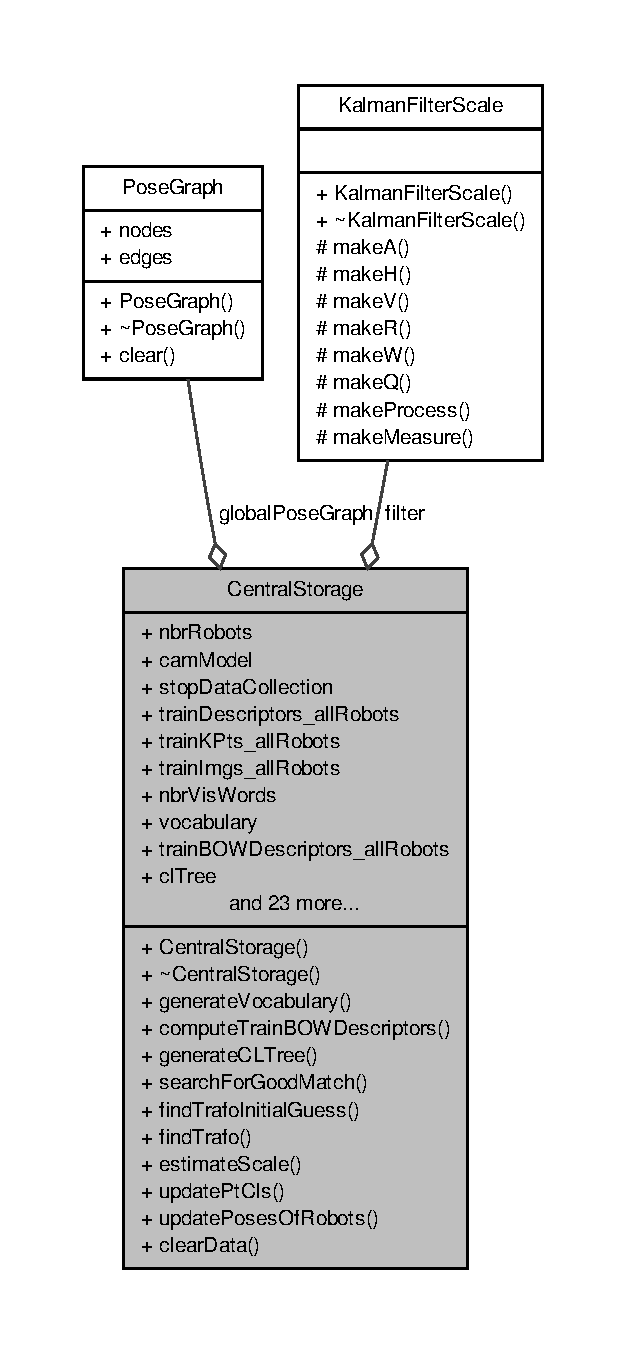
\includegraphics[height=550pt]{classCentralStorage__coll__graph}
\end{center}
\end{figure}
\subsection*{\-Public \-Member \-Functions}
\begin{DoxyCompactItemize}
\item 
\hyperlink{classCentralStorage_a25eac5394f0f460badecfda39c287249}{\-Central\-Storage} (int nbr\-Robots\-Input, int nbr\-Vis\-Words\-Input)
\begin{DoxyCompactList}\small\item\em \-Constructor setting initial values to member variables and initializing detector, extractor, matcher and \-B\-O\-W\-K\-Means\-Trainer. \end{DoxyCompactList}\item 
\hyperlink{classCentralStorage_a02c77a753e14f274385b5df7cfee2f1f}{$\sim$\-Central\-Storage} ()
\item 
void \hyperlink{classCentralStorage_aed7b4357ce0cb743a5c8074b805b51a5}{generate\-Vocabulary} ()
\begin{DoxyCompactList}\small\item\em \-Member function generating vocabulatory (dictionary/ visual words/ ...) and outputting it in \char`\"{}vocab.\-yml\char`\"{}, also saves all descriptors (\-S\-U\-R\-F) of all robots in \char`\"{}train\-Descriptors\-\_\-all\-Robots.\-yml\char`\"{}. \end{DoxyCompactList}\item 
void \hyperlink{classCentralStorage_a925c5d072478a869cc511e11cbe9248d}{compute\-Train\-B\-O\-W\-Descriptors} ()
\item 
void \hyperlink{classCentralStorage_a76ea5d6aa74f139a4db824b679958ce2}{generate\-C\-L\-Tree} ()
\begin{DoxyCompactList}\small\item\em \-Member function generating chow liu tree and outputting it in \char`\"{}cltree.\-yml\char`\"{}. \end{DoxyCompactList}\item 
void \hyperlink{classCentralStorage_a7e6a32a86c37de7871884670cf97d598}{search\-For\-Good\-Match} ()
\item 
void \hyperlink{classCentralStorage_a76c399f09dc7d0083508c1a14f8dd8f3}{find\-Trafo\-Initial\-Guess} ()
\begin{DoxyCompactList}\small\item\em \-Member function calculating an initial guess for the pose of one camera relative to the other camera of two matched images based on matched keypoints \-The result of running, namely p\-Test\-Query (p2nd1st), is stored in storage-\/$>$i\-G\-Map\mbox{[}query\-Img\-Ctr\mbox{]}. \end{DoxyCompactList}\item 
void \hyperlink{classCentralStorage_aac60399a1652a2e63e3efd01d4758a1e}{find\-Trafo} (\-Eigen\-::\-Matrix4f i\-G, \-Eigen\-::\-Matrix4f \&final\-Trafo)
\begin{DoxyCompactList}\small\item\em \-Member function calculating an the pose of one camera relative to the other camera of two matched images based icp with the initial \-Guess calculated in find\-Trafo\-Initial\-Guess \-The result of running, namely p\-Test\-Query (p2nd1st), is stored in ???? \end{DoxyCompactList}\item 
void \hyperlink{classCentralStorage_a250829100ab52dc84a71997246870a69}{estimate\-Scale} ()
\item 
void \hyperlink{classCentralStorage_ac065c164a68a24bb1d5e0ff0b9a41f84}{update\-Pt\-Cls} ()
\item 
void \hyperlink{classCentralStorage_ad0e2f8a4581fe0e61a49b07141442dd2}{update\-Poses\-Of\-Robots} ()
\item 
void \hyperlink{classCentralStorage_a90df91c64ab74dfa7d557f08a27a9cdf}{clear\-Data} ()
\end{DoxyCompactItemize}
\subsection*{\-Public \-Attributes}
\begin{DoxyCompactItemize}
\item 
int \hyperlink{classCentralStorage_a83a67f52de30d339d872138243d42764}{nbr\-Robots}
\item 
image\-\_\-geometry\-::\-Pinhole\-Camera\-Model \hyperlink{classCentralStorage_adfcd7e35336daa5d959f783c9180460f}{cam\-Model}
\item 
bool \hyperlink{classCentralStorage_ac721895aafa60a4fb37c9659aabaed7a}{stop\-Data\-Collection}
\item 
cv\-::\-Mat \hyperlink{classCentralStorage_ad574732df5058d95d650c1187a9ba4f6}{train\-Descriptors\-\_\-all\-Robots}
\item 
vector$<$ vector$<$ \-Key\-Point $>$ $>$ \hyperlink{classCentralStorage_a6eba28072f558f36c2b3a08170f9db74}{train\-K\-Pts\-\_\-all\-Robots}
\item 
vector$<$ cv\-::\-Mat $>$ \hyperlink{classCentralStorage_a673208fa43bab02c4e53077ae45a38e7}{train\-Imgs\-\_\-all\-Robots}
\item 
int \hyperlink{classCentralStorage_a6830253bfbd8a4c03cc317820358d25a}{nbr\-Vis\-Words}
\item 
cv\-::\-Mat \hyperlink{classCentralStorage_a50f04d43d8c1f26725bb2e2e560a494c}{vocabulary}
\item 
cv\-::\-Mat \hyperlink{classCentralStorage_ad22679ec76d8fc9c99226a1bfdd4c410}{train\-B\-O\-W\-Descriptors\-\_\-all\-Robots}
\item 
cv\-::\-Mat \hyperlink{classCentralStorage_a5d9e98c4102f50187f6a034a99ef9793}{cl\-Tree}
\item 
\-B\-O\-W\-K\-Means\-Trainer $\ast$ \hyperlink{classCentralStorage_aa30a8d753544480abd495023cbf62a2f}{\-B\-O\-W\-Trainer}
\item 
\-Ptr$<$ \-Feature\-Detector $>$ \hyperlink{classCentralStorage_a3853e38f8eadbe09da6a1855b29704f7}{detector}
\item 
\-Ptr$<$ \-Descriptor\-Extractor $>$ \hyperlink{classCentralStorage_a8c18048b9cf9171a16d6d9e2fa8f8754}{extractor}
\item 
\-Ptr$<$ \-Descriptor\-Matcher $>$ \hyperlink{classCentralStorage_a8ff5fb67a41c196b5677015e09ff33be}{matcher}
\item 
\-B\-O\-W\-Img\-Descriptor\-Extractor $\ast$ \hyperlink{classCentralStorage_ab1828f1368902fab93265328a6e53063}{bide}
\item 
\-Ptr$<$ of2\-::\-Fab\-Map $>$ \hyperlink{classCentralStorage_a4172d4d2a8509cb0bfbdb4edc8a3707b}{fabmap}
\item 
std\-::map$<$ int, \hyperlink{structkeyFrame}{key\-Frame} $>$ \hyperlink{classCentralStorage_ab477c78726c58cba1b5b14255700ff64}{k\-Frames}
\item 
std\-::map$<$ int, std\-::pair$<$ int, \*
pcl\-::\-Point\-Cloud$<$ pcl\-::\-Point\-X\-Y\-Z $>$ $>$ $>$ \hyperlink{classCentralStorage_a98df05b89e7956601eeff266fbef0754}{pt\-Cls}
\begin{DoxyCompactList}\small\item\em the key for accessing a pt\-Cls corresponds to the the k\-Frames identity number (\-Img\-Ctr), the std\-::pair contains the associated r\-I\-D and the actual \-Pt\-Cl \end{DoxyCompactList}\item 
std\-::map$<$ int, std\-::pair$<$ int, \*
pcl\-::\-Point\-Cloud$<$ pcl\-::\-Point\-X\-Y\-Z $>$ $>$ $>$ \hyperlink{classCentralStorage_ac162077a92cd58a58d19ae7404719490}{pt\-Cls\-In\-Global\-World\-C\-O\-S}
\item 
std\-::map$<$ int, bool $>$ \hyperlink{classCentralStorage_a6b25259119c01d07da15d4e5c9f806f8}{pt\-Cls\-In\-Global\-World\-C\-O\-S\-Updated}
\item 
std\-::map$<$ int, std\-::pair$<$ int, \*
geometry\-\_\-msgs\-::\-Pose\-Stamped $>$ $>$ \hyperlink{classCentralStorage_a9f86101c4abfa538b14ecafbbffb49e8}{local\-Poses}
\item 
std\-::map$<$ int, std\-::pair$<$ int, \*
float $>$ $>$ \hyperlink{classCentralStorage_a77f707a32dbf4d3b76668d2bdb2db060}{local\-Scales}
\begin{DoxyCompactList}\small\item\em \-Saves the scales for all robots and all images. \-I\-M\-P\-O\-R\-T\-A\-N\-T \-N\-O\-T\-E\-: only the latest scale is needed for each robot!!!! (current storage-\/$>$test\-Img\-Ctr!!!) $<$-\/-\/ \-Maybe not true (see \-L\-S\-D \-S\-L\-A\-M 3.\-5 scale for each keyframe) \end{DoxyCompactList}\item 
\hyperlink{classKalmanFilterScale}{\-Kalman\-Filter\-Scale} \hyperlink{classCentralStorage_af952071a5b552f94e01d8667227bfa57}{filter}
\item 
std\-::map$<$ int, float $>$ \hyperlink{classCentralStorage_a017fa3b55ed277d63df2a0937be0ead7}{robot\-Scales}
\item 
std\-::map$<$ int, \-Eigen\-::\-Matrix4f $>$ \hyperlink{classCentralStorage_ae701316885fe7f1366f17ec44393b84b}{p\-Robots\-World}
\item 
std\-::map$<$ int, \hyperlink{classPoseGraph}{\-Pose\-Graph} $>$ \hyperlink{classCentralStorage_a872f54468c1ac5aa5438d3c820cfc5bd}{local\-Pose\-Graphs}
\begin{DoxyCompactList}\small\item\em the key for accessing the local\-Pose\-Graph corresponding to a robot is the corresponding robot \-I\-D r\-I\-D \end{DoxyCompactList}\item 
\hyperlink{classPoseGraph}{\-Pose\-Graph} \hyperlink{classCentralStorage_a710a94a5fbcb985594717f0864405872}{global\-Pose\-Graph}
\begin{DoxyCompactList}\small\item\em all local \-Pose\-Graphs added together \end{DoxyCompactList}\item 
cv\-::\-Mat \hyperlink{classCentralStorage_ab3aae9d93bbccd2a646330cb8812824f}{test\-B\-O\-W\-Descriptors\-\_\-all\-Robots}
\item 
int \hyperlink{classCentralStorage_ac6ecd35e9f6a9d0145f87fb98c6fb923}{test\-Img\-Ctr}
\item 
vector$<$ of2\-::\-I\-Match $>$ \hyperlink{classCentralStorage_af2ce7451320774bb90db744fa46493bd}{matches}
\item 
bool \hyperlink{classCentralStorage_a311e52441ce3ca79a2eac623c58221cc}{bool\-Match}
\item 
std\-::pair$<$ int, int $>$ \hyperlink{classCentralStorage_a393e5d052d921122176d0ebf0a6cfadb}{matched\-Key\-Frames}
\item 
std\-::map$<$ int, std\-::pair$<$ int, \*
int $>$ $>$ \hyperlink{classCentralStorage_a8382babfd80ae718d4f15ddfa5ef5017}{matched\-Key\-Frames\-Map}
\begin{DoxyCompactList}\small\item\em key is the nbr of the query\-Img (\-Img\-Ctr) -\/-\/$>$ access k\-Frame\-: storage-\/$>$k\-Frames\mbox{[} matched\-Key\-Frames\-Map\mbox{[}nbr\mbox{]}.first \mbox{]}, storage-\/$>$k\-Frames\mbox{[} matched\-Key\-Frames\-Map\mbox{[}nbr\mbox{]}.second \mbox{]} \end{DoxyCompactList}\item 
std\-::map$<$ int, std\-::pair\*
$<$ \-Eigen\-::\-Matrix4f, int $>$ $>$ \hyperlink{classCentralStorage_a3ae59bfa3849b3dd984c636e0a9af23a}{i\-G\-Map}
\end{DoxyCompactItemize}


\subsection{\-Detailed \-Description}
\-Class storing all images of all robots, global maps (pose graph and point cloud) 

\-Definition at line 78 of file \-Central\-Storage.\-h.



\subsection{\-Constructor \& \-Destructor \-Documentation}
\hypertarget{classCentralStorage_a25eac5394f0f460badecfda39c287249}{\index{\-Central\-Storage@{\-Central\-Storage}!\-Central\-Storage@{\-Central\-Storage}}
\index{\-Central\-Storage@{\-Central\-Storage}!CentralStorage@{\-Central\-Storage}}
\subsubsection[{\-Central\-Storage}]{\setlength{\rightskip}{0pt plus 5cm}const char {\bf \-Central\-Storage\-::\-Central\-Storage} (
\begin{DoxyParamCaption}
\item[{int}]{nbr\-Robots\-Input, }
\item[{int}]{nbr\-Vis\-Words\-Input}
\end{DoxyParamCaption}
)}}\label{classCentralStorage_a25eac5394f0f460badecfda39c287249}


\-Constructor setting initial values to member variables and initializing detector, extractor, matcher and \-B\-O\-W\-K\-Means\-Trainer. 



\-Definition at line 8 of file \-Central\-Storage.\-cpp.


\begin{DoxyCode}
                                                                       :
                nbrRobots(nbrRobotsInput),
                nbrVisWords(nbrVisWordsInput),
                testImgCtr(0),
                stopDataCollection(false)
                {
//      // Init camera Matrix and distortion coefficients
//      //float camMatArr[3][3] = {{442.777026, 0, 291.591624},{0, 444.581889,
       207.395871},{0, 0, 1}};
//      //float distCoeffsArr[5] = {-0.343887, 0.100088, -0.001316, -0.000163,
       0};
//      //camMat = Mat(3,3,CV_32FC1,camMatArr);
//      //distCoeffs = Mat(5,1,CV_32FC1,distCoeffsArr);



        // Detector, Extractor, Matcher, BOW Img Descriptor, BOW KMeans trainer
    //detector = new
       DynamicAdaptedFeatureDetector(AdjusterAdapter::create("SURF"),150,250,4); //
        //detector = new
       DynamicAdaptedFeatureDetector(AdjusterAdapter::create("SIFT"),400,500,5); //
        //detector = new SiftFeatureDetector(0, 1, 1, 5, 0.9); // nfeatures,
       noctavelayers,contrastthreshold (higher->less features), edgethreshold
       (higher->more features) ,sigma
        detector = new SiftFeatureDetector(0, 4, 0.04, 10, 1.0); // nfeatures,
       noctavelayers,contrastthreshold (higher->less features), edgethreshold
       (higher->more features) ,sigma

//detector = new SiftFeatureDetector(0, 3, 0.15, 5, 0.9);0, 3, 0.15, 5, 0.9

        //extractor = new SurfDescriptorExtractor(500,4,2,false,true);
       //hessian threshold, noctave,noctavelayers,extended,upright
        extractor = new SiftDescriptorExtractor(); //hessian threshold,
       noctave,noctavelayers,extended,upright
        matcher = DescriptorMatcher::create("FlannBased");
        bide =  new BOWImgDescriptorExtractor(extractor, matcher);
        // clustering (nbr clusters = nbr vis words)
        //define Term Criteria
        TermCriteria tc(CV_TERMCRIT_ITER,100,0.001);
        //retries number
        int retries=1;
        //necessary flags
        int flags=KMEANS_PP_CENTERS;
        BOWTrainer = new BOWKMeansTrainer(nbrVisWords,tc,retries,flags);

        // Initializing Kalman Filter for scale estimation
        KalmanFilterScale::Vector x(1);
        x(1) = 1.0;
        static const float _P0[] = {10.0};
        KalmanFilterScale::Matrix P0(1,1,_P0);
        filter.init(x,P0);

        // Initialize global Transforms with identity transform and initialize
       ptClsUpdated to true
        for(int i=1; i<=nbrRobots; ++i) {
                pRobotsWorld[i] = Eigen::Matrix4f::Identity(4,4);
                ptClsInGlobalWorldCOSUpdated[i] = false;
                robotScales[i] = 1.0;
        }

}
\end{DoxyCode}
\hypertarget{classCentralStorage_a02c77a753e14f274385b5df7cfee2f1f}{\index{\-Central\-Storage@{\-Central\-Storage}!$\sim$\-Central\-Storage@{$\sim$\-Central\-Storage}}
\index{$\sim$\-Central\-Storage@{$\sim$\-Central\-Storage}!CentralStorage@{\-Central\-Storage}}
\subsubsection[{$\sim$\-Central\-Storage}]{\setlength{\rightskip}{0pt plus 5cm}{\bf \-Central\-Storage\-::$\sim$\-Central\-Storage} (
\begin{DoxyParamCaption}
{}
\end{DoxyParamCaption}
)}}\label{classCentralStorage_a02c77a753e14f274385b5df7cfee2f1f}


\-Definition at line 59 of file \-Central\-Storage.\-cpp.


\begin{DoxyCode}
{}
\end{DoxyCode}


\subsection{\-Member \-Function \-Documentation}
\hypertarget{classCentralStorage_a90df91c64ab74dfa7d557f08a27a9cdf}{\index{\-Central\-Storage@{\-Central\-Storage}!clear\-Data@{clear\-Data}}
\index{clear\-Data@{clear\-Data}!CentralStorage@{\-Central\-Storage}}
\subsubsection[{clear\-Data}]{\setlength{\rightskip}{0pt plus 5cm}void {\bf \-Central\-Storage\-::clear\-Data} (
\begin{DoxyParamCaption}
{}
\end{DoxyParamCaption}
)}}\label{classCentralStorage_a90df91c64ab74dfa7d557f08a27a9cdf}


\-Definition at line 479 of file \-Central\-Storage.\-cpp.


\begin{DoxyCode}
                               {
        this->kFrames.clear();

        this->ptCls.clear();
        this->ptClsInGlobalWorldCOS.clear();
        this->ptClsInGlobalWorldCOSUpdated.clear();

        this->localPoses.clear();
        this->localScales.clear();
        this->robotScales.clear();

        this->pRobotsWorld.clear();
        this->localPoseGraphs.clear();

        globalPoseGraph.clear();

        this->testBOWDescriptors_allRobots.release();
        this->testImgCtr = 0;

        this->matches.clear();
        this->boolMatch = false;
        this->matchedKeyFrames = std::make_pair(-1,-1);
        this->matchedKeyFramesMap.clear();

        this->iGMap.clear();
}
\end{DoxyCode}
\hypertarget{classCentralStorage_a925c5d072478a869cc511e11cbe9248d}{\index{\-Central\-Storage@{\-Central\-Storage}!compute\-Train\-B\-O\-W\-Descriptors@{compute\-Train\-B\-O\-W\-Descriptors}}
\index{compute\-Train\-B\-O\-W\-Descriptors@{compute\-Train\-B\-O\-W\-Descriptors}!CentralStorage@{\-Central\-Storage}}
\subsubsection[{compute\-Train\-B\-O\-W\-Descriptors}]{\setlength{\rightskip}{0pt plus 5cm}void {\bf \-Central\-Storage\-::compute\-Train\-B\-O\-W\-Descriptors} (
\begin{DoxyParamCaption}
{}
\end{DoxyParamCaption}
)}}\label{classCentralStorage_a925c5d072478a869cc511e11cbe9248d}


\-Definition at line 67 of file \-Central\-Storage.\-cpp.


\begin{DoxyCode}
                                                {
        int imgCtr = 0;
        cv::Mat BOWDescriptors;

        std::vector<cv::Mat>::iterator itImg;
        for(itImg = this->trainImgs_allRobots.begin(); itImg != this->
      trainImgs_allRobots.end(); ++itImg) {
                this->bide->compute(*itImg, this->trainKPts_allRobots[imgCtr], 
      BOWDescriptors);
                this->trainBOWDescriptors_allRobots.push_back(BOWDescriptors);
                imgCtr = imgCtr + 1;
        }
}
\end{DoxyCode}
\hypertarget{classCentralStorage_a250829100ab52dc84a71997246870a69}{\index{\-Central\-Storage@{\-Central\-Storage}!estimate\-Scale@{estimate\-Scale}}
\index{estimate\-Scale@{estimate\-Scale}!CentralStorage@{\-Central\-Storage}}
\subsubsection[{estimate\-Scale}]{\setlength{\rightskip}{0pt plus 5cm}void {\bf \-Central\-Storage\-::estimate\-Scale} (
\begin{DoxyParamCaption}
{}
\end{DoxyParamCaption}
)}}\label{classCentralStorage_a250829100ab52dc84a71997246870a69}


\-Definition at line 265 of file \-Central\-Storage.\-cpp.


\begin{DoxyCode}
                                   {
        cout << "       estimate scale " << endl;

        // if query = robot 2
        // iGTrafo = pC1C2 = tC2C1
        int queryImgNbr = this->testImgCtr;
        int testImgNbr = matchedKeyFramesMap[queryImgNbr].second;
        Eigen::Matrix4f iGTrafo = this->iGMap[queryImgNbr].first;
        keyFrame queryKF, testKF;


        queryKF = this->kFrames[queryImgNbr];
        testKF = this->kFrames[testImgNbr];
        int queryRID = queryKF.rID;
        int testRID = testKF.rID;

        // Extract descriptors from imgs
        Mat queryImgDescr, testImgDescr;
        this->extractor->compute( queryKF.img, queryKF.KPts, queryImgDescr );
        this->extractor->compute( testKF.img, testKF.KPts, testImgDescr );

        // match descriptors
        std::vector< DMatch > resultingMatches;
        this->matcher->match(queryImgDescr,testImgDescr,resultingMatches);

        vector<Point2f> matched2DPtsQuery, matched2DPtsTest;
        vector<Eigen::Vector3f> matched3DPtsQuery, matched3DPtsTest;
        //vector<float> measurements;
        Eigen::Vector3f matched3DPtQuery(0.0,0.0,0.0), matched3DPtTest(0.0,0.0,
      0.0);

        vector<KeyPoint> matchedQueryKPts, matchedTestKPts;
        for (int i = 0; i < resultingMatches.size(); ++i)       {
                matchedQueryKPts.push_back(queryKF.KPts[resultingMatches[i].
      queryIdx]);
                matchedTestKPts.push_back(testKF.KPts[resultingMatches[i].
      trainIdx]);
        }
//      HelperFcts::displayImageKPts("queryImg", queryKF.img,
       matchedQueryKPts);
//      HelperFcts::displayImageKPts("testImg", testKF.img, matchedTestKPts);
//      HelperFcts::displayMatches("matches", queryKF.img, testKF.img,
       queryKF.KPts, testKF.KPts, resultingMatches);
//      waitKey(10000);

        for (int i = 0; i < resultingMatches.size(); ++i)       {
                Point2f matched2DPtQuery = queryKF.KPts[resultingMatches[i].
      queryIdx].pt;
                Point2f matched2DPtTest = testKF.KPts[resultingMatches[i].
      trainIdx].pt;

                HelperFcts::calc3DPt(matched2DPtQuery, queryKF.fx, queryKF.fy, 
      queryKF.cx, queryKF.cy, queryKF.idepth, matched3DPtQuery);
                //HelperFcts::transform3DPt(queryKF.camToRobot,
       matched3DPtQuery, matched3DPtQuery);


                HelperFcts::calc3DPt(matched2DPtTest, testKF.fx, testKF.fy, 
      testKF.cx, testKF.cy, testKF.idepth, matched3DPtTest);
                // iGTrafo = pC1C2 = tC2C1
                // iGTrafo = pC2C1 = tC1C2
                Eigen::Matrix4f iGTrafoInv(Eigen::Matrix4f::Identity(4,4));
                HelperFcts::invTrafo(iGTrafo, iGTrafoInv);
                HelperFcts::transform3DPt(iGTrafoInv, matched3DPtQuery, 
      matched3DPtQuery);


                KalmanFilterScale::Vector u(0);
                KalmanFilterScale::Vector z(3);
                for(int i=0 ; i<3 ; ++i) {

                        float measurement = matched3DPtTest(i)/matched3DPtQuery
      (i);
                        z(i+1) = measurement;
                }
                this->filter.step(u,z);
        }
        cout << "scale estimate:        " << this->filter.getX()(1) << endl << 
      "cov:    " << this->filter.calculateP()(1,1) << endl;
        this->robotScales[queryRID] = this->filter.getX()(1);
}
\end{DoxyCode}
\hypertarget{classCentralStorage_aac60399a1652a2e63e3efd01d4758a1e}{\index{\-Central\-Storage@{\-Central\-Storage}!find\-Trafo@{find\-Trafo}}
\index{find\-Trafo@{find\-Trafo}!CentralStorage@{\-Central\-Storage}}
\subsubsection[{find\-Trafo}]{\setlength{\rightskip}{0pt plus 5cm}const char {\bf \-Central\-Storage\-::find\-Trafo} (
\begin{DoxyParamCaption}
\item[{\-Eigen\-::\-Matrix4f}]{i\-G, }
\item[{\-Eigen\-::\-Matrix4f \&}]{final\-Trafo}
\end{DoxyParamCaption}
)}}\label{classCentralStorage_aac60399a1652a2e63e3efd01d4758a1e}


\-Member function calculating an the pose of one camera relative to the other camera of two matched images based icp with the initial \-Guess calculated in find\-Trafo\-Initial\-Guess \-The result of running, namely p\-Test\-Query (p2nd1st), is stored in ???? 



\-Definition at line 245 of file \-Central\-Storage.\-cpp.


\begin{DoxyCode}
                                                                           {

        int queryImgCtrMatch = this->testImgCtr;
        int testImgCtrMatch = this->matchedKeyFramesMap[queryImgCtrMatch].
      second;

        pcl::PointCloud<pcl::PointXYZ>::Ptr ptClToPtrSource(new 
      pcl::PointCloud<pcl::PointXYZ>());
        pcl::PointCloud<pcl::PointXYZ>::Ptr ptClToPtrTarget(new 
      pcl::PointCloud<pcl::PointXYZ>());
        *ptClToPtrSource = this->ptCls[queryImgCtrMatch].second;
        *ptClToPtrTarget = this->ptCls[testImgCtrMatch].second;

         pcl::IterativeClosestPoint<pcl::PointXYZ, pcl::PointXYZ> icp;
         icp.setInputSource(ptClToPtrSource);
         icp.setInputTarget(ptClToPtrTarget);

         pcl::PointCloud<pcl::PointXYZ> Final;
         icp.align(Final, iG);

         finalTrafo = icp.getFinalTransformation();
}
\end{DoxyCode}
\hypertarget{classCentralStorage_a76c399f09dc7d0083508c1a14f8dd8f3}{\index{\-Central\-Storage@{\-Central\-Storage}!find\-Trafo\-Initial\-Guess@{find\-Trafo\-Initial\-Guess}}
\index{find\-Trafo\-Initial\-Guess@{find\-Trafo\-Initial\-Guess}!CentralStorage@{\-Central\-Storage}}
\subsubsection[{find\-Trafo\-Initial\-Guess}]{\setlength{\rightskip}{0pt plus 5cm}const char {\bf \-Central\-Storage\-::find\-Trafo\-Initial\-Guess} (
\begin{DoxyParamCaption}
{}
\end{DoxyParamCaption}
)}}\label{classCentralStorage_a76c399f09dc7d0083508c1a14f8dd8f3}


\-Member function calculating an initial guess for the pose of one camera relative to the other camera of two matched images based on matched keypoints \-The result of running, namely p\-Test\-Query (p2nd1st), is stored in storage-\/$>$i\-G\-Map\mbox{[}query\-Img\-Ctr\mbox{]}. 



\-Definition at line 156 of file \-Central\-Storage.\-cpp.


\begin{DoxyCode}
                                           {

        cout << "               find IG" << endl;
        int queryImgNbr = this->testImgCtr;
        int testImgNbr = matchedKeyFramesMap[queryImgNbr].second;

        keyFrame queryKF, testKF;

        queryKF = this->kFrames[queryImgNbr];
        testKF = this->kFrames[testImgNbr];
        int queryRID = queryKF.rID;
        int testRID = testKF.rID;
        // Extract descriptors from imgs
        Mat queryImgDescr, testImgDescr;
        this->extractor->compute(queryKF.img,queryKF.KPts,queryImgDescr);
        this->extractor->compute(testKF.img,testKF.KPts,testImgDescr);

        // match descriptors
        std::vector< DMatch > resultingMatches;
        this->matcher->match(queryImgDescr,testImgDescr,resultingMatches);

        // Filter out bad matches
        double max_dist = 0; double min_dist = 100;
        //-- Quick calculation of max and min distances between keypoints
        for( int i = 0; i < queryImgDescr.rows; i++ ) {
                double dist = resultingMatches[i].distance;
                if( dist < min_dist ) min_dist = dist;
                if( dist > max_dist ) max_dist = dist;
        }
        std::vector< DMatch > good_matches;
        for( int i = 0; i < queryImgDescr.rows; i++ ) {
                if( resultingMatches[i].distance <= max(3*min_dist, 10.0) ) {
                        good_matches.push_back( resultingMatches[i]);
                }
        }


        HelperFcts::displayMatches("testmatches",queryKF.img,testKF.img,queryKF
      .KPts,testKF.KPts,good_matches, true);

        //derive correspondences based on random point-cloud
        bearingVector_t bearingVectorQuery,bearingVectorTest;
        bearingVectors_t bearingVectorsQuery;
        bearingVectors_t bearingVectorsTest;

        vector<Point2f> matchedPtsQuery, matchedPtsTest;
        for (int i = 0; i < good_matches.size(); ++i)
        {
                Point2f matchedPtQuery = queryKF.KPts[good_matches[i].queryIdx]
      .pt;
                Point2f matchedPtTest = testKF.KPts[good_matches[i].trainIdx].
      pt;

                matchedPtsQuery.push_back(matchedPtQuery);
                matchedPtsTest.push_back(matchedPtTest);

                bearingVectorQuery[0] = matchedPtQuery.x/sqrt(matchedPtQuery.x*
      matchedPtQuery.x + matchedPtQuery.y*matchedPtQuery.y + 1.0);
                bearingVectorQuery[1] = matchedPtQuery.y/sqrt(matchedPtQuery.x*
      matchedPtQuery.x + matchedPtQuery.y*matchedPtQuery.y + 1.0);
                bearingVectorQuery[2] = 1.0;//sqrt(1.0 -
       matchedPtQuery.x*matchedPtQuery.x - matchedPtQuery.y*matchedPtQuery.y);
                bearingVectorQuery.normalize();

                bearingVectorTest[0] = matchedPtTest.x/sqrt(matchedPtTest.x*
      matchedPtTest.x + matchedPtTest.y*matchedPtTest.y + 1.0);
                bearingVectorTest[1] = matchedPtTest.y/sqrt(matchedPtTest.x*
      matchedPtTest.x + matchedPtTest.y*matchedPtTest.y + 1.0);
                //sqrt(1.0 - matchedPtTest.x*matchedPtTest.x -
       matchedPtTest.y*matchedPtTest.y)
                bearingVectorTest[2] = 1.0;//sqrt(1.0 -
       matchedPtTest.x*matchedPtTest.x - matchedPtTest.y*matchedPtTest.y);
                bearingVectorTest.normalize();

                bearingVectorsQuery.push_back(bearingVectorQuery);
                bearingVectorsTest.push_back(bearingVectorTest);

        }

        relative_pose::CentralRelativeAdapter adapter(bearingVectorsQuery,
      bearingVectorsTest);
        sac::Ransac<sac_problems::relative_pose::CentralRelativePoseSacProblem>
       ransac;
        
      boost::shared_ptr<sac_problems::relative_pose::CentralRelativePoseSacProblem> relposeproblem_ptr(new 
      sac_problems::relative_pose::CentralRelativePoseSacProblem(adapter,
      sac_problems::relative_pose::CentralRelativePoseSacProblem::NISTER));
        ransac.sac_model_ = relposeproblem_ptr;
        ransac.threshold_ = 2.0*(1.0 - cos(atan(sqrt(2.0)*0.5/800.0)));
        ransac.max_iterations_ = 50;

        ransac.computeModel();
        transformation_t pCamTestCamQueryOpenGV = ransac.model_coefficients_;


        Eigen::Matrix4f iG(Eigen::Matrix4f::Identity(4,4));
        Eigen::Matrix4d iGdouble(Eigen::Matrix4d::Identity(4,4));
        iGdouble.block(0,0,3,4) = pCamTestCamQueryOpenGV;
        iG = iGdouble.cast<float>();

        this->iGMap[queryImgNbr] = std::make_pair(iG,testImgNbr);

}
\end{DoxyCode}
\hypertarget{classCentralStorage_a76ea5d6aa74f139a4db824b679958ce2}{\index{\-Central\-Storage@{\-Central\-Storage}!generate\-C\-L\-Tree@{generate\-C\-L\-Tree}}
\index{generate\-C\-L\-Tree@{generate\-C\-L\-Tree}!CentralStorage@{\-Central\-Storage}}
\subsubsection[{generate\-C\-L\-Tree}]{\setlength{\rightskip}{0pt plus 5cm}const char {\bf \-Central\-Storage\-::generate\-C\-L\-Tree} (
\begin{DoxyParamCaption}
{}
\end{DoxyParamCaption}
)}}\label{classCentralStorage_a76ea5d6aa74f139a4db824b679958ce2}


\-Member function generating chow liu tree and outputting it in \char`\"{}cltree.\-yml\char`\"{}. 



\-Definition at line 79 of file \-Central\-Storage.\-cpp.


\begin{DoxyCode}
                                    {
        of2::ChowLiuTree treeBuilder;
        treeBuilder.add(this->trainBOWDescriptors_allRobots);
        this->clTree = treeBuilder.make();
}
\end{DoxyCode}
\hypertarget{classCentralStorage_aed7b4357ce0cb743a5c8074b805b51a5}{\index{\-Central\-Storage@{\-Central\-Storage}!generate\-Vocabulary@{generate\-Vocabulary}}
\index{generate\-Vocabulary@{generate\-Vocabulary}!CentralStorage@{\-Central\-Storage}}
\subsubsection[{generate\-Vocabulary}]{\setlength{\rightskip}{0pt plus 5cm}const char {\bf \-Central\-Storage\-::generate\-Vocabulary} (
\begin{DoxyParamCaption}
{}
\end{DoxyParamCaption}
)}}\label{classCentralStorage_aed7b4357ce0cb743a5c8074b805b51a5}


\-Member function generating vocabulatory (dictionary/ visual words/ ...) and outputting it in \char`\"{}vocab.\-yml\char`\"{}, also saves all descriptors (\-S\-U\-R\-F) of all robots in \char`\"{}train\-Descriptors\-\_\-all\-Robots.\-yml\char`\"{}. 



\-Definition at line 62 of file \-Central\-Storage.\-cpp.


\begin{DoxyCode}
                                        {
        this->BOWTrainer->add(this->trainDescriptors_allRobots);
        this->vocabulary = this->BOWTrainer->cluster(); // Returns the cluster
       centers (descriptors are clustered into nbr vis words)
}
\end{DoxyCode}
\hypertarget{classCentralStorage_a7e6a32a86c37de7871884670cf97d598}{\index{\-Central\-Storage@{\-Central\-Storage}!search\-For\-Good\-Match@{search\-For\-Good\-Match}}
\index{search\-For\-Good\-Match@{search\-For\-Good\-Match}!CentralStorage@{\-Central\-Storage}}
\subsubsection[{search\-For\-Good\-Match}]{\setlength{\rightskip}{0pt plus 5cm}void {\bf \-Central\-Storage\-::search\-For\-Good\-Match} (
\begin{DoxyParamCaption}
{}
\end{DoxyParamCaption}
)}}\label{classCentralStorage_a7e6a32a86c37de7871884670cf97d598}


\-Definition at line 85 of file \-Central\-Storage.\-cpp.


\begin{DoxyCode}
                                        {
        //FOR TMR
        // dont consider first several imsg
        // add consecutive if from other robot
        // no match if other robot has some there
        if(this->testImgCtr>0) {

                ostringstream convStringFileName, convStringContent;
                string matchedImgsFileName, matchedImgsContent;
                int kFrameNbr = -10000;
                int rID = this->kFrames[this->testImgCtr].rID;
                vector<of2::IMatch>::const_iterator it;
                float maxLikeli = 0;
                float matchCurrent(0.0), matchLast(0.0), matchSecondLast(0.0);
                //int nbrImgs = (int) -0.5+(1/4+2*this->matches.size())^(1/2);
                // for last query Img (last keyframe) loop through all
       (test)imgs except the query img on its own (query img - query img :
       this->matches.end()-this->testImgCtr-1)
                for(it = this->matches.end()-this->testImgCtr; it != this->
      matches.end(); ++it) {

//                      if(this->testImgCtr < 30) { // dont consider matches
       among the first 6 keyframes
//                      if(this->testImgCtr < 8) { // dont consider matches
       among the first 6 keyframes
                        if(this->testImgCtr < 45) { // dont consider matches
       among the first 6 keyframes
                                continue;
                        }


//                      if(it->match < 0.75) {
                        if(it->match < 0.75) {
//                              cout << "               match probability too
       low" << endl;
                                continue;
                        }

                        if(it->imgIdx != -1) { // comparing query Img to
       testing Img associated with kFrameNbr
                                kFrameNbr = it->imgIdx;
                        }
                        else if(it->imgIdx == -1) { // comparing query Img to
       itself
//                              cout << "               compared to its own2"
       << endl;
                                kFrameNbr = this->kFrames.size()-1;
                                continue; // Do not test to itself
                        }

                        if(this->kFrames[this->testImgCtr].rID == this->kFrames
      [kFrameNbr].rID) { // No matches of same robot
//                              cout << "               same robot ID" << endl;
                                continue;
                        }

                        // name of file determines queryImg specifications
                        convStringFileName << "matchingImgs/robot" << this->
      kFrames[this->testImgCtr].rID << "MatchedImgsQueryImg" << this->kFrames[this->
      testImgCtr].fID << ".yml";
                        matchedImgsFileName = convStringFileName.str();

                        convStringContent << "robot: " << this->kFrames[
      kFrameNbr].rID << "   MatchedImg: " << this->kFrames[kFrameNbr].fID << "   MatchProbab:
       " << it->match << "     ";
                        matchedImgsContent = convStringContent.str();

                        this->matchedKeyFrames.first = this->testImgCtr; //
       query Img
                        this->matchedKeyFrames.second = kFrameNbr; // matched
       test Img
                        this->matchedKeyFramesMap.insert(std::pair<int,
      std::pair <int,int> >(this->testImgCtr,this->matchedKeyFrames)); // store with key "nbr
       of query image (= this->testImgCtr)"
                        if(!matchedImgsContent.empty()) {
                                cout << "               GOOD MATCH" << endl;
                                HelperFcts::saveStringToFile(matchedImgsContent
      , matchedImgsFileName);
                                this->boolMatch = true;

                                // set bool to update map
                                typedef std::map<int,bool> ptClUpdatedMap;
                                for (ptClUpdatedMap::iterator it = this->
      ptClsInGlobalWorldCOSUpdated.begin(); it!=this->ptClsInGlobalWorldCOSUpdated.
      end(); ++it) {
                                        it->second = false;
                                }
                        }
                } // END for loop through matches

        } // END if this->testImgCtr > 0
}
\end{DoxyCode}
\hypertarget{classCentralStorage_ad0e2f8a4581fe0e61a49b07141442dd2}{\index{\-Central\-Storage@{\-Central\-Storage}!update\-Poses\-Of\-Robots@{update\-Poses\-Of\-Robots}}
\index{update\-Poses\-Of\-Robots@{update\-Poses\-Of\-Robots}!CentralStorage@{\-Central\-Storage}}
\subsubsection[{update\-Poses\-Of\-Robots}]{\setlength{\rightskip}{0pt plus 5cm}void {\bf \-Central\-Storage\-::update\-Poses\-Of\-Robots} (
\begin{DoxyParamCaption}
{}
\end{DoxyParamCaption}
)}}\label{classCentralStorage_ad0e2f8a4581fe0e61a49b07141442dd2}


\-Definition at line 334 of file \-Central\-Storage.\-cpp.


\begin{DoxyCode}
                                         {
        cout << "       Update Poses of Robots" << endl;

        // check if any ptcl has update neccessary
        typedef std::map<int,bool> ptClUpdatedMap;
        vector<int> rIDToUpdate;
        for (ptClUpdatedMap::iterator it = this->ptClsInGlobalWorldCOSUpdated.
      begin(); it!=this->ptClsInGlobalWorldCOSUpdated.end(); ++it) {
                if(it->second == false) {
                        rIDToUpdate.push_back(it->first);
                }
        }

        if(this->matchedKeyFramesMap.empty()) { // no matches yet
                cout << "               No matches yet" << endl;
                this->pRobotsWorld[1] = Eigen::Matrix4f::Identity(4,4);

                Eigen::Matrix4f initTrafo(Eigen::Matrix4f::Identity(4,4));
                initTrafo.block(0,3,3,1) << 0,0,0;
                this->pRobotsWorld[2] = initTrafo;
        }
        else if( !this->matchedKeyFramesMap.empty() && !rIDToUpdate.empty() ) {
       // there is a new match
                for(int i=1; i<=this->nbrRobots; ++i) { // iterate through all
       robots
                        if(i == 1) { // update global pose of robot 1
                                this->pRobotsWorld[i] = 
      Eigen::Matrix4f::Identity(4,4);
                                this->ptClsInGlobalWorldCOSUpdated[i] = false;
                        }
                        else { // update global pose of robot 2
                                // pRobotsWorld[2] = pRobot2World =
       tWorldRobot2
                                // = tWorldRobot1 * tRobot1Cam1 * tCam1Cam2 *
       tCam2Robot2
                                // = Identity     * pCam1Robot1 * pCam2Cam1 *
       pRobot2Cam2
                                // = Identity     * pCam1Robot1 * pCam2Cam1 *
       pCam2Robot2^(-1)

                                int matchQueryImgCtr = this->matchedKeyFramesMap
      .rbegin()->second.first;
                                int matchTestImgCtr = this->matchedKeyFramesMap
      .rbegin()->second.second;

                                if(this->localPoses[matchQueryImgCtr].first == 
      1) {
                                        // R1 = Query, R2 = Test
                                        Eigen::Matrix4f pCam1Robot1(
      Eigen::Matrix4f::Identity(4,4));
                                        HelperFcts::poseStampedROSToMatrix4f(
      this->localPoses[matchQueryImgCtr].second, pCam1Robot1);

                                        Eigen::Matrix4f pCam2Cam1(
      Eigen::Matrix4f::Identity(4,4));
                                        pCam2Cam1 = this->iGMap[
      matchQueryImgCtr].first;

                                        Eigen::Matrix4f pRobot2Cam2(
      Eigen::Matrix4f::Identity(4,4));
                                        Eigen::Matrix4f pCam2Robot2(
      Eigen::Matrix4f::Identity(4,4));
                                        HelperFcts::poseStampedROSToMatrix4f(
      this->localPoses[matchTestImgCtr].second, pCam2Robot2);
                                        HelperFcts::invTrafo(pCam2Robot2, 
      pRobot2Cam2);
                                        //this->pRobotsWorld[rID] =
       Eigen::Matrix4f::Identity(4,4) * pCam1Robot1 * pCam2Cam1 * pRobot2Cam2;

                                        Eigen::Matrix4f scale(
      Eigen::Matrix4f::Identity(4,4));
                                        scale.block(0,0,3,3) = 1/this->
      robotScales[i]*Eigen::Matrix3f::Identity(3,3);

                                        Eigen::Matrix4f invTmp;
                                        HelperFcts::invTrafo(
      Eigen::Matrix4f::Identity(4,4) * pCam1Robot1 * pRobot2Cam2 * scale, invTmp);

                                        this->pRobotsWorld[i] = 
      Eigen::Matrix4f::Identity(4,4) * pCam1Robot1 * pRobot2Cam2 * scale;
                                        //this->pRobotsWorld[i] =
       Eigen::Matrix4f::Identity(4,4) * pCam1Robot1 * pRobot2Cam2 * 1;
                                        cout << "this->pRobotsWorld[i]: " << 
      this->pRobotsWorld[i] << endl;
                                }
                                else if(this->localPoses[matchQueryImgCtr].
      first == 2) {
                                        // R2 = Query, R1 = Test
                                        Eigen::Matrix4f pCam1Robot1(
      Eigen::Matrix4f::Identity(4,4));
                                        HelperFcts::poseStampedROSToMatrix4f(
      this->localPoses[matchTestImgCtr].second, pCam1Robot1);

                                        Eigen::Matrix4f pCam2Cam1(
      Eigen::Matrix4f::Identity(4,4));
                                        Eigen::Matrix4f pCam1Cam2(
      Eigen::Matrix4f::Identity(4,4));
                                        pCam1Cam2 = this->iGMap[
      matchQueryImgCtr].first;
                                        HelperFcts::invTrafo(pCam1Cam2, 
      pCam2Cam1);

                                        Eigen::Matrix4f pRobot2Cam2(
      Eigen::Matrix4f::Identity(4,4));
                                        Eigen::Matrix4f pCam2Robot2(
      Eigen::Matrix4f::Identity(4,4));
                                        HelperFcts::poseStampedROSToMatrix4f(
      this->localPoses[matchQueryImgCtr].second, pCam2Robot2);
                                        HelperFcts::invTrafo(pCam2Robot2, 
      pRobot2Cam2);
                                        //this->pRobotsWorld[rID] =
       Eigen::Matrix4f::Identity(4,4) * pCam1Robot1 * pCam2Cam1 * pRobot2Cam2;

                                        Eigen::Matrix4f scale(
      Eigen::Matrix4f::Identity(4,4));
                                        scale.block(0,0,3,3) = 1/this->
      robotScales[i]*Eigen::Matrix3f::Identity(3,3);

                                        Eigen::Matrix4f invTmp;
                                        HelperFcts::invTrafo(
      Eigen::Matrix4f::Identity(4,4) * pCam1Robot1 * pRobot2Cam2 * scale, invTmp);

                                        this->pRobotsWorld[i] = 
      Eigen::Matrix4f::Identity(4,4) * pCam1Robot1 * pRobot2Cam2 * scale;
                                        //this->pRobotsWorld[i] =
       Eigen::Matrix4f::Identity(4,4) * pCam1Robot1 * pRobot2Cam2 * 1;
                                        cout << "this->pRobotsWorld[i]: " << 
      this->pRobotsWorld[i] << endl;

                                }
                                this->ptClsInGlobalWorldCOSUpdated[i] = false;
                        }
                }
        }
}
\end{DoxyCode}
\hypertarget{classCentralStorage_ac065c164a68a24bb1d5e0ff0b9a41f84}{\index{\-Central\-Storage@{\-Central\-Storage}!update\-Pt\-Cls@{update\-Pt\-Cls}}
\index{update\-Pt\-Cls@{update\-Pt\-Cls}!CentralStorage@{\-Central\-Storage}}
\subsubsection[{update\-Pt\-Cls}]{\setlength{\rightskip}{0pt plus 5cm}void {\bf \-Central\-Storage\-::update\-Pt\-Cls} (
\begin{DoxyParamCaption}
{}
\end{DoxyParamCaption}
)}}\label{classCentralStorage_ac065c164a68a24bb1d5e0ff0b9a41f84}


\-Definition at line 426 of file \-Central\-Storage.\-cpp.


\begin{DoxyCode}
                                 {
        cout << "       Update PtCls" << endl;

        /* Naming conventions:
         * p: pose
         * t: coordinate transformation
         * pCOS2COS1:  pose of COS2 relative to COS1 (expressed in COS1)
         * tCOS2COS1:  coordinate transformation from COS1 to COS2 (transforms
       representation of 3D coords in COS1 to representation of same 3D points in COS2)
         * Robot: initial Robot coordinate system (initial pose of robot at
       initialization of SLAM robot)
         * Cam: camera coordinate system of corresponding robot (current pose
       of camera and robot - transformation between current robot COS and camera COS is
       assumed to be identity)
         * World: world coordinate system, equivalent to initial robot
       coordinate system of robot with robot ID rID=1
         */
        Eigen::Matrix4f pRobotWorld(Eigen::Matrix4f::Identity(4,4));
        Eigen::Matrix4f pWorldRobot(Eigen::Matrix4f::Identity(4,4));
        Eigen::Matrix4f tWorldRobot(Eigen::Matrix4f::Identity(4,4));

        typedef std::map<int,bool> ptClUpdatedMap;
        typedef std::vector<int> rIDToUpdateVec;
        typedef std::map<int,std::pair <int,pcl::PointCloud<pcl::PointXYZ> > > 
      ptClMap;

        // check robot ID for which ptcls can be updated
        vector<int> rIDToUpdate;
        for (ptClUpdatedMap::iterator it = this->ptClsInGlobalWorldCOSUpdated.
      begin(); it!=this->ptClsInGlobalWorldCOSUpdated.end(); ++it) {
                if(it->second == false) {
                        cout << "               PtCls to update: " << it->first
       << endl;
                        rIDToUpdate.push_back(it->first);
                }
        }

        if(rIDToUpdate.empty()) { // all ptcls up-to-date
                cout << "               All PtCls up-to-date" << endl;
        }
        else { // update ptcls
                // update all ptcls from all robot IDs in rIDToUpdate
                for(rIDToUpdateVec::iterator itVec=rIDToUpdate.begin(); itVec<
      rIDToUpdate.end(); ++itVec) {
                        // iterate through all robots that need their ptCls to
       be updated

                        for (ptClMap::iterator it = this->ptCls.begin(); it!=
      this->ptCls.end(); ++it) {
                                // iterate through all ptcls
                                if( (it->second.first == *itVec) ) {
                                        // check if the corresponding robot
       needs update
                                        this->ptClsInGlobalWorldCOS[it->first].
      first = it->second.first;
                                        pRobotWorld = this->pRobotsWorld[*itVec
      ];
                                        tWorldRobot = pRobotWorld;
                                        HelperFcts::invTrafo(pRobotWorld,
      pWorldRobot);
                                        pcl::transformPointCloud(it->second.
      second, this->ptClsInGlobalWorldCOS[it->first].second, pRobotWorld);
                                }
                        }
                        this->ptClsInGlobalWorldCOSUpdated[*itVec] = true;
                }
        }
}
\end{DoxyCode}


\subsection{\-Member \-Data \-Documentation}
\hypertarget{classCentralStorage_ab1828f1368902fab93265328a6e53063}{\index{\-Central\-Storage@{\-Central\-Storage}!bide@{bide}}
\index{bide@{bide}!CentralStorage@{\-Central\-Storage}}
\subsubsection[{bide}]{\setlength{\rightskip}{0pt plus 5cm}\-B\-O\-W\-Img\-Descriptor\-Extractor$\ast$ {\bf \-Central\-Storage\-::bide}}}\label{classCentralStorage_ab1828f1368902fab93265328a6e53063}


\-Definition at line 103 of file \-Central\-Storage.\-h.

\hypertarget{classCentralStorage_a311e52441ce3ca79a2eac623c58221cc}{\index{\-Central\-Storage@{\-Central\-Storage}!bool\-Match@{bool\-Match}}
\index{bool\-Match@{bool\-Match}!CentralStorage@{\-Central\-Storage}}
\subsubsection[{bool\-Match}]{\setlength{\rightskip}{0pt plus 5cm}bool {\bf \-Central\-Storage\-::bool\-Match}}}\label{classCentralStorage_a311e52441ce3ca79a2eac623c58221cc}


\-Definition at line 142 of file \-Central\-Storage.\-h.

\hypertarget{classCentralStorage_aa30a8d753544480abd495023cbf62a2f}{\index{\-Central\-Storage@{\-Central\-Storage}!\-B\-O\-W\-Trainer@{\-B\-O\-W\-Trainer}}
\index{\-B\-O\-W\-Trainer@{\-B\-O\-W\-Trainer}!CentralStorage@{\-Central\-Storage}}
\subsubsection[{\-B\-O\-W\-Trainer}]{\setlength{\rightskip}{0pt plus 5cm}\-B\-O\-W\-K\-Means\-Trainer$\ast$ {\bf \-Central\-Storage\-::\-B\-O\-W\-Trainer}}}\label{classCentralStorage_aa30a8d753544480abd495023cbf62a2f}


\-Definition at line 99 of file \-Central\-Storage.\-h.

\hypertarget{classCentralStorage_adfcd7e35336daa5d959f783c9180460f}{\index{\-Central\-Storage@{\-Central\-Storage}!cam\-Model@{cam\-Model}}
\index{cam\-Model@{cam\-Model}!CentralStorage@{\-Central\-Storage}}
\subsubsection[{cam\-Model}]{\setlength{\rightskip}{0pt plus 5cm}image\-\_\-geometry\-::\-Pinhole\-Camera\-Model {\bf \-Central\-Storage\-::cam\-Model}}}\label{classCentralStorage_adfcd7e35336daa5d959f783c9180460f}


\-Definition at line 83 of file \-Central\-Storage.\-h.

\hypertarget{classCentralStorage_a5d9e98c4102f50187f6a034a99ef9793}{\index{\-Central\-Storage@{\-Central\-Storage}!cl\-Tree@{cl\-Tree}}
\index{cl\-Tree@{cl\-Tree}!CentralStorage@{\-Central\-Storage}}
\subsubsection[{cl\-Tree}]{\setlength{\rightskip}{0pt plus 5cm}cv\-::\-Mat {\bf \-Central\-Storage\-::cl\-Tree}}}\label{classCentralStorage_a5d9e98c4102f50187f6a034a99ef9793}


\-Definition at line 94 of file \-Central\-Storage.\-h.

\hypertarget{classCentralStorage_a3853e38f8eadbe09da6a1855b29704f7}{\index{\-Central\-Storage@{\-Central\-Storage}!detector@{detector}}
\index{detector@{detector}!CentralStorage@{\-Central\-Storage}}
\subsubsection[{detector}]{\setlength{\rightskip}{0pt plus 5cm}\-Ptr$<$\-Feature\-Detector$>$ {\bf \-Central\-Storage\-::detector}}}\label{classCentralStorage_a3853e38f8eadbe09da6a1855b29704f7}


\-Definition at line 100 of file \-Central\-Storage.\-h.

\hypertarget{classCentralStorage_a8c18048b9cf9171a16d6d9e2fa8f8754}{\index{\-Central\-Storage@{\-Central\-Storage}!extractor@{extractor}}
\index{extractor@{extractor}!CentralStorage@{\-Central\-Storage}}
\subsubsection[{extractor}]{\setlength{\rightskip}{0pt plus 5cm}\-Ptr$<$\-Descriptor\-Extractor$>$ {\bf \-Central\-Storage\-::extractor}}}\label{classCentralStorage_a8c18048b9cf9171a16d6d9e2fa8f8754}


\-Definition at line 101 of file \-Central\-Storage.\-h.

\hypertarget{classCentralStorage_a4172d4d2a8509cb0bfbdb4edc8a3707b}{\index{\-Central\-Storage@{\-Central\-Storage}!fabmap@{fabmap}}
\index{fabmap@{fabmap}!CentralStorage@{\-Central\-Storage}}
\subsubsection[{fabmap}]{\setlength{\rightskip}{0pt plus 5cm}\-Ptr$<$of2\-::\-Fab\-Map$>$ {\bf \-Central\-Storage\-::fabmap}}}\label{classCentralStorage_a4172d4d2a8509cb0bfbdb4edc8a3707b}


\-Definition at line 105 of file \-Central\-Storage.\-h.

\hypertarget{classCentralStorage_af952071a5b552f94e01d8667227bfa57}{\index{\-Central\-Storage@{\-Central\-Storage}!filter@{filter}}
\index{filter@{filter}!CentralStorage@{\-Central\-Storage}}
\subsubsection[{filter}]{\setlength{\rightskip}{0pt plus 5cm}{\bf \-Kalman\-Filter\-Scale} {\bf \-Central\-Storage\-::filter}}}\label{classCentralStorage_af952071a5b552f94e01d8667227bfa57}


\-Definition at line 122 of file \-Central\-Storage.\-h.

\hypertarget{classCentralStorage_a710a94a5fbcb985594717f0864405872}{\index{\-Central\-Storage@{\-Central\-Storage}!global\-Pose\-Graph@{global\-Pose\-Graph}}
\index{global\-Pose\-Graph@{global\-Pose\-Graph}!CentralStorage@{\-Central\-Storage}}
\subsubsection[{global\-Pose\-Graph}]{\setlength{\rightskip}{0pt plus 5cm}{\bf \-Pose\-Graph} {\bf \-Central\-Storage\-::global\-Pose\-Graph}}}\label{classCentralStorage_a710a94a5fbcb985594717f0864405872}


all local \-Pose\-Graphs added together 



\-Definition at line 135 of file \-Central\-Storage.\-h.

\hypertarget{classCentralStorage_a3ae59bfa3849b3dd984c636e0a9af23a}{\index{\-Central\-Storage@{\-Central\-Storage}!i\-G\-Map@{i\-G\-Map}}
\index{i\-G\-Map@{i\-G\-Map}!CentralStorage@{\-Central\-Storage}}
\subsubsection[{i\-G\-Map}]{\setlength{\rightskip}{0pt plus 5cm}std\-::map$<$int,std\-::pair $<$\-Eigen\-::\-Matrix4f, int$>$ $>$ {\bf \-Central\-Storage\-::i\-G\-Map}}}\label{classCentralStorage_a3ae59bfa3849b3dd984c636e0a9af23a}
key is the nbr of the query\-Img (\-Img\-Ctr), i\-G\-Map.\-first\-: query\-Img\-Ctr (query\-Img\-Ctr), i\-G\-Map.\-second.\-first\-: \-I\-G between 2 keyframes, i\-G\-Map.\-second.\-second\-: test\-Img\-Ctr (test\-Img\-Ctr of matched k\-Frame) it contains the pose of the \-Test\-Img (2nd) relative to the \-Query\-Img (1st) 

\-Definition at line 148 of file \-Central\-Storage.\-h.

\hypertarget{classCentralStorage_ab477c78726c58cba1b5b14255700ff64}{\index{\-Central\-Storage@{\-Central\-Storage}!k\-Frames@{k\-Frames}}
\index{k\-Frames@{k\-Frames}!CentralStorage@{\-Central\-Storage}}
\subsubsection[{k\-Frames}]{\setlength{\rightskip}{0pt plus 5cm}std\-::map$<$int,{\bf key\-Frame}$>$ {\bf \-Central\-Storage\-::k\-Frames}}}\label{classCentralStorage_ab477c78726c58cba1b5b14255700ff64}
k\-Frames stores the \hyperlink{structkeyFrame}{key\-Frame} \-Image, its identity number (f\-I\-D=\-Img\-Ctr), the associated robot (r\-I\-D), the k\-Pts and the bow\-Descriptor of the \hyperlink{structkeyFrame}{key\-Frame} note that the key of the k\-Frames map is identical to k\-Frames\mbox{[}key\mbox{]}.f\-I\-D 

\-Definition at line 109 of file \-Central\-Storage.\-h.

\hypertarget{classCentralStorage_a872f54468c1ac5aa5438d3c820cfc5bd}{\index{\-Central\-Storage@{\-Central\-Storage}!local\-Pose\-Graphs@{local\-Pose\-Graphs}}
\index{local\-Pose\-Graphs@{local\-Pose\-Graphs}!CentralStorage@{\-Central\-Storage}}
\subsubsection[{local\-Pose\-Graphs}]{\setlength{\rightskip}{0pt plus 5cm}std\-::map$<$int,{\bf \-Pose\-Graph}$>$ {\bf \-Central\-Storage\-::local\-Pose\-Graphs}}}\label{classCentralStorage_a872f54468c1ac5aa5438d3c820cfc5bd}


the key for accessing the local\-Pose\-Graph corresponding to a robot is the corresponding robot \-I\-D r\-I\-D 



\-Definition at line 133 of file \-Central\-Storage.\-h.

\hypertarget{classCentralStorage_a9f86101c4abfa538b14ecafbbffb49e8}{\index{\-Central\-Storage@{\-Central\-Storage}!local\-Poses@{local\-Poses}}
\index{local\-Poses@{local\-Poses}!CentralStorage@{\-Central\-Storage}}
\subsubsection[{local\-Poses}]{\setlength{\rightskip}{0pt plus 5cm}std\-::map$<$int,std\-::pair $<$int,geometry\-\_\-msgs\-::\-Pose\-Stamped$>$ $>$ {\bf \-Central\-Storage\-::local\-Poses}}}\label{classCentralStorage_a9f86101c4abfa538b14ecafbbffb49e8}
the key for accessing a local \-Poses (poses of the keyframe concerning the initial pose of the associated robot) corresponds to the the k\-Frames number (\-Img\-Ctr), the std\-::pair contains the associated r\-I\-D and the actual \-Transformation 

\-Definition at line 118 of file \-Central\-Storage.\-h.

\hypertarget{classCentralStorage_a77f707a32dbf4d3b76668d2bdb2db060}{\index{\-Central\-Storage@{\-Central\-Storage}!local\-Scales@{local\-Scales}}
\index{local\-Scales@{local\-Scales}!CentralStorage@{\-Central\-Storage}}
\subsubsection[{local\-Scales}]{\setlength{\rightskip}{0pt plus 5cm}std\-::map$<$int,std\-::pair $<$int,float$>$ $>$ {\bf \-Central\-Storage\-::local\-Scales}}}\label{classCentralStorage_a77f707a32dbf4d3b76668d2bdb2db060}


\-Saves the scales for all robots and all images. \-I\-M\-P\-O\-R\-T\-A\-N\-T \-N\-O\-T\-E\-: only the latest scale is needed for each robot!!!! (current storage-\/$>$test\-Img\-Ctr!!!) $<$-\/-\/ \-Maybe not true (see \-L\-S\-D \-S\-L\-A\-M 3.\-5 scale for each keyframe) 



\-Definition at line 120 of file \-Central\-Storage.\-h.

\hypertarget{classCentralStorage_a393e5d052d921122176d0ebf0a6cfadb}{\index{\-Central\-Storage@{\-Central\-Storage}!matched\-Key\-Frames@{matched\-Key\-Frames}}
\index{matched\-Key\-Frames@{matched\-Key\-Frames}!CentralStorage@{\-Central\-Storage}}
\subsubsection[{matched\-Key\-Frames}]{\setlength{\rightskip}{0pt plus 5cm}std\-::pair$<$int,int$>$ {\bf \-Central\-Storage\-::matched\-Key\-Frames}}}\label{classCentralStorage_a393e5d052d921122176d0ebf0a6cfadb}


\-Definition at line 143 of file \-Central\-Storage.\-h.

\hypertarget{classCentralStorage_a8382babfd80ae718d4f15ddfa5ef5017}{\index{\-Central\-Storage@{\-Central\-Storage}!matched\-Key\-Frames\-Map@{matched\-Key\-Frames\-Map}}
\index{matched\-Key\-Frames\-Map@{matched\-Key\-Frames\-Map}!CentralStorage@{\-Central\-Storage}}
\subsubsection[{matched\-Key\-Frames\-Map}]{\setlength{\rightskip}{0pt plus 5cm}std\-::map$<$int,std\-::pair $<$int,int$>$ $>$ {\bf \-Central\-Storage\-::matched\-Key\-Frames\-Map}}}\label{classCentralStorage_a8382babfd80ae718d4f15ddfa5ef5017}


key is the nbr of the query\-Img (\-Img\-Ctr) -\/-\/$>$ access k\-Frame\-: storage-\/$>$k\-Frames\mbox{[} matched\-Key\-Frames\-Map\mbox{[}nbr\mbox{]}.first \mbox{]}, storage-\/$>$k\-Frames\mbox{[} matched\-Key\-Frames\-Map\mbox{[}nbr\mbox{]}.second \mbox{]} 



\-Definition at line 145 of file \-Central\-Storage.\-h.

\hypertarget{classCentralStorage_a8ff5fb67a41c196b5677015e09ff33be}{\index{\-Central\-Storage@{\-Central\-Storage}!matcher@{matcher}}
\index{matcher@{matcher}!CentralStorage@{\-Central\-Storage}}
\subsubsection[{matcher}]{\setlength{\rightskip}{0pt plus 5cm}\-Ptr$<$\-Descriptor\-Matcher$>$ {\bf \-Central\-Storage\-::matcher}}}\label{classCentralStorage_a8ff5fb67a41c196b5677015e09ff33be}


\-Definition at line 102 of file \-Central\-Storage.\-h.

\hypertarget{classCentralStorage_af2ce7451320774bb90db744fa46493bd}{\index{\-Central\-Storage@{\-Central\-Storage}!matches@{matches}}
\index{matches@{matches}!CentralStorage@{\-Central\-Storage}}
\subsubsection[{matches}]{\setlength{\rightskip}{0pt plus 5cm}vector$<$of2\-::\-I\-Match$>$ {\bf \-Central\-Storage\-::matches}}}\label{classCentralStorage_af2ce7451320774bb90db744fa46493bd}


\-Definition at line 140 of file \-Central\-Storage.\-h.

\hypertarget{classCentralStorage_a83a67f52de30d339d872138243d42764}{\index{\-Central\-Storage@{\-Central\-Storage}!nbr\-Robots@{nbr\-Robots}}
\index{nbr\-Robots@{nbr\-Robots}!CentralStorage@{\-Central\-Storage}}
\subsubsection[{nbr\-Robots}]{\setlength{\rightskip}{0pt plus 5cm}int {\bf \-Central\-Storage\-::nbr\-Robots}}}\label{classCentralStorage_a83a67f52de30d339d872138243d42764}


\-Definition at line 82 of file \-Central\-Storage.\-h.

\hypertarget{classCentralStorage_a6830253bfbd8a4c03cc317820358d25a}{\index{\-Central\-Storage@{\-Central\-Storage}!nbr\-Vis\-Words@{nbr\-Vis\-Words}}
\index{nbr\-Vis\-Words@{nbr\-Vis\-Words}!CentralStorage@{\-Central\-Storage}}
\subsubsection[{nbr\-Vis\-Words}]{\setlength{\rightskip}{0pt plus 5cm}int {\bf \-Central\-Storage\-::nbr\-Vis\-Words}}}\label{classCentralStorage_a6830253bfbd8a4c03cc317820358d25a}


\-Definition at line 90 of file \-Central\-Storage.\-h.

\hypertarget{classCentralStorage_ae701316885fe7f1366f17ec44393b84b}{\index{\-Central\-Storage@{\-Central\-Storage}!p\-Robots\-World@{p\-Robots\-World}}
\index{p\-Robots\-World@{p\-Robots\-World}!CentralStorage@{\-Central\-Storage}}
\subsubsection[{p\-Robots\-World}]{\setlength{\rightskip}{0pt plus 5cm}std\-::map$<$int,\-Eigen\-::\-Matrix4f$>$ {\bf \-Central\-Storage\-::p\-Robots\-World}}}\label{classCentralStorage_ae701316885fe7f1366f17ec44393b84b}
the key for accessing a global poses of the robots (pose of the initial robot \-C\-O\-S concerning the world \-C\-O\-S) corresponds to the the r\-I\-D, the map contains the transformation of the associated robot relative to the world \-C\-O\-S \-N\-O\-T\-E\-: \-The world \-C\-O\-S is identical with the \-C\-O\-S of the robot with r\-I\-D 1!!!!!!!!!! 

\-Definition at line 130 of file \-Central\-Storage.\-h.

\hypertarget{classCentralStorage_a98df05b89e7956601eeff266fbef0754}{\index{\-Central\-Storage@{\-Central\-Storage}!pt\-Cls@{pt\-Cls}}
\index{pt\-Cls@{pt\-Cls}!CentralStorage@{\-Central\-Storage}}
\subsubsection[{pt\-Cls}]{\setlength{\rightskip}{0pt plus 5cm}std\-::map$<$int,std\-::pair $<$int,pcl\-::\-Point\-Cloud$<$pcl\-::\-Point\-X\-Y\-Z$>$ $>$ $>$ {\bf \-Central\-Storage\-::pt\-Cls}}}\label{classCentralStorage_a98df05b89e7956601eeff266fbef0754}


the key for accessing a pt\-Cls corresponds to the the k\-Frames identity number (\-Img\-Ctr), the std\-::pair contains the associated r\-I\-D and the actual \-Pt\-Cl 



\-Definition at line 112 of file \-Central\-Storage.\-h.

\hypertarget{classCentralStorage_ac162077a92cd58a58d19ae7404719490}{\index{\-Central\-Storage@{\-Central\-Storage}!pt\-Cls\-In\-Global\-World\-C\-O\-S@{pt\-Cls\-In\-Global\-World\-C\-O\-S}}
\index{pt\-Cls\-In\-Global\-World\-C\-O\-S@{pt\-Cls\-In\-Global\-World\-C\-O\-S}!CentralStorage@{\-Central\-Storage}}
\subsubsection[{pt\-Cls\-In\-Global\-World\-C\-O\-S}]{\setlength{\rightskip}{0pt plus 5cm}std\-::map$<$int,std\-::pair $<$int,pcl\-::\-Point\-Cloud$<$pcl\-::\-Point\-X\-Y\-Z$>$ $>$ $>$ {\bf \-Central\-Storage\-::pt\-Cls\-In\-Global\-World\-C\-O\-S}}}\label{classCentralStorage_ac162077a92cd58a58d19ae7404719490}


\-Definition at line 113 of file \-Central\-Storage.\-h.

\hypertarget{classCentralStorage_a6b25259119c01d07da15d4e5c9f806f8}{\index{\-Central\-Storage@{\-Central\-Storage}!pt\-Cls\-In\-Global\-World\-C\-O\-S\-Updated@{pt\-Cls\-In\-Global\-World\-C\-O\-S\-Updated}}
\index{pt\-Cls\-In\-Global\-World\-C\-O\-S\-Updated@{pt\-Cls\-In\-Global\-World\-C\-O\-S\-Updated}!CentralStorage@{\-Central\-Storage}}
\subsubsection[{pt\-Cls\-In\-Global\-World\-C\-O\-S\-Updated}]{\setlength{\rightskip}{0pt plus 5cm}std\-::map$<$int,bool$>$ {\bf \-Central\-Storage\-::pt\-Cls\-In\-Global\-World\-C\-O\-S\-Updated}}}\label{classCentralStorage_a6b25259119c01d07da15d4e5c9f806f8}


\-Definition at line 114 of file \-Central\-Storage.\-h.

\hypertarget{classCentralStorage_a017fa3b55ed277d63df2a0937be0ead7}{\index{\-Central\-Storage@{\-Central\-Storage}!robot\-Scales@{robot\-Scales}}
\index{robot\-Scales@{robot\-Scales}!CentralStorage@{\-Central\-Storage}}
\subsubsection[{robot\-Scales}]{\setlength{\rightskip}{0pt plus 5cm}std\-::map$<$int,float$>$ {\bf \-Central\-Storage\-::robot\-Scales}}}\label{classCentralStorage_a017fa3b55ed277d63df2a0937be0ead7}


\-Definition at line 124 of file \-Central\-Storage.\-h.

\hypertarget{classCentralStorage_ac721895aafa60a4fb37c9659aabaed7a}{\index{\-Central\-Storage@{\-Central\-Storage}!stop\-Data\-Collection@{stop\-Data\-Collection}}
\index{stop\-Data\-Collection@{stop\-Data\-Collection}!CentralStorage@{\-Central\-Storage}}
\subsubsection[{stop\-Data\-Collection}]{\setlength{\rightskip}{0pt plus 5cm}bool {\bf \-Central\-Storage\-::stop\-Data\-Collection}}}\label{classCentralStorage_ac721895aafa60a4fb37c9659aabaed7a}


\-Definition at line 86 of file \-Central\-Storage.\-h.

\hypertarget{classCentralStorage_ab3aae9d93bbccd2a646330cb8812824f}{\index{\-Central\-Storage@{\-Central\-Storage}!test\-B\-O\-W\-Descriptors\-\_\-all\-Robots@{test\-B\-O\-W\-Descriptors\-\_\-all\-Robots}}
\index{test\-B\-O\-W\-Descriptors\-\_\-all\-Robots@{test\-B\-O\-W\-Descriptors\-\_\-all\-Robots}!CentralStorage@{\-Central\-Storage}}
\subsubsection[{test\-B\-O\-W\-Descriptors\-\_\-all\-Robots}]{\setlength{\rightskip}{0pt plus 5cm}cv\-::\-Mat {\bf \-Central\-Storage\-::test\-B\-O\-W\-Descriptors\-\_\-all\-Robots}}}\label{classCentralStorage_ab3aae9d93bbccd2a646330cb8812824f}


\-Definition at line 138 of file \-Central\-Storage.\-h.

\hypertarget{classCentralStorage_ac6ecd35e9f6a9d0145f87fb98c6fb923}{\index{\-Central\-Storage@{\-Central\-Storage}!test\-Img\-Ctr@{test\-Img\-Ctr}}
\index{test\-Img\-Ctr@{test\-Img\-Ctr}!CentralStorage@{\-Central\-Storage}}
\subsubsection[{test\-Img\-Ctr}]{\setlength{\rightskip}{0pt plus 5cm}int {\bf \-Central\-Storage\-::test\-Img\-Ctr}}}\label{classCentralStorage_ac6ecd35e9f6a9d0145f87fb98c6fb923}


\-Definition at line 139 of file \-Central\-Storage.\-h.

\hypertarget{classCentralStorage_ad22679ec76d8fc9c99226a1bfdd4c410}{\index{\-Central\-Storage@{\-Central\-Storage}!train\-B\-O\-W\-Descriptors\-\_\-all\-Robots@{train\-B\-O\-W\-Descriptors\-\_\-all\-Robots}}
\index{train\-B\-O\-W\-Descriptors\-\_\-all\-Robots@{train\-B\-O\-W\-Descriptors\-\_\-all\-Robots}!CentralStorage@{\-Central\-Storage}}
\subsubsection[{train\-B\-O\-W\-Descriptors\-\_\-all\-Robots}]{\setlength{\rightskip}{0pt plus 5cm}cv\-::\-Mat {\bf \-Central\-Storage\-::train\-B\-O\-W\-Descriptors\-\_\-all\-Robots}}}\label{classCentralStorage_ad22679ec76d8fc9c99226a1bfdd4c410}


\-Definition at line 93 of file \-Central\-Storage.\-h.

\hypertarget{classCentralStorage_ad574732df5058d95d650c1187a9ba4f6}{\index{\-Central\-Storage@{\-Central\-Storage}!train\-Descriptors\-\_\-all\-Robots@{train\-Descriptors\-\_\-all\-Robots}}
\index{train\-Descriptors\-\_\-all\-Robots@{train\-Descriptors\-\_\-all\-Robots}!CentralStorage@{\-Central\-Storage}}
\subsubsection[{train\-Descriptors\-\_\-all\-Robots}]{\setlength{\rightskip}{0pt plus 5cm}cv\-::\-Mat {\bf \-Central\-Storage\-::train\-Descriptors\-\_\-all\-Robots}}}\label{classCentralStorage_ad574732df5058d95d650c1187a9ba4f6}


\-Definition at line 87 of file \-Central\-Storage.\-h.

\hypertarget{classCentralStorage_a673208fa43bab02c4e53077ae45a38e7}{\index{\-Central\-Storage@{\-Central\-Storage}!train\-Imgs\-\_\-all\-Robots@{train\-Imgs\-\_\-all\-Robots}}
\index{train\-Imgs\-\_\-all\-Robots@{train\-Imgs\-\_\-all\-Robots}!CentralStorage@{\-Central\-Storage}}
\subsubsection[{train\-Imgs\-\_\-all\-Robots}]{\setlength{\rightskip}{0pt plus 5cm}vector$<$cv\-::\-Mat$>$ {\bf \-Central\-Storage\-::train\-Imgs\-\_\-all\-Robots}}}\label{classCentralStorage_a673208fa43bab02c4e53077ae45a38e7}


\-Definition at line 89 of file \-Central\-Storage.\-h.

\hypertarget{classCentralStorage_a6eba28072f558f36c2b3a08170f9db74}{\index{\-Central\-Storage@{\-Central\-Storage}!train\-K\-Pts\-\_\-all\-Robots@{train\-K\-Pts\-\_\-all\-Robots}}
\index{train\-K\-Pts\-\_\-all\-Robots@{train\-K\-Pts\-\_\-all\-Robots}!CentralStorage@{\-Central\-Storage}}
\subsubsection[{train\-K\-Pts\-\_\-all\-Robots}]{\setlength{\rightskip}{0pt plus 5cm}vector$<$vector$<$\-Key\-Point$>$ $>$ {\bf \-Central\-Storage\-::train\-K\-Pts\-\_\-all\-Robots}}}\label{classCentralStorage_a6eba28072f558f36c2b3a08170f9db74}


\-Definition at line 88 of file \-Central\-Storage.\-h.

\hypertarget{classCentralStorage_a50f04d43d8c1f26725bb2e2e560a494c}{\index{\-Central\-Storage@{\-Central\-Storage}!vocabulary@{vocabulary}}
\index{vocabulary@{vocabulary}!CentralStorage@{\-Central\-Storage}}
\subsubsection[{vocabulary}]{\setlength{\rightskip}{0pt plus 5cm}cv\-::\-Mat {\bf \-Central\-Storage\-::vocabulary}}}\label{classCentralStorage_a50f04d43d8c1f26725bb2e2e560a494c}


\-Definition at line 92 of file \-Central\-Storage.\-h.



\-The documentation for this class was generated from the following files\-:\begin{DoxyCompactItemize}
\item 
\hyperlink{CentralStorage_8h}{\-Central\-Storage.\-h}\item 
\hyperlink{CentralStorage_8cpp}{\-Central\-Storage.\-cpp}\end{DoxyCompactItemize}

\hypertarget{classEdge}{\section{\-Edge \-Class \-Reference}
\label{classEdge}\index{\-Edge@{\-Edge}}
}


{\ttfamily \#include $<$\-Pose\-Graph.\-h$>$}



\-Collaboration diagram for \-Edge\-:\nopagebreak
\begin{figure}[H]
\begin{center}
\leavevmode
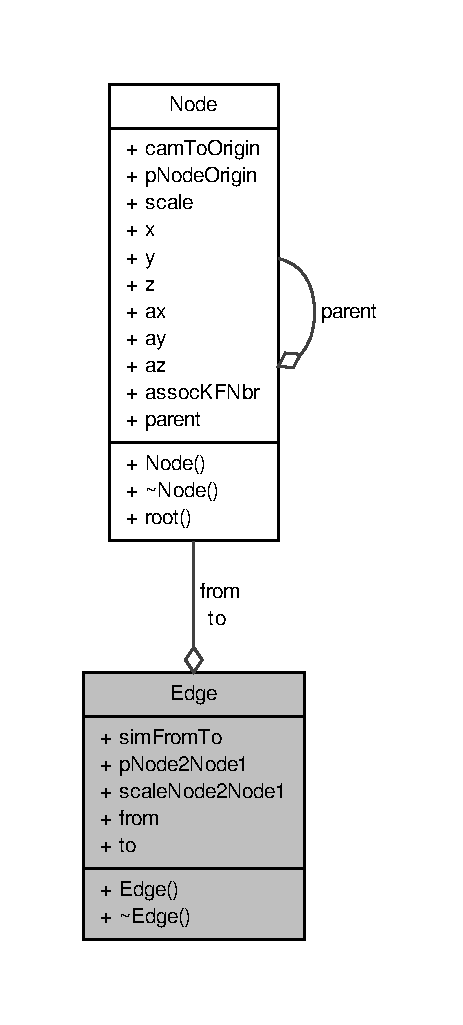
\includegraphics[width=222pt]{classEdge__coll__graph}
\end{center}
\end{figure}
\subsection*{\-Public \-Member \-Functions}
\begin{DoxyCompactItemize}
\item 
\hyperlink{classEdge_a3106b11d60125009dbf7a738ce540fdf}{\-Edge} ()
\item 
\hyperlink{classEdge_a2f37b72f044427961d6730943daf10e0}{$\sim$\-Edge} ()
\end{DoxyCompactItemize}
\subsection*{\-Public \-Attributes}
\begin{DoxyCompactItemize}
\item 
float \hyperlink{classEdge_ac612d1d9593c51a94b24d4c602289e3d}{sim\-From\-To} \mbox{[}7\mbox{]}
\item 
\-Eigen\-::\-Matrix4f \hyperlink{classEdge_af0f27040f602b9c69ca1f961d9d5fb6c}{p\-Node2\-Node1}
\item 
float \hyperlink{classEdge_a7c93e09bb582c2044e1db881bd55627b}{scale\-Node2\-Node1}
\item 
\hyperlink{classNode}{\-Node} $\ast$ \hyperlink{classEdge_ab333b0c09db333edb0b19b115893b736}{from}
\item 
\hyperlink{classNode}{\-Node} $\ast$ \hyperlink{classEdge_a7a09acfaaccec8241ee0c00a3b5c1354}{to}
\end{DoxyCompactItemize}


\subsection{\-Detailed \-Description}


\-Definition at line 31 of file \-Pose\-Graph.\-h.



\subsection{\-Constructor \& \-Destructor \-Documentation}
\hypertarget{classEdge_a3106b11d60125009dbf7a738ce540fdf}{\index{\-Edge@{\-Edge}!\-Edge@{\-Edge}}
\index{\-Edge@{\-Edge}!Edge@{\-Edge}}
\subsubsection[{\-Edge}]{\setlength{\rightskip}{0pt plus 5cm}{\bf \-Edge\-::\-Edge} (
\begin{DoxyParamCaption}
{}
\end{DoxyParamCaption}
)}}\label{classEdge_a3106b11d60125009dbf7a738ce540fdf}


\-Definition at line 24 of file \-Pose\-Graph.\-cpp.


\begin{DoxyCode}
           {
        // quat.x() = trafoFloat[0]; quat.y() = trafoFloat[1]; quat.z() =
       trafoFloat[2]; quat.w() = trafoFloat[3];
        // transl.x() = trafoFloat[4]; transl.y() = trafoFloat[5]; transl.z() =
       trafoFloat[6];
        for(int i=0; i<7; ++i) {
                simFromTo[i] = 0.0;
                if(i==3) {
                        simFromTo[i] = 1.0;
                }
        }
        pNode2Node1 = Eigen::Matrix4f::Identity(4,4);
        scaleNode2Node1 = 1.0;

        from = NULL;
        to = NULL;
}
\end{DoxyCode}
\hypertarget{classEdge_a2f37b72f044427961d6730943daf10e0}{\index{\-Edge@{\-Edge}!$\sim$\-Edge@{$\sim$\-Edge}}
\index{$\sim$\-Edge@{$\sim$\-Edge}!Edge@{\-Edge}}
\subsubsection[{$\sim$\-Edge}]{\setlength{\rightskip}{0pt plus 5cm}{\bf \-Edge\-::$\sim$\-Edge} (
\begin{DoxyParamCaption}
{}
\end{DoxyParamCaption}
)}}\label{classEdge_a2f37b72f044427961d6730943daf10e0}


\-Definition at line 40 of file \-Pose\-Graph.\-cpp.


\begin{DoxyCode}
{}
\end{DoxyCode}


\subsection{\-Member \-Data \-Documentation}
\hypertarget{classEdge_ab333b0c09db333edb0b19b115893b736}{\index{\-Edge@{\-Edge}!from@{from}}
\index{from@{from}!Edge@{\-Edge}}
\subsubsection[{from}]{\setlength{\rightskip}{0pt plus 5cm}{\bf \-Node}$\ast$ {\bf \-Edge\-::from}}}\label{classEdge_ab333b0c09db333edb0b19b115893b736}


\-Definition at line 39 of file \-Pose\-Graph.\-h.

\hypertarget{classEdge_af0f27040f602b9c69ca1f961d9d5fb6c}{\index{\-Edge@{\-Edge}!p\-Node2\-Node1@{p\-Node2\-Node1}}
\index{p\-Node2\-Node1@{p\-Node2\-Node1}!Edge@{\-Edge}}
\subsubsection[{p\-Node2\-Node1}]{\setlength{\rightskip}{0pt plus 5cm}\-Eigen\-::\-Matrix4f {\bf \-Edge\-::p\-Node2\-Node1}}}\label{classEdge_af0f27040f602b9c69ca1f961d9d5fb6c}


\-Definition at line 36 of file \-Pose\-Graph.\-h.

\hypertarget{classEdge_a7c93e09bb582c2044e1db881bd55627b}{\index{\-Edge@{\-Edge}!scale\-Node2\-Node1@{scale\-Node2\-Node1}}
\index{scale\-Node2\-Node1@{scale\-Node2\-Node1}!Edge@{\-Edge}}
\subsubsection[{scale\-Node2\-Node1}]{\setlength{\rightskip}{0pt plus 5cm}float {\bf \-Edge\-::scale\-Node2\-Node1}}}\label{classEdge_a7c93e09bb582c2044e1db881bd55627b}


\-Definition at line 37 of file \-Pose\-Graph.\-h.

\hypertarget{classEdge_ac612d1d9593c51a94b24d4c602289e3d}{\index{\-Edge@{\-Edge}!sim\-From\-To@{sim\-From\-To}}
\index{sim\-From\-To@{sim\-From\-To}!Edge@{\-Edge}}
\subsubsection[{sim\-From\-To}]{\setlength{\rightskip}{0pt plus 5cm}float {\bf \-Edge\-::sim\-From\-To}\mbox{[}7\mbox{]}}}\label{classEdge_ac612d1d9593c51a94b24d4c602289e3d}


\-Definition at line 35 of file \-Pose\-Graph.\-h.

\hypertarget{classEdge_a7a09acfaaccec8241ee0c00a3b5c1354}{\index{\-Edge@{\-Edge}!to@{to}}
\index{to@{to}!Edge@{\-Edge}}
\subsubsection[{to}]{\setlength{\rightskip}{0pt plus 5cm}{\bf \-Node} $\ast$ {\bf \-Edge\-::to}}}\label{classEdge_a7a09acfaaccec8241ee0c00a3b5c1354}


\-Definition at line 39 of file \-Pose\-Graph.\-h.



\-The documentation for this class was generated from the following files\-:\begin{DoxyCompactItemize}
\item 
\hyperlink{PoseGraph_8h}{\-Pose\-Graph.\-h}\item 
\hyperlink{PoseGraph_8cpp}{\-Pose\-Graph.\-cpp}\end{DoxyCompactItemize}

\hypertarget{structGraphConstraint}{\section{\-Graph\-Constraint \-Struct \-Reference}
\label{structGraphConstraint}\index{\-Graph\-Constraint@{\-Graph\-Constraint}}
}


{\ttfamily \#include $<$\-Sync\-Listener.\-h$>$}

\subsection*{\-Public \-Attributes}
\begin{DoxyCompactItemize}
\item 
int \hyperlink{structGraphConstraint_a6aa031743203b4691eb90397e6b2b27d}{from}
\item 
int \hyperlink{structGraphConstraint_aacbe0ea6278c9005bec666c1df276912}{to}
\item 
float \hyperlink{structGraphConstraint_a3d6dbef26111f030919673ba40fed465}{err}
\end{DoxyCompactItemize}


\subsection{\-Detailed \-Description}


\-Definition at line 54 of file \-Sync\-Listener.\-h.



\subsection{\-Member \-Data \-Documentation}
\hypertarget{structGraphConstraint_a3d6dbef26111f030919673ba40fed465}{\index{\-Graph\-Constraint@{\-Graph\-Constraint}!err@{err}}
\index{err@{err}!GraphConstraint@{\-Graph\-Constraint}}
\subsubsection[{err}]{\setlength{\rightskip}{0pt plus 5cm}float {\bf \-Graph\-Constraint\-::err}}}\label{structGraphConstraint_a3d6dbef26111f030919673ba40fed465}


\-Definition at line 58 of file \-Sync\-Listener.\-h.

\hypertarget{structGraphConstraint_a6aa031743203b4691eb90397e6b2b27d}{\index{\-Graph\-Constraint@{\-Graph\-Constraint}!from@{from}}
\index{from@{from}!GraphConstraint@{\-Graph\-Constraint}}
\subsubsection[{from}]{\setlength{\rightskip}{0pt plus 5cm}int {\bf \-Graph\-Constraint\-::from}}}\label{structGraphConstraint_a6aa031743203b4691eb90397e6b2b27d}


\-Definition at line 56 of file \-Sync\-Listener.\-h.

\hypertarget{structGraphConstraint_aacbe0ea6278c9005bec666c1df276912}{\index{\-Graph\-Constraint@{\-Graph\-Constraint}!to@{to}}
\index{to@{to}!GraphConstraint@{\-Graph\-Constraint}}
\subsubsection[{to}]{\setlength{\rightskip}{0pt plus 5cm}int {\bf \-Graph\-Constraint\-::to}}}\label{structGraphConstraint_aacbe0ea6278c9005bec666c1df276912}


\-Definition at line 57 of file \-Sync\-Listener.\-h.



\-The documentation for this struct was generated from the following file\-:\begin{DoxyCompactItemize}
\item 
\hyperlink{SyncListener_8h}{\-Sync\-Listener.\-h}\end{DoxyCompactItemize}

\hypertarget{structGraphFramePose}{\section{\-Graph\-Frame\-Pose \-Struct \-Reference}
\label{structGraphFramePose}\index{\-Graph\-Frame\-Pose@{\-Graph\-Frame\-Pose}}
}


{\ttfamily \#include $<$\-Sync\-Listener.\-h$>$}

\subsection*{\-Public \-Attributes}
\begin{DoxyCompactItemize}
\item 
int \hyperlink{structGraphFramePose_af26009f41d2371939bb44dfde237e328}{id}
\item 
float \hyperlink{structGraphFramePose_ab0c5dc065160c1baf8ee33320b3bb896}{cam\-To\-World} \mbox{[}7\mbox{]}
\end{DoxyCompactItemize}


\subsection{\-Detailed \-Description}


\-Definition at line 49 of file \-Sync\-Listener.\-h.



\subsection{\-Member \-Data \-Documentation}
\hypertarget{structGraphFramePose_ab0c5dc065160c1baf8ee33320b3bb896}{\index{\-Graph\-Frame\-Pose@{\-Graph\-Frame\-Pose}!cam\-To\-World@{cam\-To\-World}}
\index{cam\-To\-World@{cam\-To\-World}!GraphFramePose@{\-Graph\-Frame\-Pose}}
\subsubsection[{cam\-To\-World}]{\setlength{\rightskip}{0pt plus 5cm}float {\bf \-Graph\-Frame\-Pose\-::cam\-To\-World}\mbox{[}7\mbox{]}}}\label{structGraphFramePose_ab0c5dc065160c1baf8ee33320b3bb896}


\-Definition at line 51 of file \-Sync\-Listener.\-h.

\hypertarget{structGraphFramePose_af26009f41d2371939bb44dfde237e328}{\index{\-Graph\-Frame\-Pose@{\-Graph\-Frame\-Pose}!id@{id}}
\index{id@{id}!GraphFramePose@{\-Graph\-Frame\-Pose}}
\subsubsection[{id}]{\setlength{\rightskip}{0pt plus 5cm}int {\bf \-Graph\-Frame\-Pose\-::id}}}\label{structGraphFramePose_af26009f41d2371939bb44dfde237e328}


\-Definition at line 50 of file \-Sync\-Listener.\-h.



\-The documentation for this struct was generated from the following file\-:\begin{DoxyCompactItemize}
\item 
\hyperlink{SyncListener_8h}{\-Sync\-Listener.\-h}\end{DoxyCompactItemize}

\hypertarget{classHelperFcts}{\section{\-Helper\-Fcts \-Class \-Reference}
\label{classHelperFcts}\index{\-Helper\-Fcts@{\-Helper\-Fcts}}
}


{\ttfamily \#include $<$\-Helper\-Fcts.\-h$>$}

\subsection*{\-Public \-Member \-Functions}
\begin{DoxyCompactItemize}
\item 
\hyperlink{classHelperFcts_a2077e86e8be5241c948108f3d128659a}{\-Helper\-Fcts} ()
\item 
\hyperlink{classHelperFcts_af4bf4fc5be60e0dd14b54a308b38fee9}{$\sim$\-Helper\-Fcts} ()
\end{DoxyCompactItemize}
\subsection*{\-Static \-Public \-Member \-Functions}
\begin{DoxyCompactItemize}
\item 
static void \hyperlink{classHelperFcts_a78ecd5fc1beee4ac69e27e0a07258b50}{calc3\-D\-Pt} (\-Point2f pt2\-D, float fx, float fy, float cx, float cy, \-Mat idepth, \-Eigen\-::\-Vector3f \&pt3\-D)
\item 
static void \hyperlink{classHelperFcts_a3ebc81e09f781348d15f4f1898d7fb05}{display\-Image} (string window\-Name, \-Mat img)
\item 
static void \hyperlink{classHelperFcts_ac6ef7c94a83c9c7e79d83002528943de}{display\-Image\-K\-Pts} (string window\-Name, \-Mat img, vector$<$ \-Key\-Point $>$ k\-Pts)
\item 
static void \hyperlink{classHelperFcts_a604ec2c5d85568f3b51a08c268e9578c}{display\-Matches} (string window\-Name, \-Mat img1, \-Mat img2, vector$<$ \-Key\-Point $>$ k\-Pts1, vector$<$ \-Key\-Point $>$ k\-Pts2, vector$<$ \-D\-Match $>$ matches1to2, bool bool\-Save\-Img)
\item 
static void \hyperlink{classHelperFcts_a30131b3e45462ea3574240002efc9888}{display\-Save\-Image} (string window\-Name, \-Mat img, string name\-Incling\-Dir)
\item 
static void \hyperlink{classHelperFcts_aa8536f7744cd1ed6acba4fd7fe5fe8e8}{eigen\-Matrix4f\-To\-R\-O\-S\-Trafo\-Msg} (\-Eigen\-::\-Matrix4f trafo, tf\-::\-Transform \&trafo\-R\-O\-S\-Msg)
\item 
static void \hyperlink{classHelperFcts_ab7e012afc5fa512ff3f0961acac28f2e}{eigen\-Quat\-Transl\-Pose\-To\-R\-O\-S\-Pose} (\-Eigen\-::\-Quaternion$<$ float $>$ quat, \-Eigen\-::\-Translation$<$ float, 3 $>$ transl, geometry\-\_\-msgs\-::\-Pose\-Stamped \&pose)
\item 
static void \hyperlink{classHelperFcts_a987a1fd70323c857815e75b44dc432d9}{inv\-Quat\-Transl\-Scale} (\-Eigen\-::\-Quaternion$<$ float $>$ quat, \-Eigen\-::\-Quaternion$<$ float $>$ \&quat\-Inv, \-Eigen\-::\-Translation$<$ float, 3 $>$ transl, \-Eigen\-::\-Translation$<$ float, 3 $>$ \&transl\-Inv, float sc, float \&sc\-Inv)
\item 
static void \hyperlink{classHelperFcts_a92f54d3196a89e988323e73ebe14e106}{inv\-Trafo} (\-Eigen\-::\-Matrix4f trafo, \-Eigen\-::\-Matrix4f \&trafo\-Inv)
\item 
static void \hyperlink{classHelperFcts_ad8c1a028f297ea395c9d8239f64a74e2}{pose\-Stamped\-R\-O\-S\-To\-Matrix4f} (geometry\-\_\-msgs\-::\-Pose\-Stamped pose\-R\-O\-S, \-Eigen\-::\-Matrix4f \&pose\-Mat)
\item 
static void \hyperlink{classHelperFcts_aa89f2cb609374b9846dcc312a4d05212}{pose\-R\-O\-S\-To\-Trafo\-R\-O\-S\-Msg} (geometry\-\_\-msgs\-::\-Pose trafo, tf\-::\-Transform \&trafo\-R\-O\-S\-Msg)
\item 
static void \hyperlink{classHelperFcts_acb1b3fdb2752c224b2323a836f5d29ab}{custom\-Ransac} (vector$<$ \-Point2f $>$ matched\-Pts\-Query, vector$<$ \-Point2f $>$ matched\-Pts\-Test, int dim\-Model, int max\-Iter, float thresh\-Dist, float inl\-Ratio)
\item 
static void \hyperlink{classHelperFcts_a62a2cbe4631785fe2e85c9131153d8f6}{save\-Image} (\-Mat img, string name\-Incling\-Dir)
\item 
static void \hyperlink{classHelperFcts_a64c4237c737ffe6a9f06194d65a762bc}{save\-Matrix} (\-Mat matrix, string name\-Incling\-Dir)
\item 
static void \hyperlink{classHelperFcts_a496060ba1f925b932814bdaafde769d5}{save\-String\-To\-File} (string content, string name\-Incling\-Dir)
\item 
static void \hyperlink{classHelperFcts_a06b2c2707f3a2172820946196a282d8a}{trafo\-Float7\-Matrix4f} (float trafo\-Float\mbox{[}7\mbox{]}, \-Eigen\-::\-Matrix4f \&trafo\-Mat)
\item 
static void \hyperlink{classHelperFcts_aca9eeaf896ec92535fbef642133a73fe}{trafo\-Float7\-To\-Quat\-Transl\-Scale} (float sim\-Trafo\mbox{[}7\mbox{]}, \-Eigen\-::\-Quaternion$<$ float $>$ \&quat, \-Eigen\-::\-Translation$<$ float, 3 $>$ \&transl, float \&sc)
\item 
static void \hyperlink{classHelperFcts_a63c33b2156813b25f1034b66985984bd}{transform3\-D\-Pt} (float sim\-Trafo\mbox{[}7\mbox{]}, \-Eigen\-::\-Vector3f pt3\-D, \-Eigen\-::\-Vector3f \&pt3\-D\-Transformed)
\item 
static void \hyperlink{classHelperFcts_a9145127a1996c642db5ffbf188238108}{transform3\-D\-Pt} (\-Eigen\-::\-Matrix4f sim\-Trafo, \-Eigen\-::\-Vector3f pt3\-D, \-Eigen\-::\-Vector3f \&pt3\-D\-Transformed)
\end{DoxyCompactItemize}


\subsection{\-Detailed \-Description}


\-Definition at line 19 of file \-Helper\-Fcts.\-h.



\subsection{\-Constructor \& \-Destructor \-Documentation}
\hypertarget{classHelperFcts_a2077e86e8be5241c948108f3d128659a}{\index{\-Helper\-Fcts@{\-Helper\-Fcts}!\-Helper\-Fcts@{\-Helper\-Fcts}}
\index{\-Helper\-Fcts@{\-Helper\-Fcts}!HelperFcts@{\-Helper\-Fcts}}
\subsubsection[{\-Helper\-Fcts}]{\setlength{\rightskip}{0pt plus 5cm}{\bf \-Helper\-Fcts\-::\-Helper\-Fcts} (
\begin{DoxyParamCaption}
{}
\end{DoxyParamCaption}
)}}\label{classHelperFcts_a2077e86e8be5241c948108f3d128659a}


\-Definition at line 7 of file \-Helper\-Fcts.\-cpp.


\begin{DoxyCode}
{}
\end{DoxyCode}
\hypertarget{classHelperFcts_af4bf4fc5be60e0dd14b54a308b38fee9}{\index{\-Helper\-Fcts@{\-Helper\-Fcts}!$\sim$\-Helper\-Fcts@{$\sim$\-Helper\-Fcts}}
\index{$\sim$\-Helper\-Fcts@{$\sim$\-Helper\-Fcts}!HelperFcts@{\-Helper\-Fcts}}
\subsubsection[{$\sim$\-Helper\-Fcts}]{\setlength{\rightskip}{0pt plus 5cm}{\bf \-Helper\-Fcts\-::$\sim$\-Helper\-Fcts} (
\begin{DoxyParamCaption}
{}
\end{DoxyParamCaption}
)}}\label{classHelperFcts_af4bf4fc5be60e0dd14b54a308b38fee9}


\-Definition at line 8 of file \-Helper\-Fcts.\-cpp.


\begin{DoxyCode}
{}
\end{DoxyCode}


\subsection{\-Member \-Function \-Documentation}
\hypertarget{classHelperFcts_a78ecd5fc1beee4ac69e27e0a07258b50}{\index{\-Helper\-Fcts@{\-Helper\-Fcts}!calc3\-D\-Pt@{calc3\-D\-Pt}}
\index{calc3\-D\-Pt@{calc3\-D\-Pt}!HelperFcts@{\-Helper\-Fcts}}
\subsubsection[{calc3\-D\-Pt}]{\setlength{\rightskip}{0pt plus 5cm}void {\bf \-Helper\-Fcts\-::calc3\-D\-Pt} (
\begin{DoxyParamCaption}
\item[{\-Point2f}]{pt2\-D, }
\item[{float}]{fx, }
\item[{float}]{fy, }
\item[{float}]{cx, }
\item[{float}]{cy, }
\item[{\-Mat}]{idepth, }
\item[{\-Eigen\-::\-Vector3f \&}]{pt3\-D}
\end{DoxyParamCaption}
)\hspace{0.3cm}{\ttfamily  \mbox{[}static\mbox{]}}}}\label{classHelperFcts_a78ecd5fc1beee4ac69e27e0a07258b50}


\-Definition at line 10 of file \-Helper\-Fcts.\-cpp.


\begin{DoxyCode}
                                                                               
                                       {
        pt3D << pt2D.x*1/fx + (-cx/fx), pt2D.y*1/fy + (-cy/fy), 1.0;
        float depth = 1/idepth.at<float>(pt2D.x,pt2D.y);

        pt3D = pt3D*depth;
}
\end{DoxyCode}
\hypertarget{classHelperFcts_acb1b3fdb2752c224b2323a836f5d29ab}{\index{\-Helper\-Fcts@{\-Helper\-Fcts}!custom\-Ransac@{custom\-Ransac}}
\index{custom\-Ransac@{custom\-Ransac}!HelperFcts@{\-Helper\-Fcts}}
\subsubsection[{custom\-Ransac}]{\setlength{\rightskip}{0pt plus 5cm}static void {\bf \-Helper\-Fcts\-::custom\-Ransac} (
\begin{DoxyParamCaption}
\item[{vector$<$ \-Point2f $>$}]{matched\-Pts\-Query, }
\item[{vector$<$ \-Point2f $>$}]{matched\-Pts\-Test, }
\item[{int}]{dim\-Model, }
\item[{int}]{max\-Iter, }
\item[{float}]{thresh\-Dist, }
\item[{float}]{inl\-Ratio}
\end{DoxyParamCaption}
)\hspace{0.3cm}{\ttfamily  \mbox{[}static\mbox{]}}}}\label{classHelperFcts_acb1b3fdb2752c224b2323a836f5d29ab}
\hypertarget{classHelperFcts_a3ebc81e09f781348d15f4f1898d7fb05}{\index{\-Helper\-Fcts@{\-Helper\-Fcts}!display\-Image@{display\-Image}}
\index{display\-Image@{display\-Image}!HelperFcts@{\-Helper\-Fcts}}
\subsubsection[{display\-Image}]{\setlength{\rightskip}{0pt plus 5cm}void {\bf \-Helper\-Fcts\-::display\-Image} (
\begin{DoxyParamCaption}
\item[{string}]{window\-Name, }
\item[{\-Mat}]{img}
\end{DoxyParamCaption}
)\hspace{0.3cm}{\ttfamily  \mbox{[}static\mbox{]}}}}\label{classHelperFcts_a3ebc81e09f781348d15f4f1898d7fb05}


\-Definition at line 17 of file \-Helper\-Fcts.\-cpp.


\begin{DoxyCode}
                                                        {
    imshow(windowName, img);
    waitKey(10);
}
\end{DoxyCode}
\hypertarget{classHelperFcts_ac6ef7c94a83c9c7e79d83002528943de}{\index{\-Helper\-Fcts@{\-Helper\-Fcts}!display\-Image\-K\-Pts@{display\-Image\-K\-Pts}}
\index{display\-Image\-K\-Pts@{display\-Image\-K\-Pts}!HelperFcts@{\-Helper\-Fcts}}
\subsubsection[{display\-Image\-K\-Pts}]{\setlength{\rightskip}{0pt plus 5cm}void {\bf \-Helper\-Fcts\-::display\-Image\-K\-Pts} (
\begin{DoxyParamCaption}
\item[{string}]{window\-Name, }
\item[{\-Mat}]{img, }
\item[{vector$<$ \-Key\-Point $>$}]{k\-Pts}
\end{DoxyParamCaption}
)\hspace{0.3cm}{\ttfamily  \mbox{[}static\mbox{]}}}}\label{classHelperFcts_ac6ef7c94a83c9c7e79d83002528943de}


\-Definition at line 22 of file \-Helper\-Fcts.\-cpp.


\begin{DoxyCode}
                                                                               
          {
        Mat imgModified;
        drawKeypoints(img, kPts, imgModified);
    imshow(windowName, imgModified);
    waitKey(10);
}
\end{DoxyCode}
\hypertarget{classHelperFcts_a604ec2c5d85568f3b51a08c268e9578c}{\index{\-Helper\-Fcts@{\-Helper\-Fcts}!display\-Matches@{display\-Matches}}
\index{display\-Matches@{display\-Matches}!HelperFcts@{\-Helper\-Fcts}}
\subsubsection[{display\-Matches}]{\setlength{\rightskip}{0pt plus 5cm}void {\bf \-Helper\-Fcts\-::display\-Matches} (
\begin{DoxyParamCaption}
\item[{string}]{window\-Name, }
\item[{\-Mat}]{img1, }
\item[{\-Mat}]{img2, }
\item[{vector$<$ \-Key\-Point $>$}]{k\-Pts1, }
\item[{vector$<$ \-Key\-Point $>$}]{k\-Pts2, }
\item[{vector$<$ \-D\-Match $>$}]{matches1to2, }
\item[{bool}]{bool\-Save\-Img}
\end{DoxyParamCaption}
)\hspace{0.3cm}{\ttfamily  \mbox{[}static\mbox{]}}}}\label{classHelperFcts_a604ec2c5d85568f3b51a08c268e9578c}


\-Definition at line 29 of file \-Helper\-Fcts.\-cpp.


\begin{DoxyCode}
                                                                               
                                                                                      
          {
        Mat imgModified;
        drawMatches(img1, kPts1, img2, kPts2, matches1to2, imgModified);
    imshow(windowName, imgModified);
    waitKey(10);
    if(boolSaveImg == true) {
        HelperFcts::saveImage(imgModified,"testImgs/displayMatches.jpg");
    }
}
\end{DoxyCode}
\hypertarget{classHelperFcts_a30131b3e45462ea3574240002efc9888}{\index{\-Helper\-Fcts@{\-Helper\-Fcts}!display\-Save\-Image@{display\-Save\-Image}}
\index{display\-Save\-Image@{display\-Save\-Image}!HelperFcts@{\-Helper\-Fcts}}
\subsubsection[{display\-Save\-Image}]{\setlength{\rightskip}{0pt plus 5cm}void {\bf \-Helper\-Fcts\-::display\-Save\-Image} (
\begin{DoxyParamCaption}
\item[{string}]{window\-Name, }
\item[{\-Mat}]{img, }
\item[{string}]{name\-Incling\-Dir}
\end{DoxyParamCaption}
)\hspace{0.3cm}{\ttfamily  \mbox{[}static\mbox{]}}}}\label{classHelperFcts_a30131b3e45462ea3574240002efc9888}


\-Definition at line 39 of file \-Helper\-Fcts.\-cpp.


\begin{DoxyCode}
                                                                               
          {
    imshow(windowName, img);
    waitKey(10);
    imwrite(nameInclingDir, img);
}
\end{DoxyCode}
\hypertarget{classHelperFcts_aa8536f7744cd1ed6acba4fd7fe5fe8e8}{\index{\-Helper\-Fcts@{\-Helper\-Fcts}!eigen\-Matrix4f\-To\-R\-O\-S\-Trafo\-Msg@{eigen\-Matrix4f\-To\-R\-O\-S\-Trafo\-Msg}}
\index{eigen\-Matrix4f\-To\-R\-O\-S\-Trafo\-Msg@{eigen\-Matrix4f\-To\-R\-O\-S\-Trafo\-Msg}!HelperFcts@{\-Helper\-Fcts}}
\subsubsection[{eigen\-Matrix4f\-To\-R\-O\-S\-Trafo\-Msg}]{\setlength{\rightskip}{0pt plus 5cm}void {\bf \-Helper\-Fcts\-::eigen\-Matrix4f\-To\-R\-O\-S\-Trafo\-Msg} (
\begin{DoxyParamCaption}
\item[{\-Eigen\-::\-Matrix4f}]{trafo, }
\item[{tf\-::\-Transform \&}]{trafo\-R\-O\-S\-Msg}
\end{DoxyParamCaption}
)\hspace{0.3cm}{\ttfamily  \mbox{[}static\mbox{]}}}}\label{classHelperFcts_aa8536f7744cd1ed6acba4fd7fe5fe8e8}


\-Definition at line 45 of file \-Helper\-Fcts.\-cpp.


\begin{DoxyCode}
                                                                               
                 {
        tf::Vector3 origin( trafo(0,3), trafo(1,3), trafo(2,3) );

        Eigen::Matrix3f rot = trafo.block(0,0,3,3);
        Eigen::Quaternion<float> qEigen(rot);
        tf::Quaternion q( qEigen.x(), qEigen.y(), qEigen.z() ,qEigen.w() );
        q.normalize();

        trafoROSMsg.setOrigin(origin);
        trafoROSMsg.setRotation(q);
}
\end{DoxyCode}
\hypertarget{classHelperFcts_ab7e012afc5fa512ff3f0961acac28f2e}{\index{\-Helper\-Fcts@{\-Helper\-Fcts}!eigen\-Quat\-Transl\-Pose\-To\-R\-O\-S\-Pose@{eigen\-Quat\-Transl\-Pose\-To\-R\-O\-S\-Pose}}
\index{eigen\-Quat\-Transl\-Pose\-To\-R\-O\-S\-Pose@{eigen\-Quat\-Transl\-Pose\-To\-R\-O\-S\-Pose}!HelperFcts@{\-Helper\-Fcts}}
\subsubsection[{eigen\-Quat\-Transl\-Pose\-To\-R\-O\-S\-Pose}]{\setlength{\rightskip}{0pt plus 5cm}void {\bf \-Helper\-Fcts\-::eigen\-Quat\-Transl\-Pose\-To\-R\-O\-S\-Pose} (
\begin{DoxyParamCaption}
\item[{\-Eigen\-::\-Quaternion$<$ float $>$}]{quat, }
\item[{\-Eigen\-::\-Translation$<$ float, 3 $>$}]{transl, }
\item[{geometry\-\_\-msgs\-::\-Pose\-Stamped \&}]{pose}
\end{DoxyParamCaption}
)\hspace{0.3cm}{\ttfamily  \mbox{[}static\mbox{]}}}}\label{classHelperFcts_ab7e012afc5fa512ff3f0961acac28f2e}


\-Definition at line 57 of file \-Helper\-Fcts.\-cpp.


\begin{DoxyCode}
                                                                               
                                                                   {
        pose.pose.position.x = transl.x();
        pose.pose.position.y = transl.y();
        pose.pose.position.z = transl.z();

        quat.normalize();
        pose.pose.orientation.w = quat.w();
        pose.pose.orientation.x = quat.x();
        pose.pose.orientation.y = quat.y();
        pose.pose.orientation.z = quat.z();
}
\end{DoxyCode}
\hypertarget{classHelperFcts_a987a1fd70323c857815e75b44dc432d9}{\index{\-Helper\-Fcts@{\-Helper\-Fcts}!inv\-Quat\-Transl\-Scale@{inv\-Quat\-Transl\-Scale}}
\index{inv\-Quat\-Transl\-Scale@{inv\-Quat\-Transl\-Scale}!HelperFcts@{\-Helper\-Fcts}}
\subsubsection[{inv\-Quat\-Transl\-Scale}]{\setlength{\rightskip}{0pt plus 5cm}void {\bf \-Helper\-Fcts\-::inv\-Quat\-Transl\-Scale} (
\begin{DoxyParamCaption}
\item[{\-Eigen\-::\-Quaternion$<$ float $>$}]{quat, }
\item[{\-Eigen\-::\-Quaternion$<$ float $>$ \&}]{quat\-Inv, }
\item[{\-Eigen\-::\-Translation$<$ float, 3 $>$}]{transl, }
\item[{\-Eigen\-::\-Translation$<$ float, 3 $>$ \&}]{transl\-Inv, }
\item[{float}]{sc, }
\item[{float \&}]{sc\-Inv}
\end{DoxyParamCaption}
)\hspace{0.3cm}{\ttfamily  \mbox{[}static\mbox{]}}}}\label{classHelperFcts_a987a1fd70323c857815e75b44dc432d9}


\-Definition at line 69 of file \-Helper\-Fcts.\-cpp.


\begin{DoxyCode}
                                                                               
                                                                                      
                                          {
        quatInv = quat.inverse();

        Eigen::Vector3f translTmp1,translTmp2;
        translTmp1[0] = transl.x();
        translTmp1[1] = transl.y();
        translTmp1[2] = transl.z();
        translTmp2 = -quatInv.toRotationMatrix()*translTmp1;

        translInv.x() = translTmp2[0];
        translInv.y() = translTmp2[1];
        translInv.z() = translTmp2[2];

        scInv = 1/sc;
}
\end{DoxyCode}
\hypertarget{classHelperFcts_a92f54d3196a89e988323e73ebe14e106}{\index{\-Helper\-Fcts@{\-Helper\-Fcts}!inv\-Trafo@{inv\-Trafo}}
\index{inv\-Trafo@{inv\-Trafo}!HelperFcts@{\-Helper\-Fcts}}
\subsubsection[{inv\-Trafo}]{\setlength{\rightskip}{0pt plus 5cm}void {\bf \-Helper\-Fcts\-::inv\-Trafo} (
\begin{DoxyParamCaption}
\item[{\-Eigen\-::\-Matrix4f}]{trafo, }
\item[{\-Eigen\-::\-Matrix4f \&}]{trafo\-Inv}
\end{DoxyParamCaption}
)\hspace{0.3cm}{\ttfamily  \mbox{[}static\mbox{]}}}}\label{classHelperFcts_a92f54d3196a89e988323e73ebe14e106}


\-Definition at line 85 of file \-Helper\-Fcts.\-cpp.


\begin{DoxyCode}
                                                                       {
        trafoInv.block(0,0,3,3) = trafo.block(0,0,3,3).transpose();
        trafoInv.block(0,3,3,1) = -trafo.block(0,0,3,3).transpose()*trafo.block
      (0,3,3,1);
}
\end{DoxyCode}
\hypertarget{classHelperFcts_aa89f2cb609374b9846dcc312a4d05212}{\index{\-Helper\-Fcts@{\-Helper\-Fcts}!pose\-R\-O\-S\-To\-Trafo\-R\-O\-S\-Msg@{pose\-R\-O\-S\-To\-Trafo\-R\-O\-S\-Msg}}
\index{pose\-R\-O\-S\-To\-Trafo\-R\-O\-S\-Msg@{pose\-R\-O\-S\-To\-Trafo\-R\-O\-S\-Msg}!HelperFcts@{\-Helper\-Fcts}}
\subsubsection[{pose\-R\-O\-S\-To\-Trafo\-R\-O\-S\-Msg}]{\setlength{\rightskip}{0pt plus 5cm}void {\bf \-Helper\-Fcts\-::pose\-R\-O\-S\-To\-Trafo\-R\-O\-S\-Msg} (
\begin{DoxyParamCaption}
\item[{geometry\-\_\-msgs\-::\-Pose}]{trafo, }
\item[{tf\-::\-Transform \&}]{trafo\-R\-O\-S\-Msg}
\end{DoxyParamCaption}
)\hspace{0.3cm}{\ttfamily  \mbox{[}static\mbox{]}}}}\label{classHelperFcts_aa89f2cb609374b9846dcc312a4d05212}


\-Definition at line 104 of file \-Helper\-Fcts.\-cpp.


\begin{DoxyCode}
                                                                               
              {
        tf::Vector3 origin(trafo.position.x, trafo.position.y, trafo.position.z
      );
        tf::Quaternion q;
        q.setW(trafo.orientation.w);
        q.setX(trafo.orientation.x);
        q.setY(trafo.orientation.y);
        q.setZ(trafo.orientation.z);
        q.normalize();

        trafoROSMsg.setOrigin(origin);
        trafoROSMsg.setRotation(q);
}
\end{DoxyCode}
\hypertarget{classHelperFcts_ad8c1a028f297ea395c9d8239f64a74e2}{\index{\-Helper\-Fcts@{\-Helper\-Fcts}!pose\-Stamped\-R\-O\-S\-To\-Matrix4f@{pose\-Stamped\-R\-O\-S\-To\-Matrix4f}}
\index{pose\-Stamped\-R\-O\-S\-To\-Matrix4f@{pose\-Stamped\-R\-O\-S\-To\-Matrix4f}!HelperFcts@{\-Helper\-Fcts}}
\subsubsection[{pose\-Stamped\-R\-O\-S\-To\-Matrix4f}]{\setlength{\rightskip}{0pt plus 5cm}void {\bf \-Helper\-Fcts\-::pose\-Stamped\-R\-O\-S\-To\-Matrix4f} (
\begin{DoxyParamCaption}
\item[{geometry\-\_\-msgs\-::\-Pose\-Stamped}]{pose\-R\-O\-S, }
\item[{\-Eigen\-::\-Matrix4f \&}]{pose\-Mat}
\end{DoxyParamCaption}
)\hspace{0.3cm}{\ttfamily  \mbox{[}static\mbox{]}}}}\label{classHelperFcts_ad8c1a028f297ea395c9d8239f64a74e2}


\-Definition at line 90 of file \-Helper\-Fcts.\-cpp.


\begin{DoxyCode}
                                                                               
                          {
        poseMat.setIdentity(4,4);

        Eigen::Quaternion<float> quat;
        quat.w() = poseROS.pose.orientation.w;
        quat.x() = poseROS.pose.orientation.x;
        quat.y() = poseROS.pose.orientation.y;
        quat.z() = poseROS.pose.orientation.z;


        poseMat.block(0,0,3,3) = quat.toRotationMatrix();
        poseMat.block(0,3,3,1) << poseROS.pose.position.x, poseROS.pose.
      position.y, poseROS.pose.position.z;
}
\end{DoxyCode}
\hypertarget{classHelperFcts_a62a2cbe4631785fe2e85c9131153d8f6}{\index{\-Helper\-Fcts@{\-Helper\-Fcts}!save\-Image@{save\-Image}}
\index{save\-Image@{save\-Image}!HelperFcts@{\-Helper\-Fcts}}
\subsubsection[{save\-Image}]{\setlength{\rightskip}{0pt plus 5cm}void {\bf \-Helper\-Fcts\-::save\-Image} (
\begin{DoxyParamCaption}
\item[{\-Mat}]{img, }
\item[{string}]{name\-Incling\-Dir}
\end{DoxyParamCaption}
)\hspace{0.3cm}{\ttfamily  \mbox{[}static\mbox{]}}}}\label{classHelperFcts_a62a2cbe4631785fe2e85c9131153d8f6}


\-Definition at line 117 of file \-Helper\-Fcts.\-cpp.


\begin{DoxyCode}
                                                         {
    imwrite(nameInclingDir, img);
}
\end{DoxyCode}
\hypertarget{classHelperFcts_a64c4237c737ffe6a9f06194d65a762bc}{\index{\-Helper\-Fcts@{\-Helper\-Fcts}!save\-Matrix@{save\-Matrix}}
\index{save\-Matrix@{save\-Matrix}!HelperFcts@{\-Helper\-Fcts}}
\subsubsection[{save\-Matrix}]{\setlength{\rightskip}{0pt plus 5cm}void {\bf \-Helper\-Fcts\-::save\-Matrix} (
\begin{DoxyParamCaption}
\item[{\-Mat}]{matrix, }
\item[{string}]{name\-Incling\-Dir}
\end{DoxyParamCaption}
)\hspace{0.3cm}{\ttfamily  \mbox{[}static\mbox{]}}}}\label{classHelperFcts_a64c4237c737ffe6a9f06194d65a762bc}


\-Definition at line 121 of file \-Helper\-Fcts.\-cpp.


\begin{DoxyCode}
                                                             {
        cv::FileStorage fs(nameInclingDir, cv::FileStorage::WRITE);
        // Write to file!
        fs << "matchMatrix" << matrix;
        fs.release();
}
\end{DoxyCode}
\hypertarget{classHelperFcts_a496060ba1f925b932814bdaafde769d5}{\index{\-Helper\-Fcts@{\-Helper\-Fcts}!save\-String\-To\-File@{save\-String\-To\-File}}
\index{save\-String\-To\-File@{save\-String\-To\-File}!HelperFcts@{\-Helper\-Fcts}}
\subsubsection[{save\-String\-To\-File}]{\setlength{\rightskip}{0pt plus 5cm}void {\bf \-Helper\-Fcts\-::save\-String\-To\-File} (
\begin{DoxyParamCaption}
\item[{string}]{content, }
\item[{string}]{name\-Incling\-Dir}
\end{DoxyParamCaption}
)\hspace{0.3cm}{\ttfamily  \mbox{[}static\mbox{]}}}}\label{classHelperFcts_a496060ba1f925b932814bdaafde769d5}


\-Definition at line 128 of file \-Helper\-Fcts.\-cpp.


\begin{DoxyCode}
                                                                       {
        cv::FileStorage fs(nameInclingDir, cv::FileStorage::WRITE);
        // Write to file!
        fs << "CONTENT" << content;
        fs.release();
}
\end{DoxyCode}
\hypertarget{classHelperFcts_a06b2c2707f3a2172820946196a282d8a}{\index{\-Helper\-Fcts@{\-Helper\-Fcts}!trafo\-Float7\-Matrix4f@{trafo\-Float7\-Matrix4f}}
\index{trafo\-Float7\-Matrix4f@{trafo\-Float7\-Matrix4f}!HelperFcts@{\-Helper\-Fcts}}
\subsubsection[{trafo\-Float7\-Matrix4f}]{\setlength{\rightskip}{0pt plus 5cm}void {\bf \-Helper\-Fcts\-::trafo\-Float7\-Matrix4f} (
\begin{DoxyParamCaption}
\item[{float}]{trafo\-Float\mbox{[}7\mbox{]}, }
\item[{\-Eigen\-::\-Matrix4f \&}]{trafo\-Mat}
\end{DoxyParamCaption}
)\hspace{0.3cm}{\ttfamily  \mbox{[}static\mbox{]}}}}\label{classHelperFcts_a06b2c2707f3a2172820946196a282d8a}


\-Definition at line 135 of file \-Helper\-Fcts.\-cpp.


\begin{DoxyCode}
                                                                               
         {
        trafoMat.setIdentity(4,4);

        Eigen::Quaternion<float> quat;
        quat.x() = trafoFloat[0];
        quat.y() = trafoFloat[1];
        quat.z() = trafoFloat[2];
        quat.w() = trafoFloat[3];

        float sc = quat.norm();
        quat.normalize();

        trafoMat.block(0,0,3,3) = quat.toRotationMatrix();
        trafoMat.block(0,3,3,1) << trafoFloat[4], trafoFloat[5], trafoFloat[6];
}
\end{DoxyCode}
\hypertarget{classHelperFcts_aca9eeaf896ec92535fbef642133a73fe}{\index{\-Helper\-Fcts@{\-Helper\-Fcts}!trafo\-Float7\-To\-Quat\-Transl\-Scale@{trafo\-Float7\-To\-Quat\-Transl\-Scale}}
\index{trafo\-Float7\-To\-Quat\-Transl\-Scale@{trafo\-Float7\-To\-Quat\-Transl\-Scale}!HelperFcts@{\-Helper\-Fcts}}
\subsubsection[{trafo\-Float7\-To\-Quat\-Transl\-Scale}]{\setlength{\rightskip}{0pt plus 5cm}void {\bf \-Helper\-Fcts\-::trafo\-Float7\-To\-Quat\-Transl\-Scale} (
\begin{DoxyParamCaption}
\item[{float}]{sim\-Trafo\mbox{[}7\mbox{]}, }
\item[{\-Eigen\-::\-Quaternion$<$ float $>$ \&}]{quat, }
\item[{\-Eigen\-::\-Translation$<$ float, 3 $>$ \&}]{transl, }
\item[{float \&}]{sc}
\end{DoxyParamCaption}
)\hspace{0.3cm}{\ttfamily  \mbox{[}static\mbox{]}}}}\label{classHelperFcts_aca9eeaf896ec92535fbef642133a73fe}


\-Definition at line 151 of file \-Helper\-Fcts.\-cpp.


\begin{DoxyCode}
                                                                               
                                                                       {
        quat.x() = trafoFloat[0];
        quat.y() = trafoFloat[1];
        quat.z() = trafoFloat[2];
        quat.w() = trafoFloat[3];

        sc = quat.norm();

        quat.normalize();

        transl.x() = trafoFloat[4];
        transl.y() = trafoFloat[5];
        transl.z() = trafoFloat[6];
}
\end{DoxyCode}
\hypertarget{classHelperFcts_a63c33b2156813b25f1034b66985984bd}{\index{\-Helper\-Fcts@{\-Helper\-Fcts}!transform3\-D\-Pt@{transform3\-D\-Pt}}
\index{transform3\-D\-Pt@{transform3\-D\-Pt}!HelperFcts@{\-Helper\-Fcts}}
\subsubsection[{transform3\-D\-Pt}]{\setlength{\rightskip}{0pt plus 5cm}void {\bf \-Helper\-Fcts\-::transform3\-D\-Pt} (
\begin{DoxyParamCaption}
\item[{float}]{sim\-Trafo\mbox{[}7\mbox{]}, }
\item[{\-Eigen\-::\-Vector3f}]{pt3\-D, }
\item[{\-Eigen\-::\-Vector3f \&}]{pt3\-D\-Transformed}
\end{DoxyParamCaption}
)\hspace{0.3cm}{\ttfamily  \mbox{[}static\mbox{]}}}}\label{classHelperFcts_a63c33b2156813b25f1034b66985984bd}


\-Definition at line 166 of file \-Helper\-Fcts.\-cpp.


\begin{DoxyCode}
                                                                               
                            {
        Eigen::Matrix4f trafoTmp(Eigen::Matrix4f::Identity(4,4));
        Eigen::Vector4f pt3DTmp;

        HelperFcts::trafoFloat7Matrix4f(simTrafo,trafoTmp);

        pt3DTmp << pt3D(0), pt3D(1), pt3D(2), 1.0;
        pt3DTmp = trafoTmp*pt3DTmp;
        pt3DTmp = pt3DTmp/pt3DTmp(3);

        pt3DTransformed(0) = pt3DTmp(0);
        pt3DTransformed(1) = pt3DTmp(1);
        pt3DTransformed(2) = pt3DTmp(2);
}
\end{DoxyCode}
\hypertarget{classHelperFcts_a9145127a1996c642db5ffbf188238108}{\index{\-Helper\-Fcts@{\-Helper\-Fcts}!transform3\-D\-Pt@{transform3\-D\-Pt}}
\index{transform3\-D\-Pt@{transform3\-D\-Pt}!HelperFcts@{\-Helper\-Fcts}}
\subsubsection[{transform3\-D\-Pt}]{\setlength{\rightskip}{0pt plus 5cm}void {\bf \-Helper\-Fcts\-::transform3\-D\-Pt} (
\begin{DoxyParamCaption}
\item[{\-Eigen\-::\-Matrix4f}]{sim\-Trafo, }
\item[{\-Eigen\-::\-Vector3f}]{pt3\-D, }
\item[{\-Eigen\-::\-Vector3f \&}]{pt3\-D\-Transformed}
\end{DoxyParamCaption}
)\hspace{0.3cm}{\ttfamily  \mbox{[}static\mbox{]}}}}\label{classHelperFcts_a9145127a1996c642db5ffbf188238108}


\-Definition at line 181 of file \-Helper\-Fcts.\-cpp.


\begin{DoxyCode}
                                                                               
                                 {
        Eigen::Vector4f pt3DTmp;

        pt3DTmp << pt3D(0), pt3D(1), pt3D(2), 1.0;
        pt3DTmp = simTrafo*pt3DTmp;
        pt3DTmp = pt3DTmp/pt3DTmp(3);

        pt3DTransformed(0) = pt3DTmp(0);
        pt3DTransformed(1) = pt3DTmp(1);
        pt3DTransformed(2) = pt3DTmp(2);
}
\end{DoxyCode}


\-The documentation for this class was generated from the following files\-:\begin{DoxyCompactItemize}
\item 
\hyperlink{HelperFcts_8h}{\-Helper\-Fcts.\-h}\item 
\hyperlink{HelperFcts_8cpp}{\-Helper\-Fcts.\-cpp}\end{DoxyCompactItemize}

\hypertarget{structInputPointDense}{\section{\-Input\-Point\-Dense \-Struct \-Reference}
\label{structInputPointDense}\index{\-Input\-Point\-Dense@{\-Input\-Point\-Dense}}
}


{\ttfamily \#include $<$\-Sync\-Listener.\-h$>$}

\subsection*{\-Public \-Attributes}
\begin{DoxyCompactItemize}
\item 
float \hyperlink{structInputPointDense_ac719189837460d806d6748847502a7ba}{idepth}
\item 
float \hyperlink{structInputPointDense_adb860b5e78f47b2d7e073559e725dda4}{idepth\-\_\-var}
\item 
uchar \hyperlink{structInputPointDense_afa5a25bb99b8216f729dc8b1876248ff}{color} \mbox{[}4\mbox{]}
\end{DoxyCompactItemize}


\subsection{\-Detailed \-Description}


\-Definition at line 42 of file \-Sync\-Listener.\-h.



\subsection{\-Member \-Data \-Documentation}
\hypertarget{structInputPointDense_afa5a25bb99b8216f729dc8b1876248ff}{\index{\-Input\-Point\-Dense@{\-Input\-Point\-Dense}!color@{color}}
\index{color@{color}!InputPointDense@{\-Input\-Point\-Dense}}
\subsubsection[{color}]{\setlength{\rightskip}{0pt plus 5cm}uchar {\bf \-Input\-Point\-Dense\-::color}\mbox{[}4\mbox{]}}}\label{structInputPointDense_afa5a25bb99b8216f729dc8b1876248ff}


\-Definition at line 45 of file \-Sync\-Listener.\-h.

\hypertarget{structInputPointDense_ac719189837460d806d6748847502a7ba}{\index{\-Input\-Point\-Dense@{\-Input\-Point\-Dense}!idepth@{idepth}}
\index{idepth@{idepth}!InputPointDense@{\-Input\-Point\-Dense}}
\subsubsection[{idepth}]{\setlength{\rightskip}{0pt plus 5cm}float {\bf \-Input\-Point\-Dense\-::idepth}}}\label{structInputPointDense_ac719189837460d806d6748847502a7ba}


\-Definition at line 43 of file \-Sync\-Listener.\-h.

\hypertarget{structInputPointDense_adb860b5e78f47b2d7e073559e725dda4}{\index{\-Input\-Point\-Dense@{\-Input\-Point\-Dense}!idepth\-\_\-var@{idepth\-\_\-var}}
\index{idepth\-\_\-var@{idepth\-\_\-var}!InputPointDense@{\-Input\-Point\-Dense}}
\subsubsection[{idepth\-\_\-var}]{\setlength{\rightskip}{0pt plus 5cm}float {\bf \-Input\-Point\-Dense\-::idepth\-\_\-var}}}\label{structInputPointDense_adb860b5e78f47b2d7e073559e725dda4}


\-Definition at line 44 of file \-Sync\-Listener.\-h.



\-The documentation for this struct was generated from the following file\-:\begin{DoxyCompactItemize}
\item 
\hyperlink{SyncListener_8h}{\-Sync\-Listener.\-h}\end{DoxyCompactItemize}

\hypertarget{classKalmanFilterScale}{\section{\-Kalman\-Filter\-Scale \-Class \-Reference}
\label{classKalmanFilterScale}\index{\-Kalman\-Filter\-Scale@{\-Kalman\-Filter\-Scale}}
}


{\ttfamily \#include $<$\-Kalman\-Filter\-Scale.\-h$>$}

\subsection*{\-Public \-Member \-Functions}
\begin{DoxyCompactItemize}
\item 
\hyperlink{classKalmanFilterScale_a2ddb2f510c2103920578bc51eb68574a}{\-Kalman\-Filter\-Scale} ()
\item 
\hyperlink{classKalmanFilterScale_a8ef5be565bd60a2027281473aecb7165}{$\sim$\-Kalman\-Filter\-Scale} ()
\end{DoxyCompactItemize}
\subsection*{\-Protected \-Member \-Functions}
\begin{DoxyCompactItemize}
\item 
void \hyperlink{classKalmanFilterScale_a2f543d979f7bedf714a4c6c6d0415a80}{make\-A} ()
\item 
void \hyperlink{classKalmanFilterScale_a9886fe7b723b1fe52a1b2fb09173cd6a}{make\-H} ()
\item 
void \hyperlink{classKalmanFilterScale_a5a305054267cfa4fb024551fe7bee7cc}{make\-V} ()
\item 
void \hyperlink{classKalmanFilterScale_aeb8f6250967beb55f4866e52fc6fe23d}{make\-R} ()
\item 
void \hyperlink{classKalmanFilterScale_a4f39209d09cada363a3848b3692eb0a1}{make\-W} ()
\item 
void \hyperlink{classKalmanFilterScale_a63d9966037b59c269bf86cf7254d4cb3}{make\-Q} ()
\item 
void \hyperlink{classKalmanFilterScale_a374bdda07afcf771760e0c4eda59de36}{make\-Process} ()
\item 
void \hyperlink{classKalmanFilterScale_aa34bc5ba7de5485d08583df61a057878}{make\-Measure} ()
\end{DoxyCompactItemize}


\subsection{\-Detailed \-Description}


\-Definition at line 8 of file \-Kalman\-Filter\-Scale.\-h.



\subsection{\-Constructor \& \-Destructor \-Documentation}
\hypertarget{classKalmanFilterScale_a2ddb2f510c2103920578bc51eb68574a}{\index{\-Kalman\-Filter\-Scale@{\-Kalman\-Filter\-Scale}!\-Kalman\-Filter\-Scale@{\-Kalman\-Filter\-Scale}}
\index{\-Kalman\-Filter\-Scale@{\-Kalman\-Filter\-Scale}!KalmanFilterScale@{\-Kalman\-Filter\-Scale}}
\subsubsection[{\-Kalman\-Filter\-Scale}]{\setlength{\rightskip}{0pt plus 5cm}{\bf \-Kalman\-Filter\-Scale\-::\-Kalman\-Filter\-Scale} (
\begin{DoxyParamCaption}
{}
\end{DoxyParamCaption}
)}}\label{classKalmanFilterScale_a2ddb2f510c2103920578bc51eb68574a}


\-Definition at line 3 of file \-Kalman\-Filter\-Scale.\-cpp.


\begin{DoxyCode}
                                     {
        setDim(1, 0, 1, 3, 3); // dim states n, dim inputs nu, dim process
       noise nw, dim measurements m, dim measurement noise nv
}
\end{DoxyCode}
\hypertarget{classKalmanFilterScale_a8ef5be565bd60a2027281473aecb7165}{\index{\-Kalman\-Filter\-Scale@{\-Kalman\-Filter\-Scale}!$\sim$\-Kalman\-Filter\-Scale@{$\sim$\-Kalman\-Filter\-Scale}}
\index{$\sim$\-Kalman\-Filter\-Scale@{$\sim$\-Kalman\-Filter\-Scale}!KalmanFilterScale@{\-Kalman\-Filter\-Scale}}
\subsubsection[{$\sim$\-Kalman\-Filter\-Scale}]{\setlength{\rightskip}{0pt plus 5cm}{\bf \-Kalman\-Filter\-Scale\-::$\sim$\-Kalman\-Filter\-Scale} (
\begin{DoxyParamCaption}
{}
\end{DoxyParamCaption}
)}}\label{classKalmanFilterScale_a8ef5be565bd60a2027281473aecb7165}


\-Definition at line 7 of file \-Kalman\-Filter\-Scale.\-cpp.


\begin{DoxyCode}
{}
\end{DoxyCode}


\subsection{\-Member \-Function \-Documentation}
\hypertarget{classKalmanFilterScale_a2f543d979f7bedf714a4c6c6d0415a80}{\index{\-Kalman\-Filter\-Scale@{\-Kalman\-Filter\-Scale}!make\-A@{make\-A}}
\index{make\-A@{make\-A}!KalmanFilterScale@{\-Kalman\-Filter\-Scale}}
\subsubsection[{make\-A}]{\setlength{\rightskip}{0pt plus 5cm}void {\bf \-Kalman\-Filter\-Scale\-::make\-A} (
\begin{DoxyParamCaption}
{}
\end{DoxyParamCaption}
)\hspace{0.3cm}{\ttfamily  \mbox{[}protected\mbox{]}}}}\label{classKalmanFilterScale_a2f543d979f7bedf714a4c6c6d0415a80}


\-Definition at line 23 of file \-Kalman\-Filter\-Scale.\-cpp.


\begin{DoxyCode}
                              {
        // Jacobian of process model
        A(1,1) = 1.0;
}
\end{DoxyCode}
\hypertarget{classKalmanFilterScale_a9886fe7b723b1fe52a1b2fb09173cd6a}{\index{\-Kalman\-Filter\-Scale@{\-Kalman\-Filter\-Scale}!make\-H@{make\-H}}
\index{make\-H@{make\-H}!KalmanFilterScale@{\-Kalman\-Filter\-Scale}}
\subsubsection[{make\-H}]{\setlength{\rightskip}{0pt plus 5cm}void {\bf \-Kalman\-Filter\-Scale\-::make\-H} (
\begin{DoxyParamCaption}
{}
\end{DoxyParamCaption}
)\hspace{0.3cm}{\ttfamily  \mbox{[}protected\mbox{]}}}}\label{classKalmanFilterScale_a9886fe7b723b1fe52a1b2fb09173cd6a}


\-Definition at line 28 of file \-Kalman\-Filter\-Scale.\-cpp.


\begin{DoxyCode}
                              {
        // Jacobian of measurement model
        H(1,1) = 1.0;
        H(2,1) = 1.0;
        H(3,1) = 1.0;
}
\end{DoxyCode}
\hypertarget{classKalmanFilterScale_aa34bc5ba7de5485d08583df61a057878}{\index{\-Kalman\-Filter\-Scale@{\-Kalman\-Filter\-Scale}!make\-Measure@{make\-Measure}}
\index{make\-Measure@{make\-Measure}!KalmanFilterScale@{\-Kalman\-Filter\-Scale}}
\subsubsection[{make\-Measure}]{\setlength{\rightskip}{0pt plus 5cm}void {\bf \-Kalman\-Filter\-Scale\-::make\-Measure} (
\begin{DoxyParamCaption}
{}
\end{DoxyParamCaption}
)\hspace{0.3cm}{\ttfamily  \mbox{[}protected\mbox{]}}}}\label{classKalmanFilterScale_aa34bc5ba7de5485d08583df61a057878}


\-Definition at line 16 of file \-Kalman\-Filter\-Scale.\-cpp.


\begin{DoxyCode}
                                    {
        // Measurement model
        z(1) = x(1);
        z(2) = x(1);
        z(3) = x(1);
}
\end{DoxyCode}
\hypertarget{classKalmanFilterScale_a374bdda07afcf771760e0c4eda59de36}{\index{\-Kalman\-Filter\-Scale@{\-Kalman\-Filter\-Scale}!make\-Process@{make\-Process}}
\index{make\-Process@{make\-Process}!KalmanFilterScale@{\-Kalman\-Filter\-Scale}}
\subsubsection[{make\-Process}]{\setlength{\rightskip}{0pt plus 5cm}void {\bf \-Kalman\-Filter\-Scale\-::make\-Process} (
\begin{DoxyParamCaption}
{}
\end{DoxyParamCaption}
)\hspace{0.3cm}{\ttfamily  \mbox{[}protected\mbox{]}}}}\label{classKalmanFilterScale_a374bdda07afcf771760e0c4eda59de36}


\-Definition at line 9 of file \-Kalman\-Filter\-Scale.\-cpp.


\begin{DoxyCode}
                                    {
        // Process model
        Vector x_(x.size());
        x_(1) = x(1);
        x.swap(x_);
}
\end{DoxyCode}
\hypertarget{classKalmanFilterScale_a63d9966037b59c269bf86cf7254d4cb3}{\index{\-Kalman\-Filter\-Scale@{\-Kalman\-Filter\-Scale}!make\-Q@{make\-Q}}
\index{make\-Q@{make\-Q}!KalmanFilterScale@{\-Kalman\-Filter\-Scale}}
\subsubsection[{make\-Q}]{\setlength{\rightskip}{0pt plus 5cm}void {\bf \-Kalman\-Filter\-Scale\-::make\-Q} (
\begin{DoxyParamCaption}
{}
\end{DoxyParamCaption}
)\hspace{0.3cm}{\ttfamily  \mbox{[}protected\mbox{]}}}}\label{classKalmanFilterScale_a63d9966037b59c269bf86cf7254d4cb3}


\-Definition at line 50 of file \-Kalman\-Filter\-Scale.\-cpp.


\begin{DoxyCode}
                              {
        // Covaricane of process noise
        Q(1,1) = 1.0;
}
\end{DoxyCode}
\hypertarget{classKalmanFilterScale_aeb8f6250967beb55f4866e52fc6fe23d}{\index{\-Kalman\-Filter\-Scale@{\-Kalman\-Filter\-Scale}!make\-R@{make\-R}}
\index{make\-R@{make\-R}!KalmanFilterScale@{\-Kalman\-Filter\-Scale}}
\subsubsection[{make\-R}]{\setlength{\rightskip}{0pt plus 5cm}void {\bf \-Kalman\-Filter\-Scale\-::make\-R} (
\begin{DoxyParamCaption}
{}
\end{DoxyParamCaption}
)\hspace{0.3cm}{\ttfamily  \mbox{[}protected\mbox{]}}}}\label{classKalmanFilterScale_aeb8f6250967beb55f4866e52fc6fe23d}


\-Definition at line 55 of file \-Kalman\-Filter\-Scale.\-cpp.


\begin{DoxyCode}
                              {
        // Covaricane of measurement noise
        R(1,1) = 1.0;
        R(2,2) = 1.0;
        R(3,3) = 1.0;

        R(2,1) = R(3,1) =
                        R(1,2) = R(3,2) =
                        R(1,3) = R(2,3) = 0.0;
}
\end{DoxyCode}
\hypertarget{classKalmanFilterScale_a5a305054267cfa4fb024551fe7bee7cc}{\index{\-Kalman\-Filter\-Scale@{\-Kalman\-Filter\-Scale}!make\-V@{make\-V}}
\index{make\-V@{make\-V}!KalmanFilterScale@{\-Kalman\-Filter\-Scale}}
\subsubsection[{make\-V}]{\setlength{\rightskip}{0pt plus 5cm}void {\bf \-Kalman\-Filter\-Scale\-::make\-V} (
\begin{DoxyParamCaption}
{}
\end{DoxyParamCaption}
)\hspace{0.3cm}{\ttfamily  \mbox{[}protected\mbox{]}}}}\label{classKalmanFilterScale_a5a305054267cfa4fb024551fe7bee7cc}


\-Definition at line 40 of file \-Kalman\-Filter\-Scale.\-cpp.


\begin{DoxyCode}
                              {
        // Jacobian of Measurement noise
        V(1,1) = 1.0;
        V(2,2) = 1.0;
        V(3,3) = 1.0;
        V(2,1) = V(3,1) =
                        V(1,2) = V(3,2) =
                        V(1,3) = V(2,3) = 0.0;
}
\end{DoxyCode}
\hypertarget{classKalmanFilterScale_a4f39209d09cada363a3848b3692eb0a1}{\index{\-Kalman\-Filter\-Scale@{\-Kalman\-Filter\-Scale}!make\-W@{make\-W}}
\index{make\-W@{make\-W}!KalmanFilterScale@{\-Kalman\-Filter\-Scale}}
\subsubsection[{make\-W}]{\setlength{\rightskip}{0pt plus 5cm}void {\bf \-Kalman\-Filter\-Scale\-::make\-W} (
\begin{DoxyParamCaption}
{}
\end{DoxyParamCaption}
)\hspace{0.3cm}{\ttfamily  \mbox{[}protected\mbox{]}}}}\label{classKalmanFilterScale_a4f39209d09cada363a3848b3692eb0a1}


\-Definition at line 35 of file \-Kalman\-Filter\-Scale.\-cpp.


\begin{DoxyCode}
                              {
        // Jacobian of process noise
        W(1,1) = 1.0;
}
\end{DoxyCode}


\-The documentation for this class was generated from the following files\-:\begin{DoxyCompactItemize}
\item 
\hyperlink{KalmanFilterScale_8h}{\-Kalman\-Filter\-Scale.\-h}\item 
\hyperlink{KalmanFilterScale_8cpp}{\-Kalman\-Filter\-Scale.\-cpp}\end{DoxyCompactItemize}

\hypertarget{structkeyFrame}{\section{key\-Frame \-Struct \-Reference}
\label{structkeyFrame}\index{key\-Frame@{key\-Frame}}
}


{\ttfamily \#include $<$\-Central\-Storage.\-h$>$}

\subsection*{\-Public \-Attributes}
\begin{DoxyCompactItemize}
\item 
\-Mat \hyperlink{structkeyFrame_a59576f76e321ecb82062edc5c7bc08fe}{img}
\item 
\-Mat \hyperlink{structkeyFrame_a12f22700cfe3b70f3a5e9f577503baf7}{bow\-Descriptor}
\item 
\-Mat \hyperlink{structkeyFrame_ac952ad626e928e521c6663e611820dac}{idepth}
\item 
\-Mat \hyperlink{structkeyFrame_a3b7c27c0435f84c12a86c00e22cfaa81}{idepth\-Var}
\item 
int \hyperlink{structkeyFrame_a3d8de485d4a812bf9dd92298ab4e1664}{r\-I\-D}
\item 
int \hyperlink{structkeyFrame_a8bbbb8e728fff6f1ee05bd8c4f846099}{f\-I\-D}
\item 
int \hyperlink{structkeyFrame_a0cf94e5999249fd9697daba9202800fe}{lsd\-S\-L\-A\-M\-I\-D}
\item 
int \hyperlink{structkeyFrame_a7c120296453059ee5b9ab853910e2c46}{width}
\item 
int \hyperlink{structkeyFrame_aa4b6b580b1cab2933803379a9fce0e0d}{height}
\item 
image\-\_\-geometry\-::\-Pinhole\-Camera\-Model \hyperlink{structkeyFrame_a61d24aeadcc9cfda14b6e99447a7971c}{cam\-Model}
\item 
float \hyperlink{structkeyFrame_a145d6d5ab1e2da4d59d34000152111cd}{fx}
\item 
float \hyperlink{structkeyFrame_a48af06b30b2f6f5a73e61afddb7ea0c4}{fy}
\item 
float \hyperlink{structkeyFrame_a237a54d29c13a64b8a3d4a597ab061c5}{cx}
\item 
float \hyperlink{structkeyFrame_ac9d3a851908cfd7587fb3e7859087e5d}{cy}
\item 
vector$<$ \-Key\-Point $>$ \hyperlink{structkeyFrame_a420102716b1d90f44af48de225f241ba}{\-K\-Pts}
\item 
float \hyperlink{structkeyFrame_a6fe79b13fb7e8e5d3b1719fa35ae7afd}{cam\-To\-Robot} \mbox{[}7\mbox{]}
\end{DoxyCompactItemize}


\subsection{\-Detailed \-Description}
\-Structure containing all information concerning to one \-Frame 

\-Definition at line 50 of file \-Central\-Storage.\-h.



\subsection{\-Member \-Data \-Documentation}
\hypertarget{structkeyFrame_a12f22700cfe3b70f3a5e9f577503baf7}{\index{key\-Frame@{key\-Frame}!bow\-Descriptor@{bow\-Descriptor}}
\index{bow\-Descriptor@{bow\-Descriptor}!keyFrame@{key\-Frame}}
\subsubsection[{bow\-Descriptor}]{\setlength{\rightskip}{0pt plus 5cm}\-Mat {\bf key\-Frame\-::bow\-Descriptor}}}\label{structkeyFrame_a12f22700cfe3b70f3a5e9f577503baf7}


\-Definition at line 53 of file \-Central\-Storage.\-h.

\hypertarget{structkeyFrame_a61d24aeadcc9cfda14b6e99447a7971c}{\index{key\-Frame@{key\-Frame}!cam\-Model@{cam\-Model}}
\index{cam\-Model@{cam\-Model}!keyFrame@{key\-Frame}}
\subsubsection[{cam\-Model}]{\setlength{\rightskip}{0pt plus 5cm}image\-\_\-geometry\-::\-Pinhole\-Camera\-Model {\bf key\-Frame\-::cam\-Model}}}\label{structkeyFrame_a61d24aeadcc9cfda14b6e99447a7971c}


\-Definition at line 63 of file \-Central\-Storage.\-h.

\hypertarget{structkeyFrame_a6fe79b13fb7e8e5d3b1719fa35ae7afd}{\index{key\-Frame@{key\-Frame}!cam\-To\-Robot@{cam\-To\-Robot}}
\index{cam\-To\-Robot@{cam\-To\-Robot}!keyFrame@{key\-Frame}}
\subsubsection[{cam\-To\-Robot}]{\setlength{\rightskip}{0pt plus 5cm}float {\bf key\-Frame\-::cam\-To\-Robot}\mbox{[}7\mbox{]}}}\label{structkeyFrame_a6fe79b13fb7e8e5d3b1719fa35ae7afd}


\-Definition at line 70 of file \-Central\-Storage.\-h.

\hypertarget{structkeyFrame_a237a54d29c13a64b8a3d4a597ab061c5}{\index{key\-Frame@{key\-Frame}!cx@{cx}}
\index{cx@{cx}!keyFrame@{key\-Frame}}
\subsubsection[{cx}]{\setlength{\rightskip}{0pt plus 5cm}float {\bf key\-Frame\-::cx}}}\label{structkeyFrame_a237a54d29c13a64b8a3d4a597ab061c5}


\-Definition at line 64 of file \-Central\-Storage.\-h.

\hypertarget{structkeyFrame_ac9d3a851908cfd7587fb3e7859087e5d}{\index{key\-Frame@{key\-Frame}!cy@{cy}}
\index{cy@{cy}!keyFrame@{key\-Frame}}
\subsubsection[{cy}]{\setlength{\rightskip}{0pt plus 5cm}float {\bf key\-Frame\-::cy}}}\label{structkeyFrame_ac9d3a851908cfd7587fb3e7859087e5d}


\-Definition at line 64 of file \-Central\-Storage.\-h.

\hypertarget{structkeyFrame_a8bbbb8e728fff6f1ee05bd8c4f846099}{\index{key\-Frame@{key\-Frame}!f\-I\-D@{f\-I\-D}}
\index{f\-I\-D@{f\-I\-D}!keyFrame@{key\-Frame}}
\subsubsection[{f\-I\-D}]{\setlength{\rightskip}{0pt plus 5cm}int {\bf key\-Frame\-::f\-I\-D}}}\label{structkeyFrame_a8bbbb8e728fff6f1ee05bd8c4f846099}


\-Definition at line 60 of file \-Central\-Storage.\-h.

\hypertarget{structkeyFrame_a145d6d5ab1e2da4d59d34000152111cd}{\index{key\-Frame@{key\-Frame}!fx@{fx}}
\index{fx@{fx}!keyFrame@{key\-Frame}}
\subsubsection[{fx}]{\setlength{\rightskip}{0pt plus 5cm}float {\bf key\-Frame\-::fx}}}\label{structkeyFrame_a145d6d5ab1e2da4d59d34000152111cd}


\-Definition at line 64 of file \-Central\-Storage.\-h.

\hypertarget{structkeyFrame_a48af06b30b2f6f5a73e61afddb7ea0c4}{\index{key\-Frame@{key\-Frame}!fy@{fy}}
\index{fy@{fy}!keyFrame@{key\-Frame}}
\subsubsection[{fy}]{\setlength{\rightskip}{0pt plus 5cm}float {\bf key\-Frame\-::fy}}}\label{structkeyFrame_a48af06b30b2f6f5a73e61afddb7ea0c4}


\-Definition at line 64 of file \-Central\-Storage.\-h.

\hypertarget{structkeyFrame_aa4b6b580b1cab2933803379a9fce0e0d}{\index{key\-Frame@{key\-Frame}!height@{height}}
\index{height@{height}!keyFrame@{key\-Frame}}
\subsubsection[{height}]{\setlength{\rightskip}{0pt plus 5cm}int {\bf key\-Frame\-::height}}}\label{structkeyFrame_aa4b6b580b1cab2933803379a9fce0e0d}


\-Definition at line 60 of file \-Central\-Storage.\-h.

\hypertarget{structkeyFrame_ac952ad626e928e521c6663e611820dac}{\index{key\-Frame@{key\-Frame}!idepth@{idepth}}
\index{idepth@{idepth}!keyFrame@{key\-Frame}}
\subsubsection[{idepth}]{\setlength{\rightskip}{0pt plus 5cm}\-Mat {\bf key\-Frame\-::idepth}}}\label{structkeyFrame_ac952ad626e928e521c6663e611820dac}


\-Definition at line 53 of file \-Central\-Storage.\-h.

\hypertarget{structkeyFrame_a3b7c27c0435f84c12a86c00e22cfaa81}{\index{key\-Frame@{key\-Frame}!idepth\-Var@{idepth\-Var}}
\index{idepth\-Var@{idepth\-Var}!keyFrame@{key\-Frame}}
\subsubsection[{idepth\-Var}]{\setlength{\rightskip}{0pt plus 5cm}\-Mat {\bf key\-Frame\-::idepth\-Var}}}\label{structkeyFrame_a3b7c27c0435f84c12a86c00e22cfaa81}


\-Definition at line 53 of file \-Central\-Storage.\-h.

\hypertarget{structkeyFrame_a59576f76e321ecb82062edc5c7bc08fe}{\index{key\-Frame@{key\-Frame}!img@{img}}
\index{img@{img}!keyFrame@{key\-Frame}}
\subsubsection[{img}]{\setlength{\rightskip}{0pt plus 5cm}\-Mat {\bf key\-Frame\-::img}}}\label{structkeyFrame_a59576f76e321ecb82062edc5c7bc08fe}


\-Definition at line 53 of file \-Central\-Storage.\-h.

\hypertarget{structkeyFrame_a420102716b1d90f44af48de225f241ba}{\index{key\-Frame@{key\-Frame}!\-K\-Pts@{\-K\-Pts}}
\index{\-K\-Pts@{\-K\-Pts}!keyFrame@{key\-Frame}}
\subsubsection[{\-K\-Pts}]{\setlength{\rightskip}{0pt plus 5cm}vector$<$\-Key\-Point$>$ {\bf key\-Frame\-::\-K\-Pts}}}\label{structkeyFrame_a420102716b1d90f44af48de225f241ba}


\-Definition at line 67 of file \-Central\-Storage.\-h.

\hypertarget{structkeyFrame_a0cf94e5999249fd9697daba9202800fe}{\index{key\-Frame@{key\-Frame}!lsd\-S\-L\-A\-M\-I\-D@{lsd\-S\-L\-A\-M\-I\-D}}
\index{lsd\-S\-L\-A\-M\-I\-D@{lsd\-S\-L\-A\-M\-I\-D}!keyFrame@{key\-Frame}}
\subsubsection[{lsd\-S\-L\-A\-M\-I\-D}]{\setlength{\rightskip}{0pt plus 5cm}int {\bf key\-Frame\-::lsd\-S\-L\-A\-M\-I\-D}}}\label{structkeyFrame_a0cf94e5999249fd9697daba9202800fe}


\-Definition at line 60 of file \-Central\-Storage.\-h.

\hypertarget{structkeyFrame_a3d8de485d4a812bf9dd92298ab4e1664}{\index{key\-Frame@{key\-Frame}!r\-I\-D@{r\-I\-D}}
\index{r\-I\-D@{r\-I\-D}!keyFrame@{key\-Frame}}
\subsubsection[{r\-I\-D}]{\setlength{\rightskip}{0pt plus 5cm}int {\bf key\-Frame\-::r\-I\-D}}}\label{structkeyFrame_a3d8de485d4a812bf9dd92298ab4e1664}


\-Definition at line 60 of file \-Central\-Storage.\-h.

\hypertarget{structkeyFrame_a7c120296453059ee5b9ab853910e2c46}{\index{key\-Frame@{key\-Frame}!width@{width}}
\index{width@{width}!keyFrame@{key\-Frame}}
\subsubsection[{width}]{\setlength{\rightskip}{0pt plus 5cm}int {\bf key\-Frame\-::width}}}\label{structkeyFrame_a7c120296453059ee5b9ab853910e2c46}


\-Definition at line 60 of file \-Central\-Storage.\-h.



\-The documentation for this struct was generated from the following file\-:\begin{DoxyCompactItemize}
\item 
\hyperlink{CentralStorage_8h}{\-Central\-Storage.\-h}\end{DoxyCompactItemize}

\hypertarget{classKeyFrameListenerTraining}{\section{\-Key\-Frame\-Listener\-Training \-Class \-Reference}
\label{classKeyFrameListenerTraining}\index{\-Key\-Frame\-Listener\-Training@{\-Key\-Frame\-Listener\-Training}}
}


\-Class listening to incoming images, each instance of the class listens to one robot -\/$>$ do training.  




{\ttfamily \#include $<$\-Key\-Frame\-Listener\-Training.\-h$>$}



\-Collaboration diagram for \-Key\-Frame\-Listener\-Training\-:\nopagebreak
\begin{figure}[H]
\begin{center}
\leavevmode
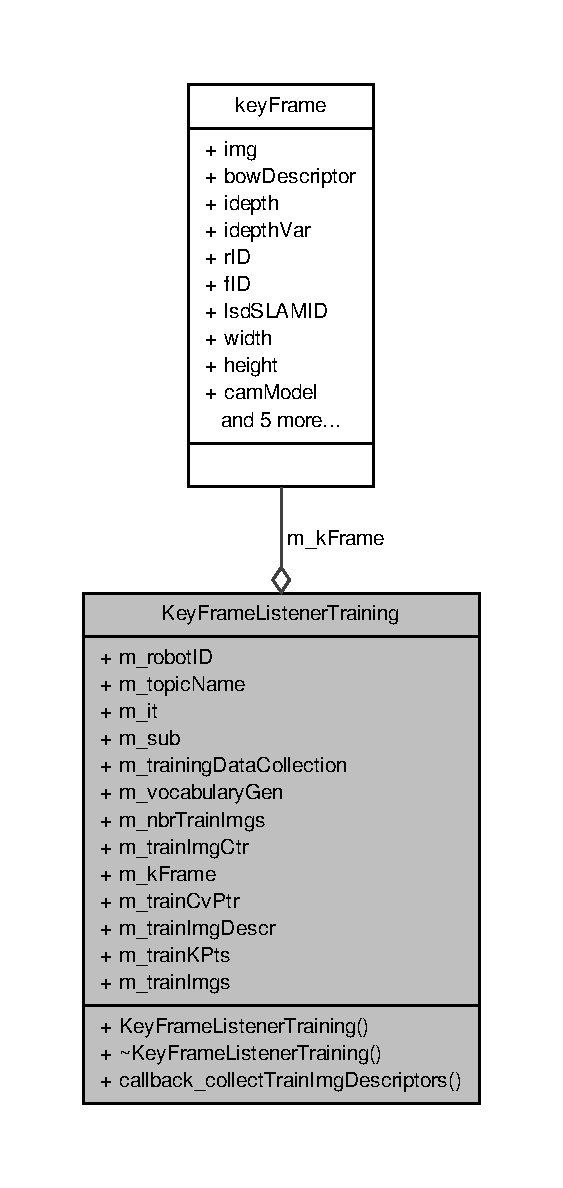
\includegraphics[height=550pt]{classKeyFrameListenerTraining__coll__graph}
\end{center}
\end{figure}
\subsection*{\-Public \-Member \-Functions}
\begin{DoxyCompactItemize}
\item 
\hyperlink{classKeyFrameListenerTraining_a79991f22508bb1680c0913cb6003abb6}{\-Key\-Frame\-Listener\-Training} (int r\-I\-D, int nbr\-Train\-Imgs, string topic\-Name, ros\-::\-Node\-Handle nh, \hyperlink{classCentralStorage}{\-Central\-Storage} $\ast$storage)
\item 
\hyperlink{classKeyFrameListenerTraining_a18c4d5ed913633aafb8ab8173aaf3431}{$\sim$\-Key\-Frame\-Listener\-Training} ()
\begin{DoxyCompactList}\small\item\em destructor \end{DoxyCompactList}\item 
void \hyperlink{classKeyFrameListenerTraining_a437c11f515c20b51d30ef40d637a25ba}{callback\-\_\-collect\-Train\-Img\-Descriptors} (const sensor\-\_\-msgs\-::\-Image\-Const\-Ptr \&msg, \hyperlink{classCentralStorage}{\-Central\-Storage} $\ast$storage)
\begin{DoxyCompactList}\small\item\em \-Member function extracting (\-S\-U\-R\-F) descriptors from training \-Data s.\-t. vocabulary can be created. \end{DoxyCompactList}\end{DoxyCompactItemize}
\subsection*{\-Public \-Attributes}
\begin{DoxyCompactItemize}
\item 
int \hyperlink{classKeyFrameListenerTraining_ac4bc91c462f7cbf1364087c8c7177ee5}{m\-\_\-robot\-I\-D}
\item 
string \hyperlink{classKeyFrameListenerTraining_aa6e0e60a43e678d54a90201c9ec34deb}{m\-\_\-topic\-Name}
\item 
image\-\_\-transport\-::\-Image\-Transport \hyperlink{classKeyFrameListenerTraining_a5063e03ecd884134bbffc0e32dfa71e2}{m\-\_\-it}
\item 
image\-\_\-transport\-::\-Subscriber \hyperlink{classKeyFrameListenerTraining_a3b368cdbbe4bbb92bf47a35d01d55644}{m\-\_\-sub}
\item 
bool \hyperlink{classKeyFrameListenerTraining_a32ea513679de826627bc20c3598bab1b}{m\-\_\-training\-Data\-Collection}
\item 
bool \hyperlink{classKeyFrameListenerTraining_ab9a3dd6c3e61b1ac6271d891bddbd037}{m\-\_\-vocabulary\-Gen}
\item 
int \hyperlink{classKeyFrameListenerTraining_aff6e3d535158a78b464c731d22af308e}{m\-\_\-nbr\-Train\-Imgs}
\begin{DoxyCompactList}\small\item\em nbr of images on which prior should be trained for fabmap = 100 \end{DoxyCompactList}\item 
int \hyperlink{classKeyFrameListenerTraining_a527a1a7e1b02deacba5b417fa61fc367}{m\-\_\-train\-Img\-Ctr}
\begin{DoxyCompactList}\small\item\em counts current nbr of train imgs = 0 \end{DoxyCompactList}\item 
\hyperlink{structkeyFrame}{key\-Frame} \hyperlink{classKeyFrameListenerTraining_af9f9545cdabdc24d58237de03234c10f}{m\-\_\-k\-Frame}
\begin{DoxyCompactList}\small\item\em stores necessary information about one keyframe \end{DoxyCompactList}\item 
cv\-\_\-bridge\-::\-Cv\-Image\-Ptr \hyperlink{classKeyFrameListenerTraining_a6ae5ff8937a42f0d70404b7b8cd572c2}{m\-\_\-train\-Cv\-Ptr}
\begin{DoxyCompactList}\small\item\em save ros sensor img to opencv img \end{DoxyCompactList}\item 
\-Mat \hyperlink{classKeyFrameListenerTraining_a2db812cb925b74093ef76bc16306d9d7}{m\-\_\-train\-Img\-Descr}
\begin{DoxyCompactList}\small\item\em all \-S\-I\-F\-T/\-S\-U\-R\-F descrs. of all train\-Imgs of 1 robot \end{DoxyCompactList}\item 
vector$<$ vector$<$ \-Key\-Point $>$ $>$ \hyperlink{classKeyFrameListenerTraining_a315dd8f41de6cf586c90f600650a908d}{m\-\_\-train\-K\-Pts}
\begin{DoxyCompactList}\small\item\em vec$<$\-K\-Pts$>$\-: all kpts from 1 train\-Img of 1 robot, vec$<$vec$<$\-K\-Pt$>$$>$\-: all \-K\-Pts from all train\-Imgs from 1 robot \end{DoxyCompactList}\item 
vector$<$ \-Mat $>$ \hyperlink{classKeyFrameListenerTraining_a48bd94c8aaabd896a16fd7bb1557e0e7}{m\-\_\-train\-Imgs}
\begin{DoxyCompactList}\small\item\em \-Mat\-: train\-Img, vec$<$\-Mat$>$\-: all train\-Imgs of 1robot. \end{DoxyCompactList}\end{DoxyCompactItemize}


\subsection{\-Detailed \-Description}
\-Class listening to incoming images, each instance of the class listens to one robot -\/$>$ do training. 

\-Definition at line 23 of file \-Key\-Frame\-Listener\-Training.\-h.



\subsection{\-Constructor \& \-Destructor \-Documentation}
\hypertarget{classKeyFrameListenerTraining_a79991f22508bb1680c0913cb6003abb6}{\index{\-Key\-Frame\-Listener\-Training@{\-Key\-Frame\-Listener\-Training}!\-Key\-Frame\-Listener\-Training@{\-Key\-Frame\-Listener\-Training}}
\index{\-Key\-Frame\-Listener\-Training@{\-Key\-Frame\-Listener\-Training}!KeyFrameListenerTraining@{\-Key\-Frame\-Listener\-Training}}
\subsubsection[{\-Key\-Frame\-Listener\-Training}]{\setlength{\rightskip}{0pt plus 5cm}{\bf \-Key\-Frame\-Listener\-Training\-::\-Key\-Frame\-Listener\-Training} (
\begin{DoxyParamCaption}
\item[{int}]{r\-I\-D, }
\item[{int}]{nbr\-Train\-Imgs, }
\item[{string}]{topic\-Name, }
\item[{ros\-::\-Node\-Handle}]{nh, }
\item[{{\bf \-Central\-Storage} $\ast$}]{storage}
\end{DoxyParamCaption}
)}}\label{classKeyFrameListenerTraining_a79991f22508bb1680c0913cb6003abb6}


\-Definition at line 9 of file \-Key\-Frame\-Listener\-Training.\-cpp.


\begin{DoxyCode}
                                                                               
                                                                :
                m_robotID(rID),
                m_nbrTrainImgs(nbrTrainImgs),
                m_it(nh),
                m_trainImgCtr(0)
{
        m_trainingDataCollection = true;
        m_vocabularyGen = false;

        m_sub = m_it.subscribe(topicName, 10, boost::bind(&
      KeyFrameListenerTraining::callback_collectTrainImgDescriptors, this, _1, 
      storage) );
}
\end{DoxyCode}
\hypertarget{classKeyFrameListenerTraining_a18c4d5ed913633aafb8ab8173aaf3431}{\index{\-Key\-Frame\-Listener\-Training@{\-Key\-Frame\-Listener\-Training}!$\sim$\-Key\-Frame\-Listener\-Training@{$\sim$\-Key\-Frame\-Listener\-Training}}
\index{$\sim$\-Key\-Frame\-Listener\-Training@{$\sim$\-Key\-Frame\-Listener\-Training}!KeyFrameListenerTraining@{\-Key\-Frame\-Listener\-Training}}
\subsubsection[{$\sim$\-Key\-Frame\-Listener\-Training}]{\setlength{\rightskip}{0pt plus 5cm}{\bf \-Key\-Frame\-Listener\-Training\-::$\sim$\-Key\-Frame\-Listener\-Training} (
\begin{DoxyParamCaption}
{}
\end{DoxyParamCaption}
)}}\label{classKeyFrameListenerTraining_a18c4d5ed913633aafb8ab8173aaf3431}


destructor 



\-Definition at line 21 of file \-Key\-Frame\-Listener\-Training.\-cpp.


\begin{DoxyCode}
{}
\end{DoxyCode}


\subsection{\-Member \-Function \-Documentation}
\hypertarget{classKeyFrameListenerTraining_a437c11f515c20b51d30ef40d637a25ba}{\index{\-Key\-Frame\-Listener\-Training@{\-Key\-Frame\-Listener\-Training}!callback\-\_\-collect\-Train\-Img\-Descriptors@{callback\-\_\-collect\-Train\-Img\-Descriptors}}
\index{callback\-\_\-collect\-Train\-Img\-Descriptors@{callback\-\_\-collect\-Train\-Img\-Descriptors}!KeyFrameListenerTraining@{\-Key\-Frame\-Listener\-Training}}
\subsubsection[{callback\-\_\-collect\-Train\-Img\-Descriptors}]{\setlength{\rightskip}{0pt plus 5cm}const char {\bf \-Key\-Frame\-Listener\-Training\-::callback\-\_\-collect\-Train\-Img\-Descriptors} (
\begin{DoxyParamCaption}
\item[{const sensor\-\_\-msgs\-::\-Image\-Const\-Ptr \&}]{msg, }
\item[{{\bf \-Central\-Storage} $\ast$}]{storage}
\end{DoxyParamCaption}
)}}\label{classKeyFrameListenerTraining_a437c11f515c20b51d30ef40d637a25ba}


\-Member function extracting (\-S\-U\-R\-F) descriptors from training \-Data s.\-t. vocabulary can be created. 



\-Definition at line 23 of file \-Key\-Frame\-Listener\-Training.\-cpp.


\begin{DoxyCode}
                                                                               
                                                         {

        int skip = 20; // skip (skip) imgs
        try     {
                this->m_trainCvPtr = cv_bridge::toCvCopy(imgMsg, 
      sensor_msgs::image_encodings::BGR8);
        }
        catch (cv_bridge::Exception& e) {
                ROS_ERROR("cv_bridge exception: %s", e.what());
                return;
        }

        
        // ---- START Collect descriptors of all Images (for generating visual
       words later on) ---------------------------------------------------------                
        if(m_trainingDataCollection==true && storage->stopDataCollection == 
      false)
        {

                if((m_trainImgCtr % skip) == 0) // pick every (skip) img of
       video stream
                {
        
                        cout << "Detecting keypoints, computing descriptors of
       training image " << m_trainImgs.size() << endl;

                        // Collect descriptors of all Images
                        Mat trainDescriptorsTmp; // to save descriptors of
       current training Image
                        vector<KeyPoint> trainKPtsTmp; // detected keypoints to
       save keypoints of current training Image
                        (storage->detector)->detect(this->m_trainCvPtr->image,
      trainKPtsTmp);

                        if(trainKPtsTmp.size()>20) {

                                (storage->extractor)->compute(this->m_trainCvPtr
      ->image,trainKPtsTmp,trainDescriptorsTmp);

                                m_trainKPts.push_back(trainKPtsTmp);
                                m_trainImgDescr.push_back(trainDescriptorsTmp);
                                m_trainImgs.push_back(m_trainCvPtr->image);


                                HelperFcts::displayImageKPts("
      currentTrainingImage", m_trainCvPtr->image, trainKPtsTmp);
                                ostringstream convImgName;
                                convImgName << "trainImgs/robot" << m_robotID <
      < "TrainImg" << m_trainImgCtr << ".jpg";
                                string imgName = convImgName.str();
                                HelperFcts::saveImage(m_trainCvPtr->image, 
      imgName);
                        }
                }
                m_trainImgCtr = m_trainImgCtr+1;
        }

        if((m_trainImgs.size() >= m_nbrTrainImgs && m_trainingDataCollection ==
       true) || (storage->stopDataCollection == true && m_trainingDataCollection == 
      true))
        {
                m_trainingDataCollection = false;
                m_vocabularyGen = true;
                storage->stopDataCollection = true;
        }
        // ---- END Collect descriptors of all Images (for generating visual
       words later on) ---------------------------------------------------------
}
\end{DoxyCode}


\subsection{\-Member \-Data \-Documentation}
\hypertarget{classKeyFrameListenerTraining_a5063e03ecd884134bbffc0e32dfa71e2}{\index{\-Key\-Frame\-Listener\-Training@{\-Key\-Frame\-Listener\-Training}!m\-\_\-it@{m\-\_\-it}}
\index{m\-\_\-it@{m\-\_\-it}!KeyFrameListenerTraining@{\-Key\-Frame\-Listener\-Training}}
\subsubsection[{m\-\_\-it}]{\setlength{\rightskip}{0pt plus 5cm}image\-\_\-transport\-::\-Image\-Transport {\bf \-Key\-Frame\-Listener\-Training\-::m\-\_\-it}}}\label{classKeyFrameListenerTraining_a5063e03ecd884134bbffc0e32dfa71e2}


\-Definition at line 30 of file \-Key\-Frame\-Listener\-Training.\-h.

\hypertarget{classKeyFrameListenerTraining_af9f9545cdabdc24d58237de03234c10f}{\index{\-Key\-Frame\-Listener\-Training@{\-Key\-Frame\-Listener\-Training}!m\-\_\-k\-Frame@{m\-\_\-k\-Frame}}
\index{m\-\_\-k\-Frame@{m\-\_\-k\-Frame}!KeyFrameListenerTraining@{\-Key\-Frame\-Listener\-Training}}
\subsubsection[{m\-\_\-k\-Frame}]{\setlength{\rightskip}{0pt plus 5cm}{\bf key\-Frame} {\bf \-Key\-Frame\-Listener\-Training\-::m\-\_\-k\-Frame}}}\label{classKeyFrameListenerTraining_af9f9545cdabdc24d58237de03234c10f}


stores necessary information about one keyframe 



\-Definition at line 39 of file \-Key\-Frame\-Listener\-Training.\-h.

\hypertarget{classKeyFrameListenerTraining_aff6e3d535158a78b464c731d22af308e}{\index{\-Key\-Frame\-Listener\-Training@{\-Key\-Frame\-Listener\-Training}!m\-\_\-nbr\-Train\-Imgs@{m\-\_\-nbr\-Train\-Imgs}}
\index{m\-\_\-nbr\-Train\-Imgs@{m\-\_\-nbr\-Train\-Imgs}!KeyFrameListenerTraining@{\-Key\-Frame\-Listener\-Training}}
\subsubsection[{m\-\_\-nbr\-Train\-Imgs}]{\setlength{\rightskip}{0pt plus 5cm}int {\bf \-Key\-Frame\-Listener\-Training\-::m\-\_\-nbr\-Train\-Imgs}}}\label{classKeyFrameListenerTraining_aff6e3d535158a78b464c731d22af308e}


nbr of images on which prior should be trained for fabmap = 100 



\-Definition at line 36 of file \-Key\-Frame\-Listener\-Training.\-h.

\hypertarget{classKeyFrameListenerTraining_ac4bc91c462f7cbf1364087c8c7177ee5}{\index{\-Key\-Frame\-Listener\-Training@{\-Key\-Frame\-Listener\-Training}!m\-\_\-robot\-I\-D@{m\-\_\-robot\-I\-D}}
\index{m\-\_\-robot\-I\-D@{m\-\_\-robot\-I\-D}!KeyFrameListenerTraining@{\-Key\-Frame\-Listener\-Training}}
\subsubsection[{m\-\_\-robot\-I\-D}]{\setlength{\rightskip}{0pt plus 5cm}int {\bf \-Key\-Frame\-Listener\-Training\-::m\-\_\-robot\-I\-D}}}\label{classKeyFrameListenerTraining_ac4bc91c462f7cbf1364087c8c7177ee5}


\-Definition at line 27 of file \-Key\-Frame\-Listener\-Training.\-h.

\hypertarget{classKeyFrameListenerTraining_a3b368cdbbe4bbb92bf47a35d01d55644}{\index{\-Key\-Frame\-Listener\-Training@{\-Key\-Frame\-Listener\-Training}!m\-\_\-sub@{m\-\_\-sub}}
\index{m\-\_\-sub@{m\-\_\-sub}!KeyFrameListenerTraining@{\-Key\-Frame\-Listener\-Training}}
\subsubsection[{m\-\_\-sub}]{\setlength{\rightskip}{0pt plus 5cm}image\-\_\-transport\-::\-Subscriber {\bf \-Key\-Frame\-Listener\-Training\-::m\-\_\-sub}}}\label{classKeyFrameListenerTraining_a3b368cdbbe4bbb92bf47a35d01d55644}


\-Definition at line 31 of file \-Key\-Frame\-Listener\-Training.\-h.

\hypertarget{classKeyFrameListenerTraining_aa6e0e60a43e678d54a90201c9ec34deb}{\index{\-Key\-Frame\-Listener\-Training@{\-Key\-Frame\-Listener\-Training}!m\-\_\-topic\-Name@{m\-\_\-topic\-Name}}
\index{m\-\_\-topic\-Name@{m\-\_\-topic\-Name}!KeyFrameListenerTraining@{\-Key\-Frame\-Listener\-Training}}
\subsubsection[{m\-\_\-topic\-Name}]{\setlength{\rightskip}{0pt plus 5cm}string {\bf \-Key\-Frame\-Listener\-Training\-::m\-\_\-topic\-Name}}}\label{classKeyFrameListenerTraining_aa6e0e60a43e678d54a90201c9ec34deb}


\-Definition at line 29 of file \-Key\-Frame\-Listener\-Training.\-h.

\hypertarget{classKeyFrameListenerTraining_a6ae5ff8937a42f0d70404b7b8cd572c2}{\index{\-Key\-Frame\-Listener\-Training@{\-Key\-Frame\-Listener\-Training}!m\-\_\-train\-Cv\-Ptr@{m\-\_\-train\-Cv\-Ptr}}
\index{m\-\_\-train\-Cv\-Ptr@{m\-\_\-train\-Cv\-Ptr}!KeyFrameListenerTraining@{\-Key\-Frame\-Listener\-Training}}
\subsubsection[{m\-\_\-train\-Cv\-Ptr}]{\setlength{\rightskip}{0pt plus 5cm}cv\-\_\-bridge\-::\-Cv\-Image\-Ptr {\bf \-Key\-Frame\-Listener\-Training\-::m\-\_\-train\-Cv\-Ptr}}}\label{classKeyFrameListenerTraining_a6ae5ff8937a42f0d70404b7b8cd572c2}


save ros sensor img to opencv img 



\-Definition at line 40 of file \-Key\-Frame\-Listener\-Training.\-h.

\hypertarget{classKeyFrameListenerTraining_a527a1a7e1b02deacba5b417fa61fc367}{\index{\-Key\-Frame\-Listener\-Training@{\-Key\-Frame\-Listener\-Training}!m\-\_\-train\-Img\-Ctr@{m\-\_\-train\-Img\-Ctr}}
\index{m\-\_\-train\-Img\-Ctr@{m\-\_\-train\-Img\-Ctr}!KeyFrameListenerTraining@{\-Key\-Frame\-Listener\-Training}}
\subsubsection[{m\-\_\-train\-Img\-Ctr}]{\setlength{\rightskip}{0pt plus 5cm}int {\bf \-Key\-Frame\-Listener\-Training\-::m\-\_\-train\-Img\-Ctr}}}\label{classKeyFrameListenerTraining_a527a1a7e1b02deacba5b417fa61fc367}


counts current nbr of train imgs = 0 



\-Definition at line 37 of file \-Key\-Frame\-Listener\-Training.\-h.

\hypertarget{classKeyFrameListenerTraining_a2db812cb925b74093ef76bc16306d9d7}{\index{\-Key\-Frame\-Listener\-Training@{\-Key\-Frame\-Listener\-Training}!m\-\_\-train\-Img\-Descr@{m\-\_\-train\-Img\-Descr}}
\index{m\-\_\-train\-Img\-Descr@{m\-\_\-train\-Img\-Descr}!KeyFrameListenerTraining@{\-Key\-Frame\-Listener\-Training}}
\subsubsection[{m\-\_\-train\-Img\-Descr}]{\setlength{\rightskip}{0pt plus 5cm}\-Mat {\bf \-Key\-Frame\-Listener\-Training\-::m\-\_\-train\-Img\-Descr}}}\label{classKeyFrameListenerTraining_a2db812cb925b74093ef76bc16306d9d7}


all \-S\-I\-F\-T/\-S\-U\-R\-F descrs. of all train\-Imgs of 1 robot 



\-Definition at line 42 of file \-Key\-Frame\-Listener\-Training.\-h.

\hypertarget{classKeyFrameListenerTraining_a48bd94c8aaabd896a16fd7bb1557e0e7}{\index{\-Key\-Frame\-Listener\-Training@{\-Key\-Frame\-Listener\-Training}!m\-\_\-train\-Imgs@{m\-\_\-train\-Imgs}}
\index{m\-\_\-train\-Imgs@{m\-\_\-train\-Imgs}!KeyFrameListenerTraining@{\-Key\-Frame\-Listener\-Training}}
\subsubsection[{m\-\_\-train\-Imgs}]{\setlength{\rightskip}{0pt plus 5cm}vector$<$\-Mat$>$ {\bf \-Key\-Frame\-Listener\-Training\-::m\-\_\-train\-Imgs}}}\label{classKeyFrameListenerTraining_a48bd94c8aaabd896a16fd7bb1557e0e7}


\-Mat\-: train\-Img, vec$<$\-Mat$>$\-: all train\-Imgs of 1robot. 



\-Definition at line 44 of file \-Key\-Frame\-Listener\-Training.\-h.

\hypertarget{classKeyFrameListenerTraining_a32ea513679de826627bc20c3598bab1b}{\index{\-Key\-Frame\-Listener\-Training@{\-Key\-Frame\-Listener\-Training}!m\-\_\-training\-Data\-Collection@{m\-\_\-training\-Data\-Collection}}
\index{m\-\_\-training\-Data\-Collection@{m\-\_\-training\-Data\-Collection}!KeyFrameListenerTraining@{\-Key\-Frame\-Listener\-Training}}
\subsubsection[{m\-\_\-training\-Data\-Collection}]{\setlength{\rightskip}{0pt plus 5cm}bool {\bf \-Key\-Frame\-Listener\-Training\-::m\-\_\-training\-Data\-Collection}}}\label{classKeyFrameListenerTraining_a32ea513679de826627bc20c3598bab1b}


\-Definition at line 33 of file \-Key\-Frame\-Listener\-Training.\-h.

\hypertarget{classKeyFrameListenerTraining_a315dd8f41de6cf586c90f600650a908d}{\index{\-Key\-Frame\-Listener\-Training@{\-Key\-Frame\-Listener\-Training}!m\-\_\-train\-K\-Pts@{m\-\_\-train\-K\-Pts}}
\index{m\-\_\-train\-K\-Pts@{m\-\_\-train\-K\-Pts}!KeyFrameListenerTraining@{\-Key\-Frame\-Listener\-Training}}
\subsubsection[{m\-\_\-train\-K\-Pts}]{\setlength{\rightskip}{0pt plus 5cm}vector$<$vector$<$\-Key\-Point$>$ $>$ {\bf \-Key\-Frame\-Listener\-Training\-::m\-\_\-train\-K\-Pts}}}\label{classKeyFrameListenerTraining_a315dd8f41de6cf586c90f600650a908d}


vec$<$\-K\-Pts$>$\-: all kpts from 1 train\-Img of 1 robot, vec$<$vec$<$\-K\-Pt$>$$>$\-: all \-K\-Pts from all train\-Imgs from 1 robot 



\-Definition at line 43 of file \-Key\-Frame\-Listener\-Training.\-h.

\hypertarget{classKeyFrameListenerTraining_ab9a3dd6c3e61b1ac6271d891bddbd037}{\index{\-Key\-Frame\-Listener\-Training@{\-Key\-Frame\-Listener\-Training}!m\-\_\-vocabulary\-Gen@{m\-\_\-vocabulary\-Gen}}
\index{m\-\_\-vocabulary\-Gen@{m\-\_\-vocabulary\-Gen}!KeyFrameListenerTraining@{\-Key\-Frame\-Listener\-Training}}
\subsubsection[{m\-\_\-vocabulary\-Gen}]{\setlength{\rightskip}{0pt plus 5cm}bool {\bf \-Key\-Frame\-Listener\-Training\-::m\-\_\-vocabulary\-Gen}}}\label{classKeyFrameListenerTraining_ab9a3dd6c3e61b1ac6271d891bddbd037}


\-Definition at line 34 of file \-Key\-Frame\-Listener\-Training.\-h.



\-The documentation for this class was generated from the following files\-:\begin{DoxyCompactItemize}
\item 
\hyperlink{KeyFrameListenerTraining_8h}{\-Key\-Frame\-Listener\-Training.\-h}\item 
\hyperlink{KeyFrameListenerTraining_8cpp}{\-Key\-Frame\-Listener\-Training.\-cpp}\end{DoxyCompactItemize}

\hypertarget{classNode}{\section{\-Node \-Class \-Reference}
\label{classNode}\index{\-Node@{\-Node}}
}


{\ttfamily \#include $<$\-Pose\-Graph.\-h$>$}



\-Collaboration diagram for \-Node\-:\nopagebreak
\begin{figure}[H]
\begin{center}
\leavevmode
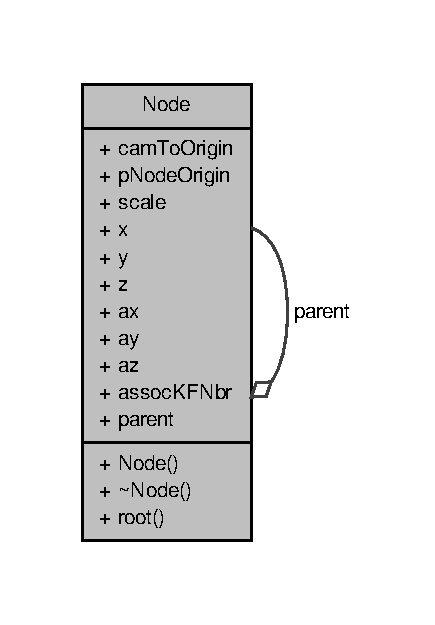
\includegraphics[width=209pt]{classNode__coll__graph}
\end{center}
\end{figure}
\subsection*{\-Public \-Member \-Functions}
\begin{DoxyCompactItemize}
\item 
\hyperlink{classNode_ad7a34779cad45d997bfd6d3d8043c75f}{\-Node} ()
\item 
\hyperlink{classNode_aa0840c3cb5c7159be6d992adecd2097c}{$\sim$\-Node} ()
\item 
\hyperlink{classNode}{\-Node} $\ast$ \hyperlink{classNode_a9e417fbf8c05319b464890592e384e42}{root} ()
\end{DoxyCompactItemize}
\subsection*{\-Public \-Attributes}
\begin{DoxyCompactItemize}
\item 
float \hyperlink{classNode_a090a2028b74112aba3eb2126d99028aa}{cam\-To\-Origin} \mbox{[}7\mbox{]}
\item 
\-Eigen\-::\-Matrix4f \hyperlink{classNode_a440bd555088974667fa25d81788e5d7b}{p\-Node\-Origin}
\item 
float \hyperlink{classNode_a60234c70b368f633adc297393a429269}{scale}
\item 
float \hyperlink{classNode_a3a6b88b82c51d21305656d01e3c53039}{x}
\item 
float \hyperlink{classNode_a0658e9aa67d95daa5da3cca23b13f6de}{y}
\item 
float \hyperlink{classNode_ab0676d1ca50996c875aad2e6773d758c}{z}
\item 
float \hyperlink{classNode_a8b0379c6d5f819d6f840d2e623c20f5d}{ax}
\item 
float \hyperlink{classNode_a1815f050e4c4d0864255d33f05e992ea}{ay}
\item 
float \hyperlink{classNode_a55bba6ef3a51e6ab04e4e1612343335a}{az}
\item 
int \hyperlink{classNode_a7969f3edc8046afe7b7601d78e52c3c3}{assoc\-K\-F\-Nbr}
\item 
\hyperlink{classNode}{\-Node} $\ast$ \hyperlink{classNode_ad8184598cdea70e4bbdfd76f2b0f9e85}{parent}
\end{DoxyCompactItemize}


\subsection{\-Detailed \-Description}


\-Definition at line 12 of file \-Pose\-Graph.\-h.



\subsection{\-Constructor \& \-Destructor \-Documentation}
\hypertarget{classNode_ad7a34779cad45d997bfd6d3d8043c75f}{\index{\-Node@{\-Node}!\-Node@{\-Node}}
\index{\-Node@{\-Node}!Node@{\-Node}}
\subsubsection[{\-Node}]{\setlength{\rightskip}{0pt plus 5cm}{\bf \-Node\-::\-Node} (
\begin{DoxyParamCaption}
{}
\end{DoxyParamCaption}
)}}\label{classNode_ad7a34779cad45d997bfd6d3d8043c75f}


\-Definition at line 5 of file \-Pose\-Graph.\-cpp.


\begin{DoxyCode}
           : x(0.0), y(0.0), z(0.0),
                ax(0.0), ay(0.0), az(0.0),
                assocKFNbr(0) {
        parent = NULL;
}
\end{DoxyCode}
\hypertarget{classNode_aa0840c3cb5c7159be6d992adecd2097c}{\index{\-Node@{\-Node}!$\sim$\-Node@{$\sim$\-Node}}
\index{$\sim$\-Node@{$\sim$\-Node}!Node@{\-Node}}
\subsubsection[{$\sim$\-Node}]{\setlength{\rightskip}{0pt plus 5cm}{\bf \-Node\-::$\sim$\-Node} (
\begin{DoxyParamCaption}
{}
\end{DoxyParamCaption}
)}}\label{classNode_aa0840c3cb5c7159be6d992adecd2097c}


\-Definition at line 11 of file \-Pose\-Graph.\-cpp.


\begin{DoxyCode}
{}
\end{DoxyCode}


\subsection{\-Member \-Function \-Documentation}
\hypertarget{classNode_a9e417fbf8c05319b464890592e384e42}{\index{\-Node@{\-Node}!root@{root}}
\index{root@{root}!Node@{\-Node}}
\subsubsection[{root}]{\setlength{\rightskip}{0pt plus 5cm}{\bf \-Node} $\ast$ {\bf \-Node\-::root} (
\begin{DoxyParamCaption}
{}
\end{DoxyParamCaption}
)}}\label{classNode_a9e417fbf8c05319b464890592e384e42}


\-Definition at line 13 of file \-Pose\-Graph.\-cpp.


\begin{DoxyCode}
                  {
        Node *cur = this;
        while(cur!=cur->parent) {
                cur=cur->parent;
        }
        this->parent = cur; //do path compression
        return cur;
}
\end{DoxyCode}


\subsection{\-Member \-Data \-Documentation}
\hypertarget{classNode_a7969f3edc8046afe7b7601d78e52c3c3}{\index{\-Node@{\-Node}!assoc\-K\-F\-Nbr@{assoc\-K\-F\-Nbr}}
\index{assoc\-K\-F\-Nbr@{assoc\-K\-F\-Nbr}!Node@{\-Node}}
\subsubsection[{assoc\-K\-F\-Nbr}]{\setlength{\rightskip}{0pt plus 5cm}int {\bf \-Node\-::assoc\-K\-F\-Nbr}}}\label{classNode_a7969f3edc8046afe7b7601d78e52c3c3}


\-Definition at line 22 of file \-Pose\-Graph.\-h.

\hypertarget{classNode_a8b0379c6d5f819d6f840d2e623c20f5d}{\index{\-Node@{\-Node}!ax@{ax}}
\index{ax@{ax}!Node@{\-Node}}
\subsubsection[{ax}]{\setlength{\rightskip}{0pt plus 5cm}float {\bf \-Node\-::ax}}}\label{classNode_a8b0379c6d5f819d6f840d2e623c20f5d}


\-Definition at line 20 of file \-Pose\-Graph.\-h.

\hypertarget{classNode_a1815f050e4c4d0864255d33f05e992ea}{\index{\-Node@{\-Node}!ay@{ay}}
\index{ay@{ay}!Node@{\-Node}}
\subsubsection[{ay}]{\setlength{\rightskip}{0pt plus 5cm}float {\bf \-Node\-::ay}}}\label{classNode_a1815f050e4c4d0864255d33f05e992ea}


\-Definition at line 20 of file \-Pose\-Graph.\-h.

\hypertarget{classNode_a55bba6ef3a51e6ab04e4e1612343335a}{\index{\-Node@{\-Node}!az@{az}}
\index{az@{az}!Node@{\-Node}}
\subsubsection[{az}]{\setlength{\rightskip}{0pt plus 5cm}float {\bf \-Node\-::az}}}\label{classNode_a55bba6ef3a51e6ab04e4e1612343335a}


\-Definition at line 20 of file \-Pose\-Graph.\-h.

\hypertarget{classNode_a090a2028b74112aba3eb2126d99028aa}{\index{\-Node@{\-Node}!cam\-To\-Origin@{cam\-To\-Origin}}
\index{cam\-To\-Origin@{cam\-To\-Origin}!Node@{\-Node}}
\subsubsection[{cam\-To\-Origin}]{\setlength{\rightskip}{0pt plus 5cm}float {\bf \-Node\-::cam\-To\-Origin}\mbox{[}7\mbox{]}}}\label{classNode_a090a2028b74112aba3eb2126d99028aa}


\-Definition at line 16 of file \-Pose\-Graph.\-h.

\hypertarget{classNode_ad8184598cdea70e4bbdfd76f2b0f9e85}{\index{\-Node@{\-Node}!parent@{parent}}
\index{parent@{parent}!Node@{\-Node}}
\subsubsection[{parent}]{\setlength{\rightskip}{0pt plus 5cm}{\bf \-Node}$\ast$ {\bf \-Node\-::parent}}}\label{classNode_ad8184598cdea70e4bbdfd76f2b0f9e85}


\-Definition at line 24 of file \-Pose\-Graph.\-h.

\hypertarget{classNode_a440bd555088974667fa25d81788e5d7b}{\index{\-Node@{\-Node}!p\-Node\-Origin@{p\-Node\-Origin}}
\index{p\-Node\-Origin@{p\-Node\-Origin}!Node@{\-Node}}
\subsubsection[{p\-Node\-Origin}]{\setlength{\rightskip}{0pt plus 5cm}\-Eigen\-::\-Matrix4f {\bf \-Node\-::p\-Node\-Origin}}}\label{classNode_a440bd555088974667fa25d81788e5d7b}


\-Definition at line 17 of file \-Pose\-Graph.\-h.

\hypertarget{classNode_a60234c70b368f633adc297393a429269}{\index{\-Node@{\-Node}!scale@{scale}}
\index{scale@{scale}!Node@{\-Node}}
\subsubsection[{scale}]{\setlength{\rightskip}{0pt plus 5cm}float {\bf \-Node\-::scale}}}\label{classNode_a60234c70b368f633adc297393a429269}


\-Definition at line 18 of file \-Pose\-Graph.\-h.

\hypertarget{classNode_a3a6b88b82c51d21305656d01e3c53039}{\index{\-Node@{\-Node}!x@{x}}
\index{x@{x}!Node@{\-Node}}
\subsubsection[{x}]{\setlength{\rightskip}{0pt plus 5cm}float {\bf \-Node\-::x}}}\label{classNode_a3a6b88b82c51d21305656d01e3c53039}


\-Definition at line 19 of file \-Pose\-Graph.\-h.

\hypertarget{classNode_a0658e9aa67d95daa5da3cca23b13f6de}{\index{\-Node@{\-Node}!y@{y}}
\index{y@{y}!Node@{\-Node}}
\subsubsection[{y}]{\setlength{\rightskip}{0pt plus 5cm}float {\bf \-Node\-::y}}}\label{classNode_a0658e9aa67d95daa5da3cca23b13f6de}


\-Definition at line 19 of file \-Pose\-Graph.\-h.

\hypertarget{classNode_ab0676d1ca50996c875aad2e6773d758c}{\index{\-Node@{\-Node}!z@{z}}
\index{z@{z}!Node@{\-Node}}
\subsubsection[{z}]{\setlength{\rightskip}{0pt plus 5cm}float {\bf \-Node\-::z}}}\label{classNode_ab0676d1ca50996c875aad2e6773d758c}


\-Definition at line 19 of file \-Pose\-Graph.\-h.



\-The documentation for this class was generated from the following files\-:\begin{DoxyCompactItemize}
\item 
\hyperlink{PoseGraph_8h}{\-Pose\-Graph.\-h}\item 
\hyperlink{PoseGraph_8cpp}{\-Pose\-Graph.\-cpp}\end{DoxyCompactItemize}

\hypertarget{classPoseGraph}{\section{\-Pose\-Graph \-Class \-Reference}
\label{classPoseGraph}\index{\-Pose\-Graph@{\-Pose\-Graph}}
}


{\ttfamily \#include $<$\-Pose\-Graph.\-h$>$}

\subsection*{\-Public \-Member \-Functions}
\begin{DoxyCompactItemize}
\item 
\hyperlink{classPoseGraph_a3b9befc3778d6b8c6abd264d81e72611}{\-Pose\-Graph} ()
\item 
\hyperlink{classPoseGraph_a68fd3df8bf8d4d89d7d51fd318edefea}{$\sim$\-Pose\-Graph} ()
\item 
void \hyperlink{classPoseGraph_a983f26181ccdcacdfa2e399ff6ce76bd}{clear} ()
\end{DoxyCompactItemize}
\subsection*{\-Public \-Attributes}
\begin{DoxyCompactItemize}
\item 
std\-::map$<$ int, \hyperlink{classNode}{\-Node} $>$ \hyperlink{classPoseGraph_aeebc9858b540e6f182c4fb0d491fc073}{nodes}
\item 
std\-::map$<$ int, \hyperlink{classEdge}{\-Edge} $>$ \hyperlink{classPoseGraph_aee9648a8057b16239650ef1d610d43af}{edges}
\end{DoxyCompactItemize}


\subsection{\-Detailed \-Description}


\-Definition at line 50 of file \-Pose\-Graph.\-h.



\subsection{\-Constructor \& \-Destructor \-Documentation}
\hypertarget{classPoseGraph_a3b9befc3778d6b8c6abd264d81e72611}{\index{\-Pose\-Graph@{\-Pose\-Graph}!\-Pose\-Graph@{\-Pose\-Graph}}
\index{\-Pose\-Graph@{\-Pose\-Graph}!PoseGraph@{\-Pose\-Graph}}
\subsubsection[{\-Pose\-Graph}]{\setlength{\rightskip}{0pt plus 5cm}{\bf \-Pose\-Graph\-::\-Pose\-Graph} (
\begin{DoxyParamCaption}
{}
\end{DoxyParamCaption}
)}}\label{classPoseGraph_a3b9befc3778d6b8c6abd264d81e72611}


\-Definition at line 44 of file \-Pose\-Graph.\-cpp.


\begin{DoxyCode}
: nodes(), edges() {}
\end{DoxyCode}
\hypertarget{classPoseGraph_a68fd3df8bf8d4d89d7d51fd318edefea}{\index{\-Pose\-Graph@{\-Pose\-Graph}!$\sim$\-Pose\-Graph@{$\sim$\-Pose\-Graph}}
\index{$\sim$\-Pose\-Graph@{$\sim$\-Pose\-Graph}!PoseGraph@{\-Pose\-Graph}}
\subsubsection[{$\sim$\-Pose\-Graph}]{\setlength{\rightskip}{0pt plus 5cm}{\bf \-Pose\-Graph\-::$\sim$\-Pose\-Graph} (
\begin{DoxyParamCaption}
{}
\end{DoxyParamCaption}
)}}\label{classPoseGraph_a68fd3df8bf8d4d89d7d51fd318edefea}


\-Definition at line 46 of file \-Pose\-Graph.\-cpp.


\begin{DoxyCode}
{}
\end{DoxyCode}


\subsection{\-Member \-Function \-Documentation}
\hypertarget{classPoseGraph_a983f26181ccdcacdfa2e399ff6ce76bd}{\index{\-Pose\-Graph@{\-Pose\-Graph}!clear@{clear}}
\index{clear@{clear}!PoseGraph@{\-Pose\-Graph}}
\subsubsection[{clear}]{\setlength{\rightskip}{0pt plus 5cm}void {\bf \-Pose\-Graph\-::clear} (
\begin{DoxyParamCaption}
{}
\end{DoxyParamCaption}
)}}\label{classPoseGraph_a983f26181ccdcacdfa2e399ff6ce76bd}


\-Definition at line 48 of file \-Pose\-Graph.\-cpp.


\begin{DoxyCode}
                      {
        nodes.clear();
        edges.clear();
}
\end{DoxyCode}


\subsection{\-Member \-Data \-Documentation}
\hypertarget{classPoseGraph_aee9648a8057b16239650ef1d610d43af}{\index{\-Pose\-Graph@{\-Pose\-Graph}!edges@{edges}}
\index{edges@{edges}!PoseGraph@{\-Pose\-Graph}}
\subsubsection[{edges}]{\setlength{\rightskip}{0pt plus 5cm}std\-::map$<$int, {\bf \-Edge}$>$ {\bf \-Pose\-Graph\-::edges}}}\label{classPoseGraph_aee9648a8057b16239650ef1d610d43af}


\-Definition at line 53 of file \-Pose\-Graph.\-h.

\hypertarget{classPoseGraph_aeebc9858b540e6f182c4fb0d491fc073}{\index{\-Pose\-Graph@{\-Pose\-Graph}!nodes@{nodes}}
\index{nodes@{nodes}!PoseGraph@{\-Pose\-Graph}}
\subsubsection[{nodes}]{\setlength{\rightskip}{0pt plus 5cm}std\-::map$<$int, {\bf \-Node}$>$ {\bf \-Pose\-Graph\-::nodes}}}\label{classPoseGraph_aeebc9858b540e6f182c4fb0d491fc073}


\-Definition at line 52 of file \-Pose\-Graph.\-h.



\-The documentation for this class was generated from the following files\-:\begin{DoxyCompactItemize}
\item 
\hyperlink{PoseGraph_8h}{\-Pose\-Graph.\-h}\item 
\hyperlink{PoseGraph_8cpp}{\-Pose\-Graph.\-cpp}\end{DoxyCompactItemize}

\hypertarget{classSyncListener}{\section{\-Sync\-Listener \-Class \-Reference}
\label{classSyncListener}\index{\-Sync\-Listener@{\-Sync\-Listener}}
}


\-Class listening to incoming \-Msgs and synchronizes them, each instance of the class listens to one robot.  




{\ttfamily \#include $<$\-Sync\-Listener.\-h$>$}



\-Collaboration diagram for \-Sync\-Listener\-:\nopagebreak
\begin{figure}[H]
\begin{center}
\leavevmode
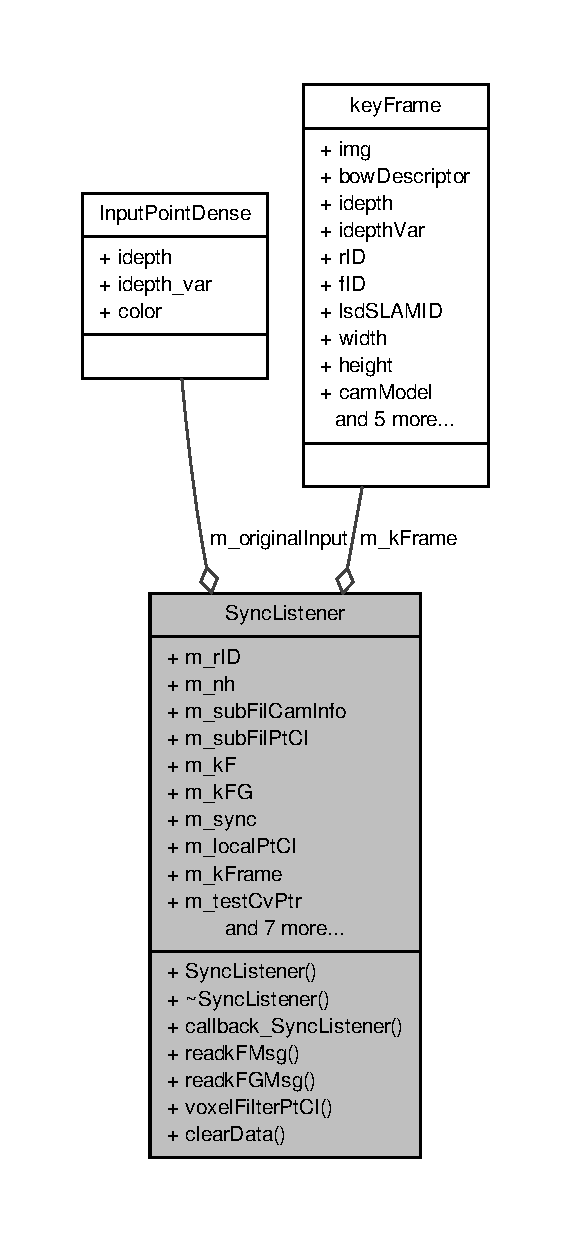
\includegraphics[height=550pt]{classSyncListener__coll__graph}
\end{center}
\end{figure}
\subsection*{\-Public \-Types}
\begin{DoxyCompactItemize}
\item 
typedef \*
sync\-\_\-policies\-::\-Approximate\-Time\*
$<$ \-Camera\-Info, \-Point\-Cloud2, \*
cc\-\_\-fabmap\-::keyframe\-Msg\-Stamped, \*
cc\-\_\-fabmap\-::keyframe\-Graph\-Msg\-Stamped $>$ \hyperlink{classSyncListener_aff51e417f521f074342bc0344856d01e}{\-My\-Sync\-Policy}
\end{DoxyCompactItemize}
\subsection*{\-Public \-Member \-Functions}
\begin{DoxyCompactItemize}
\item 
\hyperlink{classSyncListener_ae69658445cf77c60360e14748cce3129}{\-Sync\-Listener} (int r\-I\-D, string cam\-Info\-Topic\-Name, string pt\-Cl\-Topic\-Name, string k\-F\-Topic\-Name, string k\-F\-G\-Topic\-Name, ros\-::\-Node\-Handle nh, \hyperlink{classCentralStorage}{\-Central\-Storage} $\ast$storage)
\begin{DoxyCompactList}\small\item\em \-Constructor initializing member variables. \end{DoxyCompactList}\item 
\hyperlink{classSyncListener_a3e0b75c3cca66f812fc3eac4f9c4d36c}{$\sim$\-Sync\-Listener} ()
\begin{DoxyCompactList}\small\item\em destructor \end{DoxyCompactList}\item 
void \hyperlink{classSyncListener_a7eb4b7e88109cb8a2e352bd7454d6af6}{callback\-\_\-\-Sync\-Listener} (const \-Camera\-Info\-Const\-Ptr \&cam\-Info\-Msg, const \-Point\-Cloud2\-Const\-Ptr \&pt\-Cl\-Msg, const cc\-\_\-fabmap\-::keyframe\-Msg\-Stamped\-::\-Const\-Ptr \&k\-F\-Msg, const cc\-\_\-fabmap\-::keyframe\-Graph\-Msg\-Stamped\-::\-Const\-Ptr \&k\-F\-G\-Msg, \hyperlink{classCentralStorage}{\-Central\-Storage} $\ast$storage)
\begin{DoxyCompactList}\small\item\em \-Member function listening to incoming \-Msgs. \end{DoxyCompactList}\item 
void \hyperlink{classSyncListener_a2343c140657ed44918b69d4ccfc0f2fc}{readk\-F\-Msg} (const cc\-\_\-fabmap\-::keyframe\-Msg\-Stamped\-::\-Const\-Ptr \&k\-F\-Msg)
\item 
void \hyperlink{classSyncListener_a15eba5d8398bbee26167f14498d39a44}{readk\-F\-G\-Msg} (const cc\-\_\-fabmap\-::keyframe\-Graph\-Msg\-Stamped\-::\-Const\-Ptr \&k\-F\-G\-Msg, \hyperlink{classCentralStorage}{\-Central\-Storage} $\ast$storage)
\item 
void \hyperlink{classSyncListener_a5b6fc157cbff88f505051895be194580}{voxel\-Filter\-Pt\-Cl} (\hyperlink{classCentralStorage}{\-Central\-Storage} $\ast$storage)
\item 
void \hyperlink{classSyncListener_afb1bc8df5e84e851cd63e875222cdaa1}{clear\-Data} ()
\end{DoxyCompactItemize}
\subsection*{\-Public \-Attributes}
\begin{DoxyCompactItemize}
\item 
int \hyperlink{classSyncListener_a8a56de9b7444cfe79845217863f50ac4}{m\-\_\-r\-I\-D}
\item 
ros\-::\-Node\-Handle \hyperlink{classSyncListener_a11af18cee056cd6558e11246c86d746c}{m\-\_\-nh}
\item 
message\-\_\-filters\-::\-Subscriber\*
$<$ \-Camera\-Info $>$ \hyperlink{classSyncListener_a8a2f8f014180ef641c4f23edc60f7f65}{m\-\_\-sub\-Fil\-Cam\-Info}
\item 
message\-\_\-filters\-::\-Subscriber\*
$<$ \-Point\-Cloud2 $>$ \hyperlink{classSyncListener_ac23b28241b0e85d1247f3bb116bdfeaf}{m\-\_\-sub\-Fil\-Pt\-Cl}
\item 
message\-\_\-filters\-::\-Subscriber\*
$<$ cc\-\_\-fabmap\-::keyframe\-Msg\-Stamped $>$ \hyperlink{classSyncListener_a283e6f9b1bb60cfe3fdf43787faddbb0}{m\-\_\-k\-F}
\item 
message\-\_\-filters\-::\-Subscriber\*
$<$ cc\-\_\-fabmap\-::keyframe\-Graph\-Msg\-Stamped $>$ \hyperlink{classSyncListener_a80a7b642798ea3441475ab9c57567345}{m\-\_\-k\-F\-G}
\item 
\-Synchronizer$<$ \hyperlink{classSyncListener_aff51e417f521f074342bc0344856d01e}{\-My\-Sync\-Policy} $>$ \hyperlink{classSyncListener_a2f352324b76a40e4e7b6cb560f527b2c}{m\-\_\-sync}
\item 
pcl\-::\-Point\-Cloud$<$ pcl\-::\-Point\-X\-Y\-Z $>$\*
\-::\-Ptr \hyperlink{classSyncListener_adf1510f0bffe657a07972b53265462a7}{m\-\_\-local\-Pt\-Cl}
\item 
\hyperlink{structkeyFrame}{key\-Frame} \hyperlink{classSyncListener_a4d09eece5d98418ba9f0d5e2b78739db}{m\-\_\-k\-Frame}
\begin{DoxyCompactList}\small\item\em stores necessary information about one keyframe \end{DoxyCompactList}\item 
cv\-\_\-bridge\-::\-Cv\-Image\-Ptr \hyperlink{classSyncListener_a86ba5fc553e1a656b7643c09e865aebb}{m\-\_\-test\-Cv\-Ptr}
\begin{DoxyCompactList}\small\item\em save ros sensor img to opencv img \end{DoxyCompactList}\item 
vector$<$ \-Key\-Point $>$ \hyperlink{classSyncListener_a6ebc46a18ad7a9acb1d00a7373959572}{m\-\_\-test\-K\-Pts}
\begin{DoxyCompactList}\small\item\em vec$<$\-K\-Pts$>$\-: all kpts from 1 test\-Img of 1 robot \end{DoxyCompactList}\item 
geometry\-\_\-msgs\-::\-Pose\-Stamped \hyperlink{classSyncListener_a17fb054f6825f7b44eeab7467938ac81}{m\-\_\-local\-Pose}
\item 
\-Eigen\-::\-Translation$<$ float, 3 $>$ \hyperlink{classSyncListener_a1dc58db5a86d88a47fdad97920a31d4c}{m\-\_\-sim3\-Local\-Pose\-Transl}
\item 
\-Eigen\-::\-Quaternion$<$ float $>$ \hyperlink{classSyncListener_ab56ff407af05f490da548a5e7150a726}{m\-\_\-sim3\-Local\-Pose\-Quat}
\item 
float \hyperlink{classSyncListener_aaf3e2d41bade5563773335eb7dcea484}{m\-\_\-sim3\-Local\-Pose\-Scale}
\item 
\hyperlink{structInputPointDense}{\-Input\-Point\-Dense} $\ast$ \hyperlink{classSyncListener_a143bf4683b219a962032a3b711820850}{m\-\_\-original\-Input}
\item 
std\-::map$<$ int, \hyperlink{classNode}{\-Node} $>$ \hyperlink{classSyncListener_a8f72710aa41f9f4b48c23ac1d5f37e23}{nodes}
\item 
std\-::map$<$ int, \hyperlink{classEdge}{\-Edge} $>$ \hyperlink{classSyncListener_a681672fb8569101a794d8c7d8a8c1448}{edges}
\end{DoxyCompactItemize}


\subsection{\-Detailed \-Description}
\-Class listening to incoming \-Msgs and synchronizes them, each instance of the class listens to one robot. 

\-Definition at line 64 of file \-Sync\-Listener.\-h.



\subsection{\-Member \-Typedef \-Documentation}
\hypertarget{classSyncListener_aff51e417f521f074342bc0344856d01e}{\index{\-Sync\-Listener@{\-Sync\-Listener}!\-My\-Sync\-Policy@{\-My\-Sync\-Policy}}
\index{\-My\-Sync\-Policy@{\-My\-Sync\-Policy}!SyncListener@{\-Sync\-Listener}}
\subsubsection[{\-My\-Sync\-Policy}]{\setlength{\rightskip}{0pt plus 5cm}typedef sync\-\_\-policies\-::\-Approximate\-Time$<$ \-Camera\-Info, \-Point\-Cloud2, cc\-\_\-fabmap\-::keyframe\-Msg\-Stamped, cc\-\_\-fabmap\-::keyframe\-Graph\-Msg\-Stamped$>$ {\bf \-Sync\-Listener\-::\-My\-Sync\-Policy}}}\label{classSyncListener_aff51e417f521f074342bc0344856d01e}


\-Definition at line 80 of file \-Sync\-Listener.\-h.



\subsection{\-Constructor \& \-Destructor \-Documentation}
\hypertarget{classSyncListener_ae69658445cf77c60360e14748cce3129}{\index{\-Sync\-Listener@{\-Sync\-Listener}!\-Sync\-Listener@{\-Sync\-Listener}}
\index{\-Sync\-Listener@{\-Sync\-Listener}!SyncListener@{\-Sync\-Listener}}
\subsubsection[{\-Sync\-Listener}]{\setlength{\rightskip}{0pt plus 5cm}const char {\bf \-Sync\-Listener\-::\-Sync\-Listener} (
\begin{DoxyParamCaption}
\item[{int}]{r\-I\-D, }
\item[{string}]{cam\-Info\-Topic\-Name, }
\item[{string}]{pt\-Cl\-Topic\-Name, }
\item[{string}]{k\-F\-Topic\-Name, }
\item[{string}]{k\-F\-G\-Topic\-Name, }
\item[{ros\-::\-Node\-Handle}]{nh, }
\item[{{\bf \-Central\-Storage} $\ast$}]{storage}
\end{DoxyParamCaption}
)}}\label{classSyncListener_ae69658445cf77c60360e14748cce3129}


\-Constructor initializing member variables. 



\-Definition at line 23 of file \-Sync\-Listener.\-cpp.


\begin{DoxyCode}
                                                           :
                m_rID(rID),
                m_nh(nh),
                m_subFilCamInfo(nh,camInfoTopicName,100),
                m_subFilPtCl(nh,ptClTopicName,100),
                m_kF(nh,kFTopicName,100),
                m_kFG(nh,kFGTopicName,100),
                m_sync(MySyncPolicy(100), m_subFilCamInfo, m_subFilPtCl, m_kF, 
      m_kFG),
                m_localPtCl(new pcl::PointCloud<pcl::PointXYZ>)
{
        m_sync.registerCallback(boost::bind(&SyncListener::callback_SyncListener
      , this, _1, _2, _3, _4, storage));
        m_originalInput = NULL;
        m_kFrame.img =  cv::Mat(480,640,CV_8UC3, Scalar(0,0,255));
}
\end{DoxyCode}
\hypertarget{classSyncListener_a3e0b75c3cca66f812fc3eac4f9c4d36c}{\index{\-Sync\-Listener@{\-Sync\-Listener}!$\sim$\-Sync\-Listener@{$\sim$\-Sync\-Listener}}
\index{$\sim$\-Sync\-Listener@{$\sim$\-Sync\-Listener}!SyncListener@{\-Sync\-Listener}}
\subsubsection[{$\sim$\-Sync\-Listener}]{\setlength{\rightskip}{0pt plus 5cm}{\bf \-Sync\-Listener\-::$\sim$\-Sync\-Listener} (
\begin{DoxyParamCaption}
{}
\end{DoxyParamCaption}
)}}\label{classSyncListener_a3e0b75c3cca66f812fc3eac4f9c4d36c}


destructor 



\-Definition at line 43 of file \-Sync\-Listener.\-cpp.


\begin{DoxyCode}
{}
\end{DoxyCode}


\subsection{\-Member \-Function \-Documentation}
\hypertarget{classSyncListener_a7eb4b7e88109cb8a2e352bd7454d6af6}{\index{\-Sync\-Listener@{\-Sync\-Listener}!callback\-\_\-\-Sync\-Listener@{callback\-\_\-\-Sync\-Listener}}
\index{callback\-\_\-\-Sync\-Listener@{callback\-\_\-\-Sync\-Listener}!SyncListener@{\-Sync\-Listener}}
\subsubsection[{callback\-\_\-\-Sync\-Listener}]{\setlength{\rightskip}{0pt plus 5cm}const char {\bf \-Sync\-Listener\-::callback\-\_\-\-Sync\-Listener} (
\begin{DoxyParamCaption}
\item[{const \-Camera\-Info\-Const\-Ptr \&}]{cam\-Info\-Msg, }
\item[{const \-Point\-Cloud2\-Const\-Ptr \&}]{pt\-Cl\-Msg, }
\item[{const cc\-\_\-fabmap\-::keyframe\-Msg\-Stamped\-::\-Const\-Ptr \&}]{k\-F\-Msg, }
\item[{const cc\-\_\-fabmap\-::keyframe\-Graph\-Msg\-Stamped\-::\-Const\-Ptr \&}]{k\-F\-G\-Msg, }
\item[{{\bf \-Central\-Storage} $\ast$}]{storage}
\end{DoxyParamCaption}
)}}\label{classSyncListener_a7eb4b7e88109cb8a2e352bd7454d6af6}


\-Member function listening to incoming \-Msgs. 



\-Definition at line 46 of file \-Sync\-Listener.\-cpp.


\begin{DoxyCode}
                                         {

        // Cam Info Listener
        // cam mat stays constant --> no need to process anything
        storage->camModel.fromCameraInfo(camInfoMsg);

        // PtCl Listener
        pcl::fromROSMsg( *ptClMsg, *this->m_localPtCl );
        // Downsample PtCl
        //this->voxelFilterPtCl(storage);

        // kFMsg Listener
        // kFMsg contains the coordinate Transformation from Camera Frame of
       the corresponding robot to the initial robot frame
        // By taking the inverse, the pose of the Frame is revealed
        this->readkFMsg(kFMsg);
        this->m_kFrame.rID = this->m_rID;

        //kFGraphMsg Listener
        this->readkFGMsg(kFGMsg, storage);

        (storage->detector)->detect(this->m_kFrame.img,this->m_kFrame.KPts);

        // this->m_kFrame.camToRobot = tRobotCam = pCamRobot
        // m_localPose = pCamRobot =
        HelperFcts::trafoFloat7ToQuatTranslScale(this->m_kFrame.camToRobot, 
      this->m_sim3LocalPoseQuat, this->m_sim3LocalPoseTransl, this->m_sim3LocalPoseScale)
      ;
        // get Pose from coordinate transformation (message contains a
       coordinate transformation!!!)
        //HelperFcts::invQuatTranslScale(this->m_sim3LocalPoseQuat,
       this->m_sim3LocalPoseQuat, this->m_sim3LocalPoseTransl, this->m_sim3LocalPoseTransl,
       this->m_sim3LocalPoseScale, this->m_sim3LocalPoseScale);
        HelperFcts::eigenQuatTranslPoseToROSPose(this->m_sim3LocalPoseQuat, 
      this->m_sim3LocalPoseTransl, this->m_localPose);


        // JUST FOR CHECKING IF SOPHUS EQUAL OWN IMPLEMENTATION
//      memcpy(m_sim3LocalPose.data(), simTrafoMsg->sim3f.data(),
       7*sizeof(float));
//      cout << endl << endl<< endl;
//      cout << "Sophus: " << this->m_sim3LocalPose.translation() << endl;
//      cout << this->m_sim3LocalPose.quaternion().w() << " " <<
       this->m_sim3LocalPose.quaternion().x() << " " << this->m_sim3LocalPose.quaternion().y() << " "
       << this->m_sim3LocalPose.quaternion().z() << endl;
//      cout << "scale: " << this->m_sim3LocalPose.scale() << endl;
//      cout <<
       this->m_sim3LocalPose.quaternion().w()/this->m_sim3LocalPose.scale() << " " <<
       this->m_sim3LocalPose.quaternion().x()/this->m_sim3LocalPose.scale() << " " << this->m_sim3LocalPose.quaternion().y() << " " <<
       this->m_sim3LocalPose.quaternion().z()/this->m_sim3LocalPose.scale() << endl << endl;
//      cout << "Eigen: " << this->m_localPose.pose.position.x << " " <<
       this->m_localPose.pose.position.y << " " << this->m_localPose.pose.position.z << endl;
//      cout << this->m_localPose.pose.orientation.w << " " <<
       this->m_localPose.pose.orientation.x << " " << this->m_localPose.pose.orientation.y << " " <<
       this->m_localPose.pose.orientation.z << endl;
//      cout << "scale: " << this->m_sim3LocalPoseScale << endl;
//      cout << endl << endl<< endl;

}
\end{DoxyCode}
\hypertarget{classSyncListener_afb1bc8df5e84e851cd63e875222cdaa1}{\index{\-Sync\-Listener@{\-Sync\-Listener}!clear\-Data@{clear\-Data}}
\index{clear\-Data@{clear\-Data}!SyncListener@{\-Sync\-Listener}}
\subsubsection[{clear\-Data}]{\setlength{\rightskip}{0pt plus 5cm}void {\bf \-Sync\-Listener\-::clear\-Data} (
\begin{DoxyParamCaption}
{}
\end{DoxyParamCaption}
)}}\label{classSyncListener_afb1bc8df5e84e851cd63e875222cdaa1}


\-Definition at line 180 of file \-Sync\-Listener.\-cpp.


\begin{DoxyCode}
                             {

        for( int i=0; i<7; ++i ) {
                this->m_kFrame.camToRobot[i] = 0.0;
                if(i==3) {
                        this->m_kFrame.camToRobot[i] = 1.0;
                }
        }
        this->m_kFrame.cx = 0;
        this->m_kFrame.cy = 0;
        this->m_kFrame.fx = 0;
        this->m_kFrame.fy = 0;
        this->m_kFrame.height = 0;
        this->m_kFrame.width = 0;
        this->m_kFrame.idepth.release();
        this->m_kFrame.idepthVar.release();
        this->m_kFrame.img.release();
        this->m_kFrame.KPts.clear();
        this->m_kFrame.bowDescriptor.release();
        this->m_kFrame.fID = 0;
        this->m_kFrame.rID = 0;
        this->m_kFrame.lsdSLAMID = 0;

        this->m_testKPts.clear();
        this->m_localPtCl->clear();
        this->m_sim3LocalPoseTransl.x() = this->m_sim3LocalPoseTransl.y() = 
      this->m_sim3LocalPoseTransl.z() = 0.0;
        this->m_sim3LocalPoseQuat.setIdentity();
        this->m_sim3LocalPoseScale = 0.0;

        this->m_originalInput = NULL;

        this->nodes.clear();
        this->edges.clear();
}
\end{DoxyCode}
\hypertarget{classSyncListener_a15eba5d8398bbee26167f14498d39a44}{\index{\-Sync\-Listener@{\-Sync\-Listener}!readk\-F\-G\-Msg@{readk\-F\-G\-Msg}}
\index{readk\-F\-G\-Msg@{readk\-F\-G\-Msg}!SyncListener@{\-Sync\-Listener}}
\subsubsection[{readk\-F\-G\-Msg}]{\setlength{\rightskip}{0pt plus 5cm}void {\bf \-Sync\-Listener\-::readk\-F\-G\-Msg} (
\begin{DoxyParamCaption}
\item[{const cc\-\_\-fabmap\-::keyframe\-Graph\-Msg\-Stamped\-::\-Const\-Ptr \&}]{k\-F\-G\-Msg, }
\item[{{\bf \-Central\-Storage} $\ast$}]{storage}
\end{DoxyParamCaption}
)}}\label{classSyncListener_a15eba5d8398bbee26167f14498d39a44}


\-Definition at line 145 of file \-Sync\-Listener.\-cpp.


\begin{DoxyCode}
                                                                               
                                     {
        // Get information for graph
        GraphFramePose* graphPoses = (GraphFramePose*)kFGMsg->frameData.data();
        int numGraphPoses = kFGMsg->numFrames;

        //cout << "numFrames" << kFGMsg->numFrames << endl;
        //cout << "numConstraints" << kFGMsg->numConstraints << endl;

        for( int nbrNode=0 ; nbrNode<numGraphPoses ; nbrNode++ ) {
                int fID = -1000;
                lsdSLAMIDToFID(storage, graphPoses[nbrNode].id, fID);
                //cout << "graphPoses[nbrNode].id: " << graphPoses[nbrNode].id
       << " fID: " << fID << endl;

                if(fID == -1000) {
                //      printf("ERROR: graph update contains pose for frame %d,
       but I dont have a frame %d!\n", graphPoses[nbrNode].id,
       graphPoses[nbrNode].id);
                }
                else {
                        for(int i=0; i<7; ++i) {
                                nodes[fID].camToOrigin[i] = graphPoses[nbrNode]
      .camToWorld[i];
                        }
                }
        }
}
\end{DoxyCode}
\hypertarget{classSyncListener_a2343c140657ed44918b69d4ccfc0f2fc}{\index{\-Sync\-Listener@{\-Sync\-Listener}!readk\-F\-Msg@{readk\-F\-Msg}}
\index{readk\-F\-Msg@{readk\-F\-Msg}!SyncListener@{\-Sync\-Listener}}
\subsubsection[{readk\-F\-Msg}]{\setlength{\rightskip}{0pt plus 5cm}void {\bf \-Sync\-Listener\-::readk\-F\-Msg} (
\begin{DoxyParamCaption}
\item[{const cc\-\_\-fabmap\-::keyframe\-Msg\-Stamped\-::\-Const\-Ptr \&}]{k\-F\-Msg}
\end{DoxyParamCaption}
)}}\label{classSyncListener_a2343c140657ed44918b69d4ccfc0f2fc}


\-Definition at line 94 of file \-Sync\-Listener.\-cpp.


\begin{DoxyCode}
                                                                             {

        for(int i=0 ; i<7 ; ++i) {
                this->m_kFrame.camToRobot[i] = kFMsg->camToWorld[i];
        }

        this->m_kFrame.width = kFMsg->width;
        this->m_kFrame.height = kFMsg->height;
        this->m_kFrame.fx = kFMsg->fx;
        this->m_kFrame.fy = kFMsg->fy;
        this->m_kFrame.cx = kFMsg->cx;
        this->m_kFrame.cy = kFMsg->cy;
        this->m_kFrame.lsdSLAMID = kFMsg->id;

        if(this->m_originalInput != 0) {
                delete[] this->m_originalInput;
        }

        this->m_originalInput=0;

        if(kFMsg->pointcloud.size() != this->m_kFrame.width*this->m_kFrame.
      height*sizeof(InputPointDense)) {
                if(kFMsg->pointcloud.size() != 0)
                {
                        cout << "WARNING" << endl;
                        //printf("WARNING: PC with points, but number of points
       not right! (is %zu, should be %u*%dx%d=%u)\n",
                                        //kFMsg->pointcloud.size(),
       sizeof(InputPointDense), this->m_kFrame.width, this->m_kFrame.height,
       this->m_kFrame.width*this->m_kFrame.height*sizeof(InputPointDense));
                }
        }
        else {
                this->m_originalInput = new InputPointDense[this->m_kFrame.width
      * this->m_kFrame.height];
                memcpy( this->m_originalInput, kFMsg->pointcloud.data(), this->
      m_kFrame.width* this->m_kFrame.height*sizeof(InputPointDense));
        }

        this->m_kFrame.img = cv::Mat(480,640,CV_8UC3, Scalar(0,0,255));
        this->m_kFrame.idepth = cv::Mat(480,640,CV_32FC1, Scalar(0,0,255));
        this->m_kFrame.idepthVar = cv::Mat(480,640,CV_32FC1, Scalar(0,0,255));
        for( int y=0 ; y<this->m_kFrame.height-1 ; y++ ) {
                for( int x=0 ; x<this->m_kFrame.width-1 ; x++) {
                        cv::Vec3b bgr;

                        bgr[0] = this->m_originalInput[x+y*this->m_kFrame.width
      ].color[0];
                        bgr[1] = this->m_originalInput[x+y*this->m_kFrame.width
      ].color[1];
                        bgr[2] = this->m_originalInput[x+y*this->m_kFrame.width
      ].color[2];

                        this->m_kFrame.img.at< Vec3b >( cv::Point(x,y) ) = bgr;
                        this->m_kFrame.idepth.at< float >(y,x) = this->
      m_originalInput->idepth;
                        this->m_kFrame.idepthVar.at< float >(y,x) = this->
      m_originalInput->idepth_var;
                }
        }
}
\end{DoxyCode}
\hypertarget{classSyncListener_a5b6fc157cbff88f505051895be194580}{\index{\-Sync\-Listener@{\-Sync\-Listener}!voxel\-Filter\-Pt\-Cl@{voxel\-Filter\-Pt\-Cl}}
\index{voxel\-Filter\-Pt\-Cl@{voxel\-Filter\-Pt\-Cl}!SyncListener@{\-Sync\-Listener}}
\subsubsection[{voxel\-Filter\-Pt\-Cl}]{\setlength{\rightskip}{0pt plus 5cm}void {\bf \-Sync\-Listener\-::voxel\-Filter\-Pt\-Cl} (
\begin{DoxyParamCaption}
\item[{{\bf \-Central\-Storage} $\ast$}]{storage}
\end{DoxyParamCaption}
)}}\label{classSyncListener_a5b6fc157cbff88f505051895be194580}


\-Definition at line 169 of file \-Sync\-Listener.\-cpp.


\begin{DoxyCode}
                                                          {

        // Create the filtering object
        pcl::VoxelGrid< pcl::PointXYZ > sor;

        sor.setInputCloud ( (this->m_localPtCl) );
        sor.setLeafSize (0.001f, 0.001f, 0.001f);
        sor.filter ( *(this->m_localPtCl) );

}
\end{DoxyCode}


\subsection{\-Member \-Data \-Documentation}
\hypertarget{classSyncListener_a681672fb8569101a794d8c7d8a8c1448}{\index{\-Sync\-Listener@{\-Sync\-Listener}!edges@{edges}}
\index{edges@{edges}!SyncListener@{\-Sync\-Listener}}
\subsubsection[{edges}]{\setlength{\rightskip}{0pt plus 5cm}std\-::map$<$int,{\bf \-Edge}$>$ {\bf \-Sync\-Listener\-::edges}}}\label{classSyncListener_a681672fb8569101a794d8c7d8a8c1448}


\-Definition at line 103 of file \-Sync\-Listener.\-h.

\hypertarget{classSyncListener_a283e6f9b1bb60cfe3fdf43787faddbb0}{\index{\-Sync\-Listener@{\-Sync\-Listener}!m\-\_\-k\-F@{m\-\_\-k\-F}}
\index{m\-\_\-k\-F@{m\-\_\-k\-F}!SyncListener@{\-Sync\-Listener}}
\subsubsection[{m\-\_\-k\-F}]{\setlength{\rightskip}{0pt plus 5cm}message\-\_\-filters\-::\-Subscriber$<$cc\-\_\-fabmap\-::keyframe\-Msg\-Stamped$>$ {\bf \-Sync\-Listener\-::m\-\_\-k\-F}}}\label{classSyncListener_a283e6f9b1bb60cfe3fdf43787faddbb0}


\-Definition at line 74 of file \-Sync\-Listener.\-h.

\hypertarget{classSyncListener_a80a7b642798ea3441475ab9c57567345}{\index{\-Sync\-Listener@{\-Sync\-Listener}!m\-\_\-k\-F\-G@{m\-\_\-k\-F\-G}}
\index{m\-\_\-k\-F\-G@{m\-\_\-k\-F\-G}!SyncListener@{\-Sync\-Listener}}
\subsubsection[{m\-\_\-k\-F\-G}]{\setlength{\rightskip}{0pt plus 5cm}message\-\_\-filters\-::\-Subscriber$<$cc\-\_\-fabmap\-::keyframe\-Graph\-Msg\-Stamped$>$ {\bf \-Sync\-Listener\-::m\-\_\-k\-F\-G}}}\label{classSyncListener_a80a7b642798ea3441475ab9c57567345}


\-Definition at line 75 of file \-Sync\-Listener.\-h.

\hypertarget{classSyncListener_a4d09eece5d98418ba9f0d5e2b78739db}{\index{\-Sync\-Listener@{\-Sync\-Listener}!m\-\_\-k\-Frame@{m\-\_\-k\-Frame}}
\index{m\-\_\-k\-Frame@{m\-\_\-k\-Frame}!SyncListener@{\-Sync\-Listener}}
\subsubsection[{m\-\_\-k\-Frame}]{\setlength{\rightskip}{0pt plus 5cm}{\bf key\-Frame} {\bf \-Sync\-Listener\-::m\-\_\-k\-Frame}}}\label{classSyncListener_a4d09eece5d98418ba9f0d5e2b78739db}


stores necessary information about one keyframe 



\-Definition at line 89 of file \-Sync\-Listener.\-h.

\hypertarget{classSyncListener_a17fb054f6825f7b44eeab7467938ac81}{\index{\-Sync\-Listener@{\-Sync\-Listener}!m\-\_\-local\-Pose@{m\-\_\-local\-Pose}}
\index{m\-\_\-local\-Pose@{m\-\_\-local\-Pose}!SyncListener@{\-Sync\-Listener}}
\subsubsection[{m\-\_\-local\-Pose}]{\setlength{\rightskip}{0pt plus 5cm}geometry\-\_\-msgs\-::\-Pose\-Stamped {\bf \-Sync\-Listener\-::m\-\_\-local\-Pose}}}\label{classSyncListener_a17fb054f6825f7b44eeab7467938ac81}


\-Definition at line 93 of file \-Sync\-Listener.\-h.

\hypertarget{classSyncListener_adf1510f0bffe657a07972b53265462a7}{\index{\-Sync\-Listener@{\-Sync\-Listener}!m\-\_\-local\-Pt\-Cl@{m\-\_\-local\-Pt\-Cl}}
\index{m\-\_\-local\-Pt\-Cl@{m\-\_\-local\-Pt\-Cl}!SyncListener@{\-Sync\-Listener}}
\subsubsection[{m\-\_\-local\-Pt\-Cl}]{\setlength{\rightskip}{0pt plus 5cm}pcl\-::\-Point\-Cloud$<$pcl\-::\-Point\-X\-Y\-Z$>$\-::\-Ptr {\bf \-Sync\-Listener\-::m\-\_\-local\-Pt\-Cl}}}\label{classSyncListener_adf1510f0bffe657a07972b53265462a7}


\-Definition at line 86 of file \-Sync\-Listener.\-h.

\hypertarget{classSyncListener_a11af18cee056cd6558e11246c86d746c}{\index{\-Sync\-Listener@{\-Sync\-Listener}!m\-\_\-nh@{m\-\_\-nh}}
\index{m\-\_\-nh@{m\-\_\-nh}!SyncListener@{\-Sync\-Listener}}
\subsubsection[{m\-\_\-nh}]{\setlength{\rightskip}{0pt plus 5cm}ros\-::\-Node\-Handle {\bf \-Sync\-Listener\-::m\-\_\-nh}}}\label{classSyncListener_a11af18cee056cd6558e11246c86d746c}


\-Definition at line 70 of file \-Sync\-Listener.\-h.

\hypertarget{classSyncListener_a143bf4683b219a962032a3b711820850}{\index{\-Sync\-Listener@{\-Sync\-Listener}!m\-\_\-original\-Input@{m\-\_\-original\-Input}}
\index{m\-\_\-original\-Input@{m\-\_\-original\-Input}!SyncListener@{\-Sync\-Listener}}
\subsubsection[{m\-\_\-original\-Input}]{\setlength{\rightskip}{0pt plus 5cm}{\bf \-Input\-Point\-Dense}$\ast$ {\bf \-Sync\-Listener\-::m\-\_\-original\-Input}}}\label{classSyncListener_a143bf4683b219a962032a3b711820850}


\-Definition at line 99 of file \-Sync\-Listener.\-h.

\hypertarget{classSyncListener_a8a56de9b7444cfe79845217863f50ac4}{\index{\-Sync\-Listener@{\-Sync\-Listener}!m\-\_\-r\-I\-D@{m\-\_\-r\-I\-D}}
\index{m\-\_\-r\-I\-D@{m\-\_\-r\-I\-D}!SyncListener@{\-Sync\-Listener}}
\subsubsection[{m\-\_\-r\-I\-D}]{\setlength{\rightskip}{0pt plus 5cm}int {\bf \-Sync\-Listener\-::m\-\_\-r\-I\-D}}}\label{classSyncListener_a8a56de9b7444cfe79845217863f50ac4}


\-Definition at line 68 of file \-Sync\-Listener.\-h.

\hypertarget{classSyncListener_ab56ff407af05f490da548a5e7150a726}{\index{\-Sync\-Listener@{\-Sync\-Listener}!m\-\_\-sim3\-Local\-Pose\-Quat@{m\-\_\-sim3\-Local\-Pose\-Quat}}
\index{m\-\_\-sim3\-Local\-Pose\-Quat@{m\-\_\-sim3\-Local\-Pose\-Quat}!SyncListener@{\-Sync\-Listener}}
\subsubsection[{m\-\_\-sim3\-Local\-Pose\-Quat}]{\setlength{\rightskip}{0pt plus 5cm}\-Eigen\-::\-Quaternion$<$float$>$ {\bf \-Sync\-Listener\-::m\-\_\-sim3\-Local\-Pose\-Quat}}}\label{classSyncListener_ab56ff407af05f490da548a5e7150a726}


\-Definition at line 96 of file \-Sync\-Listener.\-h.

\hypertarget{classSyncListener_aaf3e2d41bade5563773335eb7dcea484}{\index{\-Sync\-Listener@{\-Sync\-Listener}!m\-\_\-sim3\-Local\-Pose\-Scale@{m\-\_\-sim3\-Local\-Pose\-Scale}}
\index{m\-\_\-sim3\-Local\-Pose\-Scale@{m\-\_\-sim3\-Local\-Pose\-Scale}!SyncListener@{\-Sync\-Listener}}
\subsubsection[{m\-\_\-sim3\-Local\-Pose\-Scale}]{\setlength{\rightskip}{0pt plus 5cm}float {\bf \-Sync\-Listener\-::m\-\_\-sim3\-Local\-Pose\-Scale}}}\label{classSyncListener_aaf3e2d41bade5563773335eb7dcea484}


\-Definition at line 97 of file \-Sync\-Listener.\-h.

\hypertarget{classSyncListener_a1dc58db5a86d88a47fdad97920a31d4c}{\index{\-Sync\-Listener@{\-Sync\-Listener}!m\-\_\-sim3\-Local\-Pose\-Transl@{m\-\_\-sim3\-Local\-Pose\-Transl}}
\index{m\-\_\-sim3\-Local\-Pose\-Transl@{m\-\_\-sim3\-Local\-Pose\-Transl}!SyncListener@{\-Sync\-Listener}}
\subsubsection[{m\-\_\-sim3\-Local\-Pose\-Transl}]{\setlength{\rightskip}{0pt plus 5cm}\-Eigen\-::\-Translation$<$float,3$>$ {\bf \-Sync\-Listener\-::m\-\_\-sim3\-Local\-Pose\-Transl}}}\label{classSyncListener_a1dc58db5a86d88a47fdad97920a31d4c}


\-Definition at line 95 of file \-Sync\-Listener.\-h.

\hypertarget{classSyncListener_a8a2f8f014180ef641c4f23edc60f7f65}{\index{\-Sync\-Listener@{\-Sync\-Listener}!m\-\_\-sub\-Fil\-Cam\-Info@{m\-\_\-sub\-Fil\-Cam\-Info}}
\index{m\-\_\-sub\-Fil\-Cam\-Info@{m\-\_\-sub\-Fil\-Cam\-Info}!SyncListener@{\-Sync\-Listener}}
\subsubsection[{m\-\_\-sub\-Fil\-Cam\-Info}]{\setlength{\rightskip}{0pt plus 5cm}message\-\_\-filters\-::\-Subscriber$<$\-Camera\-Info$>$ {\bf \-Sync\-Listener\-::m\-\_\-sub\-Fil\-Cam\-Info}}}\label{classSyncListener_a8a2f8f014180ef641c4f23edc60f7f65}


\-Definition at line 72 of file \-Sync\-Listener.\-h.

\hypertarget{classSyncListener_ac23b28241b0e85d1247f3bb116bdfeaf}{\index{\-Sync\-Listener@{\-Sync\-Listener}!m\-\_\-sub\-Fil\-Pt\-Cl@{m\-\_\-sub\-Fil\-Pt\-Cl}}
\index{m\-\_\-sub\-Fil\-Pt\-Cl@{m\-\_\-sub\-Fil\-Pt\-Cl}!SyncListener@{\-Sync\-Listener}}
\subsubsection[{m\-\_\-sub\-Fil\-Pt\-Cl}]{\setlength{\rightskip}{0pt plus 5cm}message\-\_\-filters\-::\-Subscriber$<$\-Point\-Cloud2$>$ {\bf \-Sync\-Listener\-::m\-\_\-sub\-Fil\-Pt\-Cl}}}\label{classSyncListener_ac23b28241b0e85d1247f3bb116bdfeaf}


\-Definition at line 73 of file \-Sync\-Listener.\-h.

\hypertarget{classSyncListener_a2f352324b76a40e4e7b6cb560f527b2c}{\index{\-Sync\-Listener@{\-Sync\-Listener}!m\-\_\-sync@{m\-\_\-sync}}
\index{m\-\_\-sync@{m\-\_\-sync}!SyncListener@{\-Sync\-Listener}}
\subsubsection[{m\-\_\-sync}]{\setlength{\rightskip}{0pt plus 5cm}\-Synchronizer$<${\bf \-My\-Sync\-Policy}$>$ {\bf \-Sync\-Listener\-::m\-\_\-sync}}}\label{classSyncListener_a2f352324b76a40e4e7b6cb560f527b2c}


\-Definition at line 81 of file \-Sync\-Listener.\-h.

\hypertarget{classSyncListener_a86ba5fc553e1a656b7643c09e865aebb}{\index{\-Sync\-Listener@{\-Sync\-Listener}!m\-\_\-test\-Cv\-Ptr@{m\-\_\-test\-Cv\-Ptr}}
\index{m\-\_\-test\-Cv\-Ptr@{m\-\_\-test\-Cv\-Ptr}!SyncListener@{\-Sync\-Listener}}
\subsubsection[{m\-\_\-test\-Cv\-Ptr}]{\setlength{\rightskip}{0pt plus 5cm}cv\-\_\-bridge\-::\-Cv\-Image\-Ptr {\bf \-Sync\-Listener\-::m\-\_\-test\-Cv\-Ptr}}}\label{classSyncListener_a86ba5fc553e1a656b7643c09e865aebb}


save ros sensor img to opencv img 



\-Definition at line 90 of file \-Sync\-Listener.\-h.

\hypertarget{classSyncListener_a6ebc46a18ad7a9acb1d00a7373959572}{\index{\-Sync\-Listener@{\-Sync\-Listener}!m\-\_\-test\-K\-Pts@{m\-\_\-test\-K\-Pts}}
\index{m\-\_\-test\-K\-Pts@{m\-\_\-test\-K\-Pts}!SyncListener@{\-Sync\-Listener}}
\subsubsection[{m\-\_\-test\-K\-Pts}]{\setlength{\rightskip}{0pt plus 5cm}vector$<$\-Key\-Point$>$ {\bf \-Sync\-Listener\-::m\-\_\-test\-K\-Pts}}}\label{classSyncListener_a6ebc46a18ad7a9acb1d00a7373959572}


vec$<$\-K\-Pts$>$\-: all kpts from 1 test\-Img of 1 robot 



\-Definition at line 91 of file \-Sync\-Listener.\-h.

\hypertarget{classSyncListener_a8f72710aa41f9f4b48c23ac1d5f37e23}{\index{\-Sync\-Listener@{\-Sync\-Listener}!nodes@{nodes}}
\index{nodes@{nodes}!SyncListener@{\-Sync\-Listener}}
\subsubsection[{nodes}]{\setlength{\rightskip}{0pt plus 5cm}std\-::map$<$int,{\bf \-Node}$>$ {\bf \-Sync\-Listener\-::nodes}}}\label{classSyncListener_a8f72710aa41f9f4b48c23ac1d5f37e23}


\-Definition at line 102 of file \-Sync\-Listener.\-h.



\-The documentation for this class was generated from the following files\-:\begin{DoxyCompactItemize}
\item 
\hyperlink{SyncListener_8h}{\-Sync\-Listener.\-h}\item 
\hyperlink{SyncListener_8cpp}{\-Sync\-Listener.\-cpp}\end{DoxyCompactItemize}

\chapter{\-File \-Documentation}
\hypertarget{cc__fabmap__node_8cpp}{\section{cc\-\_\-fabmap\-\_\-node.\-cpp \-File \-Reference}
\label{cc__fabmap__node_8cpp}\index{cc\-\_\-fabmap\-\_\-node.\-cpp@{cc\-\_\-fabmap\-\_\-node.\-cpp}}
}
{\ttfamily \#include $<$ros/ros.\-h$>$}\*
{\ttfamily \#include $<$sensor\-\_\-msgs/image\-\_\-encodings.\-h$>$}\*
{\ttfamily \#include $<$message\-\_\-filters/subscriber.\-h$>$}\*
{\ttfamily \#include $<$sensor\-\_\-msgs/\-Image.\-h$>$}\*
{\ttfamily \#include $<$message\-\_\-filters/time\-\_\-synchronizer.\-h$>$}\*
{\ttfamily \#include $<$tf/transform\-\_\-broadcaster.\-h$>$}\*
{\ttfamily \#include $<$image\-\_\-transport/image\-\_\-transport.\-h$>$}\*
{\ttfamily \#include $<$cv\-\_\-bridge/cv\-\_\-bridge.\-h$>$}\*
{\ttfamily \#include $<$opencv2/highgui/highgui.\-hpp$>$}\*
{\ttfamily \#include $<$opencv2/imgproc/imgproc.\-hpp$>$}\*
{\ttfamily \#include $<$opencv2/opencv.\-hpp$>$}\*
{\ttfamily \#include \char`\"{}opencv2/nonfree/nonfree.\-hpp\char`\"{}}\*
{\ttfamily \#include \char`\"{}\-Key\-Frame\-Listener\-Training.\-h\char`\"{}}\*
{\ttfamily \#include \char`\"{}\-Sync\-Listener.\-h\char`\"{}}\*
\-Include dependency graph for cc\-\_\-fabmap\-\_\-node.\-cpp\-:\nopagebreak
\begin{figure}[H]
\begin{center}
\leavevmode

\includegraphics[width=350pt]{cc__fabmap__node_8cpp__incl}
\end{center}
\end{figure}
\subsection*{\-Functions}
\begin{DoxyCompactItemize}
\item 
void \hyperlink{cc__fabmap__node_8cpp_a99cb8485ba55364caae90a9d3d8d6609}{helper\-Disp\-Output} (\hyperlink{classCentralStorage}{\-Central\-Storage} $\ast$storage, bool save\-Match\-Matrix=false, string match\-Matrix\-Name\-Img=\char`\"{}\char`\"{}, string match\-Matrix\-Name\-File=\char`\"{}\char`\"{})
\item 
void \hyperlink{cc__fabmap__node_8cpp_a959fee195cd952ecb7f06befa08f4024}{helper\-Get\-Test\-Data} (\hyperlink{classCentralStorage}{\-Central\-Storage} $\ast$storage)
\item 
void \hyperlink{cc__fabmap__node_8cpp_a9665aef254686f428f555d32c1b30fa8}{helper\-Publish\-Assembled\-Global\-Pt\-Cl} (\hyperlink{classCentralStorage}{\-Central\-Storage} $\ast$storage, ros\-::\-Publisher \&pub, int skip\-First\-N)
\item 
void \hyperlink{cc__fabmap__node_8cpp_a085df1b3fc0cf52d21284c92297e891c}{helper\-Publish\-Assembled\-Local\-Pt\-Cl} (\hyperlink{classCentralStorage}{\-Central\-Storage} $\ast$storage, int r\-I\-D, ros\-::\-Publisher \&pub, int skip\-First\-N)
\item 
void \hyperlink{cc__fabmap__node_8cpp_aa9b6e90f43cc74d5b9e6a0d4d4304eef}{helper\-Publish\-Pt\-Cl} (pcl\-::\-Point\-Cloud$<$ pcl\-::\-Point\-X\-Y\-Z $>$ pt\-Cl, ros\-::\-Publisher \&pub)
\item 
void \hyperlink{cc__fabmap__node_8cpp_a2a2548ab36e98be49fd91e373ee89684}{helper\-Read\-Train\-Data} (\hyperlink{classCentralStorage}{\-Central\-Storage} $\ast$storage)
\item 
void \hyperlink{cc__fabmap__node_8cpp_a8254506cb42ab9e85d3123dbbea7ce49}{helper\-Save\-Test\-Imgs} (\hyperlink{classCentralStorage}{\-Central\-Storage} $\ast$storage, \hyperlink{classSyncListener}{\-Sync\-Listener} \&listener\-\_\-r1, \hyperlink{classSyncListener}{\-Sync\-Listener} \&listener\-\_\-r2)
\item 
void \hyperlink{cc__fabmap__node_8cpp_a060e73dd74d1e5d07b42755cd9ffb1e2}{helper\-Save\-Train\-Data} (\hyperlink{classCentralStorage}{\-Central\-Storage} $\ast$storage)
\item 
void \hyperlink{cc__fabmap__node_8cpp_af41fb2ed487a54eae76961955d42190b}{helper\-Store\-Train\-Data} (\hyperlink{classCentralStorage}{\-Central\-Storage} $\ast$storage, \hyperlink{classKeyFrameListenerTraining}{\-Key\-Frame\-Listener\-Training} \&listener\-R1, \hyperlink{classKeyFrameListenerTraining}{\-Key\-Frame\-Listener\-Training} \&listener\-R2)
\item 
int \hyperlink{cc__fabmap__node_8cpp_a3c04138a5bfe5d72780bb7e82a18e627}{main} (int argc, char $\ast$$\ast$argv)
\end{DoxyCompactItemize}
\subsection*{\-Variables}
\begin{DoxyCompactItemize}
\item 
int \hyperlink{cc__fabmap__node_8cpp_a86ca509bae31acb2c5b5d1e0326cabe8}{skipmatch} = 0
\end{DoxyCompactItemize}


\subsection{\-Function \-Documentation}
\hypertarget{cc__fabmap__node_8cpp_a99cb8485ba55364caae90a9d3d8d6609}{\index{cc\-\_\-fabmap\-\_\-node.\-cpp@{cc\-\_\-fabmap\-\_\-node.\-cpp}!helper\-Disp\-Output@{helper\-Disp\-Output}}
\index{helper\-Disp\-Output@{helper\-Disp\-Output}!cc_fabmap_node.cpp@{cc\-\_\-fabmap\-\_\-node.\-cpp}}
\subsubsection[{helper\-Disp\-Output}]{\setlength{\rightskip}{0pt plus 5cm}void {\bf helper\-Disp\-Output} (
\begin{DoxyParamCaption}
\item[{{\bf \-Central\-Storage} $\ast$}]{storage, }
\item[{bool}]{save\-Match\-Matrix = {\ttfamily false}, }
\item[{string}]{match\-Matrix\-Name\-Img = {\ttfamily \char`\"{}\char`\"{}}, }
\item[{string}]{match\-Matrix\-Name\-File = {\ttfamily \char`\"{}\char`\"{}}}
\end{DoxyParamCaption}
)}}\label{cc__fabmap__node_8cpp_a99cb8485ba55364caae90a9d3d8d6609}


\-Definition at line 42 of file cc\-\_\-fabmap\-\_\-node.\-cpp.


\begin{DoxyCode}
                                                                               
                                                               {
        int nbrImgs = storage->testBOWDescriptors_allRobots.size().height; //
       query img + test imgs
        int queryCtr = 0;

        Mat match_small_f = Mat::zeros(nbrImgs, nbrImgs, CV_32FC1);
        Mat matchMatrixRGB = Mat::zeros(nbrImgs,nbrImgs,CV_32FC3);

        vector<of2::IMatch>::const_iterator l;
        for(l = storage->matches.begin(); l != storage->matches.end(); l++) {
// USEFUL FOR DEBUG:            cout << "queryIdx: " << l->queryIdx << "  
       imgIdx: " << l->imgIdx << "   match: " << l->match << endl;
                if(l->imgIdx < 0) {
                        match_small_f.at<float>(queryCtr, queryCtr) = (l->match
      *1.0);
                        if(storage->kFrames.at(queryCtr).rID == 1) {
                                matchMatrixRGB.at<Vec3f>(queryCtr, queryCtr).
      val[0] = l->match*255.0; // .at(col,row)
                        }
                        else if(storage->kFrames.at(queryCtr).rID == 2) {
                                matchMatrixRGB.at<Vec3f>(queryCtr, queryCtr).
      val[1] = l->match*255.0;
                        }
                        queryCtr = queryCtr + 1;

                } else {
                        match_small_f.at<float>(queryCtr-1, l->imgIdx) = (l->
      match*1.0);
                        if(storage->kFrames.at(l->imgIdx).rID == 1) {
                                matchMatrixRGB.at<Vec3f>(queryCtr-1, l->imgIdx)
      .val[0] = l->match*255.0;
                        }
                        else if(storage->kFrames.at(l->imgIdx).rID == 2) {
                                matchMatrixRGB.at<Vec3f>(queryCtr-1, l->imgIdx)
      .val[1] = l->match*255.0;
                        }
                }
        }

        //cout << match_small_f << endl;
        //Mat match_large_f(10*nbrImgs, 10*nbrImgs, CV_32FC1);
        Mat matchMatrixRGB_large = Mat::zeros(10*nbrImgs,10*nbrImgs,CV_32FC3);

        //resize(match_small_f, match_large_f, Size(500, 500), 0, 0,
       CV_INTER_NN);
        resize(matchMatrixRGB, matchMatrixRGB_large, Size(500, 500), 0, 0, 
      CV_INTER_NN);

        if(saveMatchMatrix) {
                HelperFcts::saveImage(matchMatrixRGB_large,matchMatrixNameImg);
                HelperFcts::saveMatrix(matchMatrixRGB,matchMatrixNameFile);
        }

        /*
         *              I0 I1 I2 I3 ... I23 Q
         * I0
         * I1
         * I2
         * ...
         *
         * I23
         * Q
         */
        imshow("Confusion match probab Matrix", matchMatrixRGB_large/255.0);

        waitKey(5);
}
\end{DoxyCode}
\hypertarget{cc__fabmap__node_8cpp_a959fee195cd952ecb7f06befa08f4024}{\index{cc\-\_\-fabmap\-\_\-node.\-cpp@{cc\-\_\-fabmap\-\_\-node.\-cpp}!helper\-Get\-Test\-Data@{helper\-Get\-Test\-Data}}
\index{helper\-Get\-Test\-Data@{helper\-Get\-Test\-Data}!cc_fabmap_node.cpp@{cc\-\_\-fabmap\-\_\-node.\-cpp}}
\subsubsection[{helper\-Get\-Test\-Data}]{\setlength{\rightskip}{0pt plus 5cm}void {\bf helper\-Get\-Test\-Data} (
\begin{DoxyParamCaption}
\item[{{\bf \-Central\-Storage} $\ast$}]{storage}
\end{DoxyParamCaption}
)}}\label{cc__fabmap__node_8cpp_a959fee195cd952ecb7f06befa08f4024}


\-Definition at line 100 of file cc\-\_\-fabmap\-\_\-node.\-cpp.


\begin{DoxyCode}
                                                {

        //std::vector<keyFrame>::iterator itKF;
        std::map<int,keyFrame>::iterator itKF;
        for(itKF = storage->kFrames.begin(); itKF != storage->kFrames.end(); ++
      itKF) {
                storage->testBOWDescriptors_allRobots.push_back((*itKF).second.
      bowDescriptor);
        }

}
\end{DoxyCode}
\hypertarget{cc__fabmap__node_8cpp_a9665aef254686f428f555d32c1b30fa8}{\index{cc\-\_\-fabmap\-\_\-node.\-cpp@{cc\-\_\-fabmap\-\_\-node.\-cpp}!helper\-Publish\-Assembled\-Global\-Pt\-Cl@{helper\-Publish\-Assembled\-Global\-Pt\-Cl}}
\index{helper\-Publish\-Assembled\-Global\-Pt\-Cl@{helper\-Publish\-Assembled\-Global\-Pt\-Cl}!cc_fabmap_node.cpp@{cc\-\_\-fabmap\-\_\-node.\-cpp}}
\subsubsection[{helper\-Publish\-Assembled\-Global\-Pt\-Cl}]{\setlength{\rightskip}{0pt plus 5cm}void {\bf helper\-Publish\-Assembled\-Global\-Pt\-Cl} (
\begin{DoxyParamCaption}
\item[{{\bf \-Central\-Storage} $\ast$}]{storage, }
\item[{ros\-::\-Publisher \&}]{pub, }
\item[{int}]{skip\-First\-N}
\end{DoxyParamCaption}
)}}\label{cc__fabmap__node_8cpp_a9665aef254686f428f555d32c1b30fa8}


\-Definition at line 110 of file cc\-\_\-fabmap\-\_\-node.\-cpp.


\begin{DoxyCode}
                                                                               
                           {

        //vector<int> rIDToUpdate;
        //typedef std::map<int,bool> ptClUpdatedMap;
        //for (ptClUpdatedMap::iterator it =
       storage->ptClsInGlobalWorldCOSUpdated.begin(); it!=storage->ptClsInGlobalWorldCOSUpdated.end(); ++it) {
        //      if(it->second == true) {
        //              rIDToUpdate.push_back(it->first);
        //      }
        //}

        //if(!rIDToUpdate.empty()) {
        //      cout << "Not all PtCls up-to-date - no visualization" << endl;
        //}
        //else {
        cout << "       Publishing assembled global PtCl" << endl;

                pcl::PointCloud<pcl::PointXYZ> assembledGlobalPtCl;
                std::map<int,int> skipCtr;
                for(int i=1; i<=storage->nbrRobots; ++i) {
                        skipCtr[i] = 0;
                }
                typedef std::map<int,std::pair
       <int,pcl::PointCloud<pcl::PointXYZ> > > ptClMap;
                for (ptClMap::iterator it = storage->ptClsInGlobalWorldCOS.
      begin(); it!=storage->ptClsInGlobalWorldCOS.end(); ++it) {
                        bool lessThanN = false;
                        for(int i=1; i<=storage->nbrRobots; ++i) {
                                if(skipCtr[i] < skipFirstN) {
                                        lessThanN = true;
                                }
                        }
                        if(lessThanN == false) {
                                assembledGlobalPtCl += it->second.second;
                        }
                        skipCtr[it->second.first] = skipCtr[it->second.first]+1
      ;
                }
                cout << "globptcl: " << assembledGlobalPtCl.width << endl;
                assembledGlobalPtCl.header.frame_id = "world";
                assembledGlobalPtCl.header.stamp = 0;
                pub.publish(assembledGlobalPtCl);
        //}
}
\end{DoxyCode}
\hypertarget{cc__fabmap__node_8cpp_a085df1b3fc0cf52d21284c92297e891c}{\index{cc\-\_\-fabmap\-\_\-node.\-cpp@{cc\-\_\-fabmap\-\_\-node.\-cpp}!helper\-Publish\-Assembled\-Local\-Pt\-Cl@{helper\-Publish\-Assembled\-Local\-Pt\-Cl}}
\index{helper\-Publish\-Assembled\-Local\-Pt\-Cl@{helper\-Publish\-Assembled\-Local\-Pt\-Cl}!cc_fabmap_node.cpp@{cc\-\_\-fabmap\-\_\-node.\-cpp}}
\subsubsection[{helper\-Publish\-Assembled\-Local\-Pt\-Cl}]{\setlength{\rightskip}{0pt plus 5cm}void {\bf helper\-Publish\-Assembled\-Local\-Pt\-Cl} (
\begin{DoxyParamCaption}
\item[{{\bf \-Central\-Storage} $\ast$}]{storage, }
\item[{int}]{r\-I\-D, }
\item[{ros\-::\-Publisher \&}]{pub, }
\item[{int}]{skip\-First\-N}
\end{DoxyParamCaption}
)}}\label{cc__fabmap__node_8cpp_a085df1b3fc0cf52d21284c92297e891c}


\-Definition at line 151 of file cc\-\_\-fabmap\-\_\-node.\-cpp.


\begin{DoxyCode}
                                                                               
                                   {

        //if(storage->ptClsInGlobalWorldCOSUpdated[rID] == false) {
        //      cout << "PtCl of robot " << rID << " up-to-date - no
       visualization" << endl;
        //}
        //else {
                cout << "       Publishing assembled local PtCl of Robot with
       robot ID: " << rID << endl;

                pcl::PointCloud<pcl::PointXYZ> assembledLocalPtCl;// (new
       pcl::PointCloud<pcl::PointXYZ>());

                int skipCtr = 0;
                typedef std::map<int,std::pair
       <int,pcl::PointCloud<pcl::PointXYZ> > > ptClMap;
                for (ptClMap::iterator it = storage->ptClsInGlobalWorldCOS.
      begin(); it!=storage->ptClsInGlobalWorldCOS.end(); ++it) {
                        if( (it->second.first == rID) ) {
                                if(skipCtr>=skipFirstN) {
                                        assembledLocalPtCl += it->second.second
      ;
                                }
                        }
                        skipCtr = skipCtr+1;
                }
                assembledLocalPtCl.header.frame_id = "world";
                assembledLocalPtCl.header.stamp = 0;
                pub.publish(assembledLocalPtCl);
        //}
}
\end{DoxyCode}
\hypertarget{cc__fabmap__node_8cpp_aa9b6e90f43cc74d5b9e6a0d4d4304eef}{\index{cc\-\_\-fabmap\-\_\-node.\-cpp@{cc\-\_\-fabmap\-\_\-node.\-cpp}!helper\-Publish\-Pt\-Cl@{helper\-Publish\-Pt\-Cl}}
\index{helper\-Publish\-Pt\-Cl@{helper\-Publish\-Pt\-Cl}!cc_fabmap_node.cpp@{cc\-\_\-fabmap\-\_\-node.\-cpp}}
\subsubsection[{helper\-Publish\-Pt\-Cl}]{\setlength{\rightskip}{0pt plus 5cm}void {\bf helper\-Publish\-Pt\-Cl} (
\begin{DoxyParamCaption}
\item[{pcl\-::\-Point\-Cloud$<$ pcl\-::\-Point\-X\-Y\-Z $>$}]{pt\-Cl, }
\item[{ros\-::\-Publisher \&}]{pub}
\end{DoxyParamCaption}
)}}\label{cc__fabmap__node_8cpp_aa9b6e90f43cc74d5b9e6a0d4d4304eef}


\-Definition at line 177 of file cc\-\_\-fabmap\-\_\-node.\-cpp.


\begin{DoxyCode}
                                                                            {
        pcl::PointCloud<pcl::PointXYZ> ptClToPublish;
        ptClToPublish = ptCl;

        ptClToPublish.header.frame_id = "world";
        ptClToPublish.header.stamp = 0;

        pub.publish(ptClToPublish);
}
\end{DoxyCode}
\hypertarget{cc__fabmap__node_8cpp_a2a2548ab36e98be49fd91e373ee89684}{\index{cc\-\_\-fabmap\-\_\-node.\-cpp@{cc\-\_\-fabmap\-\_\-node.\-cpp}!helper\-Read\-Train\-Data@{helper\-Read\-Train\-Data}}
\index{helper\-Read\-Train\-Data@{helper\-Read\-Train\-Data}!cc_fabmap_node.cpp@{cc\-\_\-fabmap\-\_\-node.\-cpp}}
\subsubsection[{helper\-Read\-Train\-Data}]{\setlength{\rightskip}{0pt plus 5cm}void {\bf helper\-Read\-Train\-Data} (
\begin{DoxyParamCaption}
\item[{{\bf \-Central\-Storage} $\ast$}]{storage}
\end{DoxyParamCaption}
)}}\label{cc__fabmap__node_8cpp_a2a2548ab36e98be49fd91e373ee89684}


\-Definition at line 187 of file cc\-\_\-fabmap\-\_\-node.\-cpp.


\begin{DoxyCode}
                                                  {

/*
        // load training Images
//      fs.open(string("trainImgs_allRobots.yml"), FileStorage::READ);
//      fs["trainImgs_allRobots"] >> storage->trainImgs_allRobots;
//      if (storage->trainImgs_allRobots.empty()) {
//              cerr << "trainImgs_allRobots not found" << endl;
//              return -1;
//      }
//      fs.release();

        // load training KeyPoints
//      fs.open(string("trainKPts_allRobots.yml"), FileStorage::READ);
//      fs["trainKPts_allRobots"] >> storage->trainKPts_allRobots;
//      if (storage->trainKPts_allRobots.empty()) {
//              cerr << "trainKPts_allRobots not found" << endl;
//              return -1;
//      }
//      fs.release();

        // load SURF descriptors of training data
//      fs.open(string("trainDescriptors_allRobots.yml"), FileStorage::READ);
//      fs["trainDescriptors_allRobots"] >>
       storage->trainDescriptors_allRobots;
//      if (storage->trainDescriptors_allRobots.empty()) {
//              cerr << "Training Data SURF Descriptors not found" << endl;
//              return -1;
//      }
//      fs.release();
*/

        FileStorage fs;

        // load vocabulary
        fs.open(string("vocabulary.yml"), FileStorage::READ);
        fs["vocabulary"] >> storage->vocabulary;
        if (storage->vocabulary.empty()) {
                cerr << "Vocabulary not found" << endl;
//              return -1;
        }
        fs.release();

        // load trainBOWDescriptors_allRobots
        fs.open(string("trainBOWDescriptors_allRobots.yml"), FileStorage::READ)
      ;
        fs["trainBOWDescriptors_allRobots"] >> storage->
      trainBOWDescriptors_allRobots;
        if (storage->trainBOWDescriptors_allRobots.empty()) {
                cerr << "trainBOWDescriptors_allRobots not found" << endl;
//              return -1;
        }
        fs.release();

        // load clTree
        fs.open(string("clTree.yml"), FileStorage::READ);
        fs["clTree"] >> storage->clTree;
        if (storage->clTree.empty()) {
                cerr << "clTree not found" << endl;
//              return -1;
        }
        fs.release();
}
\end{DoxyCode}
\hypertarget{cc__fabmap__node_8cpp_a8254506cb42ab9e85d3123dbbea7ce49}{\index{cc\-\_\-fabmap\-\_\-node.\-cpp@{cc\-\_\-fabmap\-\_\-node.\-cpp}!helper\-Save\-Test\-Imgs@{helper\-Save\-Test\-Imgs}}
\index{helper\-Save\-Test\-Imgs@{helper\-Save\-Test\-Imgs}!cc_fabmap_node.cpp@{cc\-\_\-fabmap\-\_\-node.\-cpp}}
\subsubsection[{helper\-Save\-Test\-Imgs}]{\setlength{\rightskip}{0pt plus 5cm}void {\bf helper\-Save\-Test\-Imgs} (
\begin{DoxyParamCaption}
\item[{{\bf \-Central\-Storage} $\ast$}]{storage, }
\item[{{\bf \-Sync\-Listener} \&}]{listener\-\_\-r1, }
\item[{{\bf \-Sync\-Listener} \&}]{listener\-\_\-r2}
\end{DoxyParamCaption}
)}}\label{cc__fabmap__node_8cpp_a8254506cb42ab9e85d3123dbbea7ce49}


\-Definition at line 248 of file cc\-\_\-fabmap\-\_\-node.\-cpp.


\begin{DoxyCode}
                                                                               
                                {
        // NO IMPLEMENTATION YET
}
\end{DoxyCode}
\hypertarget{cc__fabmap__node_8cpp_a060e73dd74d1e5d07b42755cd9ffb1e2}{\index{cc\-\_\-fabmap\-\_\-node.\-cpp@{cc\-\_\-fabmap\-\_\-node.\-cpp}!helper\-Save\-Train\-Data@{helper\-Save\-Train\-Data}}
\index{helper\-Save\-Train\-Data@{helper\-Save\-Train\-Data}!cc_fabmap_node.cpp@{cc\-\_\-fabmap\-\_\-node.\-cpp}}
\subsubsection[{helper\-Save\-Train\-Data}]{\setlength{\rightskip}{0pt plus 5cm}void {\bf helper\-Save\-Train\-Data} (
\begin{DoxyParamCaption}
\item[{{\bf \-Central\-Storage} $\ast$}]{storage}
\end{DoxyParamCaption}
)}}\label{cc__fabmap__node_8cpp_a060e73dd74d1e5d07b42755cd9ffb1e2}


\-Definition at line 252 of file cc\-\_\-fabmap\-\_\-node.\-cpp.


\begin{DoxyCode}
                                                  {

        FileStorage fs1("vocabulary.yml", FileStorage::WRITE);
        fs1 << "vocabulary" << storage->vocabulary;
        fs1.release();

        FileStorage fs2("trainBOWDescriptors_allRobots.yml", FileStorage::WRITE
      );
        fs2 << "trainBOWDescriptors_allRobots" << storage->
      trainBOWDescriptors_allRobots;
        fs2.release();

        FileStorage fs3("clTree.yml", FileStorage::WRITE);
        fs3 << "clTree" << storage->clTree;
        fs3.release();

}
\end{DoxyCode}
\hypertarget{cc__fabmap__node_8cpp_af41fb2ed487a54eae76961955d42190b}{\index{cc\-\_\-fabmap\-\_\-node.\-cpp@{cc\-\_\-fabmap\-\_\-node.\-cpp}!helper\-Store\-Train\-Data@{helper\-Store\-Train\-Data}}
\index{helper\-Store\-Train\-Data@{helper\-Store\-Train\-Data}!cc_fabmap_node.cpp@{cc\-\_\-fabmap\-\_\-node.\-cpp}}
\subsubsection[{helper\-Store\-Train\-Data}]{\setlength{\rightskip}{0pt plus 5cm}void {\bf helper\-Store\-Train\-Data} (
\begin{DoxyParamCaption}
\item[{{\bf \-Central\-Storage} $\ast$}]{storage, }
\item[{{\bf \-Key\-Frame\-Listener\-Training} \&}]{listener\-R1, }
\item[{{\bf \-Key\-Frame\-Listener\-Training} \&}]{listener\-R2}
\end{DoxyParamCaption}
)}}\label{cc__fabmap__node_8cpp_af41fb2ed487a54eae76961955d42190b}


\-Definition at line 268 of file cc\-\_\-fabmap\-\_\-node.\-cpp.


\begin{DoxyCode}
                                                                               
                                                        {

        storage->trainDescriptors_allRobots.push_back(listenerR1.m_trainImgDescr
      );
        storage->trainDescriptors_allRobots.push_back(listenerR2.m_trainImgDescr
      );

        std::vector<cv::Mat>::iterator itImg1;
        for(itImg1 = listenerR1.m_trainImgs.begin(); itImg1 != listenerR1.
      m_trainImgs.end(); ++itImg1) {
                storage->trainImgs_allRobots.push_back(*itImg1);
        }
        std::vector<cv::Mat>::iterator itImg2;
        for(itImg2 = listenerR2.m_trainImgs.begin(); itImg2 != listenerR2.
      m_trainImgs.end(); ++itImg2) {
                storage->trainImgs_allRobots.push_back(*itImg2);
        }


        std::vector<vector<KeyPoint> >::iterator itKPts1;
        for(itKPts1 = listenerR1.m_trainKPts.begin(); itKPts1 != listenerR1.
      m_trainKPts.end(); ++itKPts1) {
                storage->trainKPts_allRobots.push_back(*itKPts1);
        }
        std::vector<vector<KeyPoint> >::iterator itKPts2;
        for(itKPts2 = listenerR2.m_trainKPts.begin(); itKPts2 != listenerR2.
      m_trainKPts.end(); ++itKPts2) {
                storage->trainKPts_allRobots.push_back(*itKPts2);
        }
}
\end{DoxyCode}
\hypertarget{cc__fabmap__node_8cpp_a3c04138a5bfe5d72780bb7e82a18e627}{\index{cc\-\_\-fabmap\-\_\-node.\-cpp@{cc\-\_\-fabmap\-\_\-node.\-cpp}!main@{main}}
\index{main@{main}!cc_fabmap_node.cpp@{cc\-\_\-fabmap\-\_\-node.\-cpp}}
\subsubsection[{main}]{\setlength{\rightskip}{0pt plus 5cm}int {\bf main} (
\begin{DoxyParamCaption}
\item[{int}]{argc, }
\item[{char $\ast$$\ast$}]{argv}
\end{DoxyParamCaption}
)}}\label{cc__fabmap__node_8cpp_a3c04138a5bfe5d72780bb7e82a18e627}
-\/-\/-\/-\/ \-I\-N\-I\-T\-I\-A\-L\-I\-Z\-E -\/-\/-\/-\/-\/-\/-\/-\/-\/-\/-\/-\/-\/-\/-\/-\/-\/-\/-\/-\/-\/-\/-\/-\/-\/-\/-\/-\/-\/-\/-\/-\/-\/-\/-\/-\/-\/-\/-\/-\/-\/-\/-\/-\/-\/-\/-\/-\/-\/-\/-\/-\/-\/-\/-\/-\/-\/

-\/-\/-\/-\/-\/-\/-\/-\/-\/-\/-\/-\/-\/-\/-\/-\/-\/-\/-\/-\/-\/-\/-\/-\/-\/-\/-\/-\/-\/-\/-\/-\/-\/-\/-\/-\/-\/-\/-\/-\/ -\/-\/-\/-\/-\/-\/-\/-\/-\/-\/-\/-\/-\/-\/-\/-\/-\/-\/-\/-\/-\/-\/-\/-\/-\/-\/-\/-\/-\/-\/-\/-\/-\/-\/-\/-\/-\/-\/-\/-\/

\-T\-R\-A\-I\-N\-I\-N\-G -\/-\/-\/-\/-\/-\/-\/-\/-\/-\/-\/-\/-\/-\/-\/-\/-\/-\/-\/-\/-\/-\/-\/-\/-\/-\/-\/-\/-\/-\/-\/

-\/-\/-\/-\/-\/-\/-\/-\/-\/-\/-\/-\/-\/-\/-\/-\/-\/-\/-\/-\/-\/-\/-\/-\/-\/-\/-\/-\/-\/-\/-\/-\/-\/-\/-\/-\/-\/-\/-\/-\/ -\/-\/-\/-\/-\/-\/-\/-\/-\/-\/-\/-\/-\/-\/-\/-\/-\/-\/-\/-\/-\/-\/-\/-\/-\/-\/-\/-\/-\/-\/-\/-\/-\/-\/-\/-\/-\/-\/-\/-\/

-\/-\/-\/-\/ \-Generate vocabulary (visual words) -\/-\/-\/-\/-\/-\/-\/-\/-\/-\/-\/-\/-\/-\/-\/-\/-\/-\/-\/-\/-\/-\/-\/-\/-\/-\/-\/-\/-\/-\/-\/-\/-\/-\/-\/-\/-\/-\/-\/-\/-\/-\/-\/-\/-\/-\/-\/-\/-\/-\/-\/-\/-\/-\/-\/-\/-\/

-\/-\/-\/-\/-\/-\/-\/-\/-\/-\/-\/-\/-\/-\/-\/-\/-\/-\/-\/-\/-\/-\/-\/-\/-\/-\/-\/-\/-\/-\/-\/-\/-\/-\/-\/-\/-\/-\/-\/-\/ -\/-\/-\/-\/-\/-\/-\/-\/-\/-\/-\/-\/-\/-\/-\/-\/-\/-\/-\/-\/-\/-\/-\/-\/-\/-\/-\/-\/-\/-\/-\/-\/-\/-\/-\/-\/-\/-\/-\/-\/

\-T\-E\-S\-T\-I\-N\-G -\/-\/-\/-\/-\/-\/-\/-\/-\/-\/-\/-\/-\/-\/-\/-\/-\/-\/-\/-\/-\/-\/-\/-\/-\/-\/-\/-\/-\/-\/-\/-\/

-\/-\/-\/-\/-\/-\/-\/-\/-\/-\/-\/-\/-\/-\/-\/-\/-\/-\/-\/-\/-\/-\/-\/-\/-\/-\/-\/-\/-\/-\/-\/-\/-\/-\/-\/-\/-\/-\/-\/-\/ -\/-\/-\/-\/-\/-\/-\/-\/-\/-\/-\/-\/-\/-\/-\/-\/-\/-\/-\/-\/-\/-\/-\/-\/-\/-\/-\/-\/-\/-\/-\/-\/-\/-\/-\/-\/-\/-\/-\/-\/ 

\-Definition at line 306 of file cc\-\_\-fabmap\-\_\-node.\-cpp.


\begin{DoxyCode}
                                {
        system("exec rm -r
       /home/daniel/ROS_HKUST_project/CCFabMap_catkin_ws/testImgs/*");
        system("exec rm -r
       /home/daniel/ROS_HKUST_project/CCFabMap_catkin_ws/matchingImgs/*");
        initModule_nonfree();

        bool doTraining = false; // enable training (vocabulary, chow-liu tree,
       create file with training data BOW Img descriptors)
        bool doTesting = true; // enable testing (gathering ptcls and check for
       loop closures between different robots and loop closures concerning one robot
        bool boolSaveTestImgs = true; // enable to save the received keyframes
        bool boolNewKF = false; // will be set to true whenever a new keyframe
       with enough information (enough keypoints) was sent to central computer
        bool boolEndAfterFound1Match = false; // enable to stop looking for
       further loop closures after the first match - just for verification of the code
        bool boolVisualizePtCl = true; // enable to visualize the local ptcls
       of the different robots in RVIZ
        bool boolVisualizedOnce = false;
        int nbrRobots = 2; // Number of robots in the system - aim to be set
       during runtime
        int nbrVisWords = 700;
        int nbrTrainImgs = 1500;

        ros::init(argc, argv, "cc_fabmap");
        ros::NodeHandle nh;

        CentralStorage* storage = new CentralStorage(nbrRobots, nbrVisWords);



        if(doTraining) {

                KeyFrameListenerTraining kFListenerTrainingR1(1, nbrTrainImgs, 
      "/usb_cam_training/image_rect", nh, storage);
                KeyFrameListenerTraining kFListenerTrainingR2(2, nbrTrainImgs, 
      "/usb_cam_training_robot2/image_raw", nh, storage);

                // spinning
                cout << endl << "TRAINING --------------------------------" << 
      endl;


                ros::Rate rTrain(20);
                while(storage->stopDataCollection==false && ros::ok())
                {
                        ros::spinOnce();
                        rTrain.sleep();
                }


                if(storage->stopDataCollection==true)
                {
                        cout << endl << "store all Training Data in instance of
       CentralStorage" << endl;
                        helperStoreTrainData(storage, kFListenerTrainingR1, 
      kFListenerTrainingR2);

                        cout << "Generate Vocabulary" << endl;
                        storage->generateVocabulary();
        
                        cout << "Set Vocabulary for BOW Descriptor extractor" <
      < endl;
                        (storage->bide)->setVocabulary(storage->vocabulary);

                        cout << "Compute BOW Descriptors for Training Images" <
      < endl;
                        storage->computeTrainBOWDescriptors();

                        cout << "Compute Chow Liu Tree based on Training Data" 
      << endl;
                        storage->generateCLTree();

                        cout << "save all necessary Training Data on harddisk" 
      << endl;
                        helperSaveTrainData(storage);

                        cout << "Initialize FabMap instance" << endl << endl;
                        storage->fabmap = new of2::FabMap2(storage->clTree, 0.2
      , 0, of2::FabMap::SAMPLED | of2::FabMap::CHOW_LIU);
                        storage->fabmap->addTraining(storage->
      trainBOWDescriptors_allRobots);
                }
        }
        else {
                storage->stopDataCollection = true;

                helperReadTrainData(storage);

                cout << "Set Vocabulary for BOW Descriptor extractor" << endl;
                (storage->bide)->setVocabulary(storage->vocabulary);

                cout << "Initialize FabMap instance" << endl << endl;
                storage->fabmap = new of2::FabMap2(storage->clTree, 0.4, 0, 
      of2::FabMap::SAMPLED | of2::FabMap::CHOW_LIU);
                storage->fabmap->addTraining(storage->
      trainBOWDescriptors_allRobots);

        }
        cout << "TRAINING OR LOADING finished --------------------------------"
       << endl << endl;


        


        if(doTesting) {

                cout << "Initialize synchronized ROS topic listener" << endl;
                SyncListener syncListenerR1(1, "/usb_cam_r1/camera_info",
                                "/slave_robot1/pointcloud2Filtered",
                                "/slave_robot1/kFMsgStamped",
                                "/slave_robot1/kFGraphMsgStamped",
                                nh, storage);
                SyncListener syncListenerR2(2, "/usb_cam_r2/camera_info",
                                "/slave_robot2/pointcloud2Filtered",
                                "/slave_robot2/kFMsgStamped",
                                "/slave_robot2/kFGraphMsgStamped",
                                nh, storage);





                // ONLY FOR CHECKING IN RVIZ (RUN RVIZ IN GDB MODE IF rosrun
       rviz rviz does not work: gdb /opt/ros/hydro/lib/rviz/rviz)
                ros::Publisher pub1 = nh.advertise< 
      pcl::PointCloud<pcl::PointXYZ> > ("ptClCheck1", 1);
                ros::Publisher pub2 = nh.advertise< 
      pcl::PointCloud<pcl::PointXYZ> > ("ptClCheck2", 1);
                ros::Publisher pub3 = nh.advertise< 
      pcl::PointCloud<pcl::PointXYZ> > ("ptClCheck3", 1);
                ros::Publisher pub4 = nh.advertise< 
      pcl::PointCloud<pcl::PointXYZ> > ("ptClCheck4", 1);
                ros::Publisher pub5 = nh.advertise< 
      pcl::PointCloud<pcl::PointXYZ> > ("ptClCheck5", 1);
                static tf::TransformBroadcaster br1, br2, br3, br4;
                tf::Transform trafoROSMsgR1,trafoROSMsgR2,
                        trafoROSMsgR1C1, trafoROSMsgC1R1,
                        trafoROSMsgR2C2, trafoROSMsgC2R2, 
      trafoROSMsgR2FromSyncListener,
                        trafoROSMsgC2C1, trafoROSMsgC1C2;
                HelperFcts::eigenMatrix4fToROSTrafoMsg(
      Eigen::Matrix4f::Identity(4,4), trafoROSMsgR1);
                HelperFcts::eigenMatrix4fToROSTrafoMsg(
      Eigen::Matrix4f::Identity(4,4), trafoROSMsgR2);
                HelperFcts::eigenMatrix4fToROSTrafoMsg(
      Eigen::Matrix4f::Identity(4,4), trafoROSMsgR1C1);
                HelperFcts::eigenMatrix4fToROSTrafoMsg(
      Eigen::Matrix4f::Identity(4,4), trafoROSMsgC1R1);
                HelperFcts::eigenMatrix4fToROSTrafoMsg(
      Eigen::Matrix4f::Identity(4,4), trafoROSMsgR2C2);
                HelperFcts::eigenMatrix4fToROSTrafoMsg(
      Eigen::Matrix4f::Identity(4,4), trafoROSMsgC2R2);
                HelperFcts::eigenMatrix4fToROSTrafoMsg(
      Eigen::Matrix4f::Identity(4,4), trafoROSMsgC2C1);
                HelperFcts::eigenMatrix4fToROSTrafoMsg(
      Eigen::Matrix4f::Identity(4,4), trafoROSMsgC1C2);
                // END ONLY FOR CHECKING IN RVIZ
       --------------------------------------

                // string variables to save imgs, files
                ostringstream convImgName, convMatchMatrixNameImg, 
      convMatchMatrixNameFile;
                string imgName, matchMatrixNameImg, matchMatrixNameFile;

                cout << endl << "TESTING --------------------------------" << 
      endl << endl;
                ros::Rate rTest(5); // adequate spinning frequency???

                while(ros::ok() && storage->testImgCtr < 2000)
                {

                        ros::spinOnce();

                        // Robot 1 received a nonempty keyframe with enough
       keypts
                        if(!syncListenerR1.m_kFrame.img.empty() && 
      syncListenerR1.m_kFrame.KPts.size()>=15 ) {

                                cout << "
      ---------------------------------------------" << endl << "ROBOT 1 has received a keyframe" << endl;
                                if(boolSaveTestImgs) {
                                        // Defining strings to save imgs,
       files, ...
                                        convImgName.clear(); convImgName.str(""
      );
                                        convMatchMatrixNameImg.clear(); 
      convMatchMatrixNameImg.str("");
                                        convMatchMatrixNameFile.clear(); 
      convMatchMatrixNameFile.str("");
                                        convImgName << "testImgs/robot" << 
      syncListenerR1.m_rID << "TestImg" << storage->testImgCtr << ".jpg";
                                        convMatchMatrixNameImg << "
      testImgs/robot" << syncListenerR1.m_rID << "MatchMatrix" << storage->testImgCtr << ".jpg";
                                        convMatchMatrixNameFile << "
      testImgs/robot" << syncListenerR1.m_rID << "MatchMatrix" << storage->testImgCtr << ".yml";
                                        imgName = convImgName.str();
                                        matchMatrixNameImg = 
      convMatchMatrixNameImg.str();
                                        matchMatrixNameFile = 
      convMatchMatrixNameFile.str();
                                        HelperFcts::saveImage(syncListenerR1.
      m_kFrame.img, imgName);
                                }


                                // Compute BOW descriptor of current query
       image
                                syncListenerR1.m_kFrame.fID = storage->
      testImgCtr;
                                storage->bide->compute(syncListenerR1.m_kFrame.
      img, syncListenerR1.m_kFrame.KPts, syncListenerR1.m_kFrame.bowDescriptor);

                                // Add Keyframe to storage
                                storage->kFrames[storage->testImgCtr] = 
      syncListenerR1.m_kFrame;

                                // Add ptcl to storage
                                storage->ptCls[storage->testImgCtr] = 
      std::make_pair( syncListenerR1.m_rID, *(syncListenerR1.m_localPtCl) );
                                syncListenerR1.m_localPtCl->clear();

                                // Add keyframe pose in initial robot COS to
       storage
                                storage->localPoses[storage->testImgCtr] = 
      std::make_pair(syncListenerR1.m_rID,syncListenerR1.m_localPose);
                                storage->localScales[storage->testImgCtr] = 
      std::make_pair(syncListenerR1.m_rID,syncListenerR1.m_sim3LocalPoseScale);

                                // RUN FABMAP ROBOT 1
                                cout << "       Run FABMAP" << endl;
                                storage->testBOWDescriptors_allRobots.push_back
      (syncListenerR1.m_kFrame.bowDescriptor);
                                storage->fabmap->compare(syncListenerR1.
      m_kFrame.bowDescriptor, storage->matches, true);

                                if(!boolEndAfterFound1Match) {

                                        // SEARCH FOR BEST MATCH
                                        storage->searchForGoodMatch();
                                        // Compute transformation between
       matched Images and subsequently between PtCls
                                        if(storage->boolMatch == true) {
                                                cout << "       Robot1 found a
       loop-closure" << endl;

                                                skipmatch++;
                                                storage->findTrafoInitialGuess(
      );
                                                //
      storage->findTrafo(storage->iGMap[storage->testImgCtr].first, storage->iGMap[storage->testImgCtr].first)
                                                //storage->estimateScale();

                                                if(skipmatch == 1) {
                                                        
      HelperFcts::eigenMatrix4fToROSTrafoMsg( storage->iGMap[storage->testImgCtr].
      first, trafoROSMsgC2C1 );
                                                        boolEndAfterFound1Match
       = true;
                                                }
                                                storage->boolMatch = false;
                                        }
                                }
                                storage->updatePosesOfRobots();
                                storage->updatePtCls();

                                Eigen::Matrix4f pCam1Robot1(
      Eigen::Matrix4f::Identity(4,4)), pRobot1Cam1(Eigen::Matrix4f::Identity(4,4));
                                HelperFcts::poseStampedROSToMatrix4f(storage->
      localPoses[storage->testImgCtr].second, pCam1Robot1);
                                HelperFcts::eigenMatrix4fToROSTrafoMsg(
      pCam1Robot1, trafoROSMsgC1R1);
                                br1.sendTransform(tf::StampedTransform( 
      trafoROSMsgC1R1, ros::Time::now(), "world", "cam1") );


                                boolNewKF = true;
                                storage->testImgCtr = storage->testImgCtr + 1;
                                cout << "
      ---------------------------------------------" << endl << endl << endl;
                        }

                        // Robot 2 received a nonempty keyframe with enough
       keypts
                        if(!syncListenerR2.m_kFrame.img.empty()  && 
      syncListenerR2.m_kFrame.KPts.size()>=15 ) {

                                cout << "
      ---------------------------------------------" << endl << "ROBOT 2 has received a keyframe" << endl;
                                if(boolSaveTestImgs) {
                                        // Defining strings to save imgs,
       files, ...
                                        convImgName.clear(); convImgName.str(""
      );
                                        convMatchMatrixNameImg.clear(); 
      convMatchMatrixNameImg.str("");
                                        convMatchMatrixNameFile.clear(); 
      convMatchMatrixNameFile.str("");
                                        convImgName << "testImgs/robot" << 
      syncListenerR2.m_rID << "TestImg" << storage->testImgCtr << ".jpg";
                                        convMatchMatrixNameImg << "
      testImgs/robot" << syncListenerR2.m_rID << "MatchMatrix" << storage->testImgCtr << ".jpg";
                                        convMatchMatrixNameFile << "
      testImgs/robot" << syncListenerR2.m_rID << "MatchMatrix" << storage->testImgCtr << ".yml";
                                        imgName = convImgName.str();
                                        matchMatrixNameImg = 
      convMatchMatrixNameImg.str();
                                        matchMatrixNameFile = 
      convMatchMatrixNameFile.str();
                                        HelperFcts::saveImage(syncListenerR2.
      m_kFrame.img, imgName);
                                }

                                // Compute BOW descriptor of current query
       image
                                storage->bide->compute( syncListenerR2.m_kFrame
      .img, syncListenerR2.m_kFrame.KPts, syncListenerR2.m_kFrame.bowDescriptor );
                                syncListenerR2.m_kFrame.fID = storage->
      testImgCtr;

                                // Add keyframe to storage
                                storage->kFrames[storage->testImgCtr] = 
      syncListenerR2.m_kFrame;
                                // Add ptcl to storage
                                storage->ptCls[storage->testImgCtr] = 
      std::make_pair( syncListenerR2.m_rID, *(syncListenerR2.m_localPtCl) );
                                syncListenerR2.m_localPtCl->clear();

                                // Add keyframe pose in initial robot COS to
       storage
                                storage->localPoses[storage->testImgCtr] = 
      std::make_pair(syncListenerR2.m_rID,syncListenerR2.m_localPose);
                                storage->localScales[storage->testImgCtr] = 
      std::make_pair(syncListenerR2.m_rID,syncListenerR2.m_sim3LocalPoseScale);

                                // RUN FABMAP ROBOT 2
                                cout << "       Run FABMAP" << endl;
                                storage->testBOWDescriptors_allRobots.push_back
      (syncListenerR2.m_kFrame.bowDescriptor);
                                storage->fabmap->compare(syncListenerR2.
      m_kFrame.bowDescriptor, storage->matches, true);


                                if(!boolEndAfterFound1Match) {

                                        // SEARCH FOR GOOD MATCHES
                                        storage->searchForGoodMatch(); // if
       found a good match resulting from FABMAP storage->boolMatch will be set to true

                                        if(storage->boolMatch == true) {
                                                cout << "       Robot2 found a
       loop-closure" << endl;
                                                skipmatch++;
                                                storage->findTrafoInitialGuess(
      );
                                                //
      storage->findTrafo(storage->iGMap[storage->testImgCtr].first, storage->iGMap[storage->testImgCtr].first)
                                                //storage->estimateScale();
                                                if(skipmatch == 1) {
                                                        
      HelperFcts::eigenMatrix4fToROSTrafoMsg( storage->iGMap[storage->testImgCtr].
      first, trafoROSMsgC1C2 );
                                                        boolEndAfterFound1Match
       = true;
                                                }
                                                storage->boolMatch = false;
                                        }
                                }
                                // Update Poses of robots and PtCls relative to
       global world COS
                                storage->updatePosesOfRobots();
                                storage->updatePtCls();

                                Eigen::Matrix4f pCam2Robot2(
      Eigen::Matrix4f::Identity(4,4)), pRobot2Cam2(Eigen::Matrix4f::Identity(4,4));
                                HelperFcts::poseStampedROSToMatrix4f(storage->
      localPoses[storage->testImgCtr].second, pCam2Robot2);
                                HelperFcts::eigenMatrix4fToROSTrafoMsg(
      pCam2Robot2, trafoROSMsgC2R2);
                                br2.sendTransform(tf::StampedTransform( 
      trafoROSMsgC2R2, ros::Time::now(), "world", "cam2") );


                                boolNewKF = true;
                                storage->testImgCtr = storage->testImgCtr + 1; 
      // testImgCtr contains nbr of testing Imgs + query Img
                                cout << "
      ---------------------------------------------" << endl << endl << endl;
                        }




                        // visualize local ptcl
                        if(boolEndAfterFound1Match == true && boolVisualizePtCl
       == true && boolVisualizedOnce == false) {
                                cout << "
      ---------------------------------------------" << endl;
                                cout << "Visualize Local PtCl" << endl;



                                pcl::PointCloud<pcl::PointXYZ> 
      assembledLocalPtClUntransformed;// (new pcl::PointCloud<pcl::PointXYZ>());
                                typedef std::map<int,std::pair
       <int,pcl::PointCloud<pcl::PointXYZ> > > ptClMap;
                                for (ptClMap::iterator it = storage->ptCls.
      begin(); it!=storage->ptCls.end(); ++it) {
                                        if( (it->second.first == 2) ) {
                                                assembledLocalPtClUntransformed
       += it->second.second;
                                        }
                                }

                                helperPublishPtCl(
      assembledLocalPtClUntransformed, pub3);
                                helperPublishAssembledLocalPtCl(storage, 2, 
      pub2, 2);
                                helperPublishAssembledLocalPtCl(storage, 1, 
      pub1, 4);
                                helperPublishAssembledGlobalPtCl(storage, pub4,
       3);

                                boolNewKF = false;
                                boolVisualizedOnce = true;
                                cout << "
      ---------------------------------------------" << endl << endl << endl;
                        }

                        // clear central storage
                        bool boolClear = false;

                        if( ( ((storage->testImgCtr % 60) == 0) || ((storage->
      testImgCtr % 60) == 1) ) && boolClear == true && (storage->testImgCtr != 0) && 
      (storage->testImgCtr != 1) ) {
                                cout << "
      ---------------------------------------------" << endl;
                                cout << "Clear Storage Data" << endl;
                                storage->clearData();
                                cout << "
      ---------------------------------------------" << endl << endl << endl;
                        }


                        //HelperFcts::poseROSToTrafoROSMsg(
       syncListenerR2.m_localPose.pose, trafoROSMsgR2FromSyncListener);
                        //
      helperPoseToROSTrafoMsg(syncListenerR2.m_localPose.pose,trafoROSMsgR2);
                        //br1.sendTransform(tf::StampedTransform(
       trafoROSMsgC2C1, ros::Time::now(), "world", "cam2") );
                        //br2.sendTransform(tf::StampedTransform(
       trafoROSMsgC1C2, ros::Time::now(), "world", "cam1") );
                        //
      br.sendTransform(tf::StampedTransform(trafoROSMsgR2FromSyncListener, ros::Time::now(), "cam2", "world"));

                        if(!storage->testBOWDescriptors_allRobots.empty()) {
                                helperDispOutput(storage, true, "
      testImgs/robot1MatchMatrixEnd.jpg", "testImgs/robot1MatchMatrixFileEnd.yml");
                        }

                        boolNewKF = false;
                        rTest.sleep();
                        syncListenerR1.clearData();
                        syncListenerR2.clearData();
                        cout << endl << endl << endl;

                } // END if (ros::ok())
        } // END if(doTesting)

/*
        if(doTesting) {
                Ptr<of2::FabMap> fabmap2;
                vector<of2::IMatch> matches2;
                fabmap2 = new of2::FabMap2(storage->clTree, 0.4, 0,
       of2::FabMap::SAMPLED | of2::FabMap::CHOW_LIU);
                fabmap2->addTraining(storage->trainBOWDescriptors_allRobots);

                CentralStorage* storage2 =  new CentralStorage(2);
                storage2->testBOWDescriptors_allRobots =
       storage->testBOWDescriptors_allRobots;
                storage2->kFrames = storage->kFrames;

                fabmap2->compare(storage2->testBOWDescriptors_allRobots,
       storage2->matches, true);

                cout << endl<<endl<< "FABMAP FINAL: " << endl;
                helperDispOutput(storage2,true,"testImgs/
      robot1MatchMatrixEnd.jpg","testImgs/robot1MatchMatrixFileEnd.yml");
                waitKey(100);
        }
*/
        storage->~CentralStorage();
        cout << "END OF PROGRAM --------------------------------" << endl;
}
\end{DoxyCode}


\subsection{\-Variable \-Documentation}
\hypertarget{cc__fabmap__node_8cpp_a86ca509bae31acb2c5b5d1e0326cabe8}{\index{cc\-\_\-fabmap\-\_\-node.\-cpp@{cc\-\_\-fabmap\-\_\-node.\-cpp}!skipmatch@{skipmatch}}
\index{skipmatch@{skipmatch}!cc_fabmap_node.cpp@{cc\-\_\-fabmap\-\_\-node.\-cpp}}
\subsubsection[{skipmatch}]{\setlength{\rightskip}{0pt plus 5cm}int {\bf skipmatch} = 0}}\label{cc__fabmap__node_8cpp_a86ca509bae31acb2c5b5d1e0326cabe8}


\-Definition at line 39 of file cc\-\_\-fabmap\-\_\-node.\-cpp.


\hypertarget{CentralStorage_8cpp}{\section{\-Central\-Storage.\-cpp \-File \-Reference}
\label{CentralStorage_8cpp}\index{\-Central\-Storage.\-cpp@{\-Central\-Storage.\-cpp}}
}
{\ttfamily \#include \char`\"{}\-Central\-Storage.\-h\char`\"{}}\*
\-Include dependency graph for \-Central\-Storage.\-cpp\-:\nopagebreak
\begin{figure}[H]
\begin{center}
\leavevmode
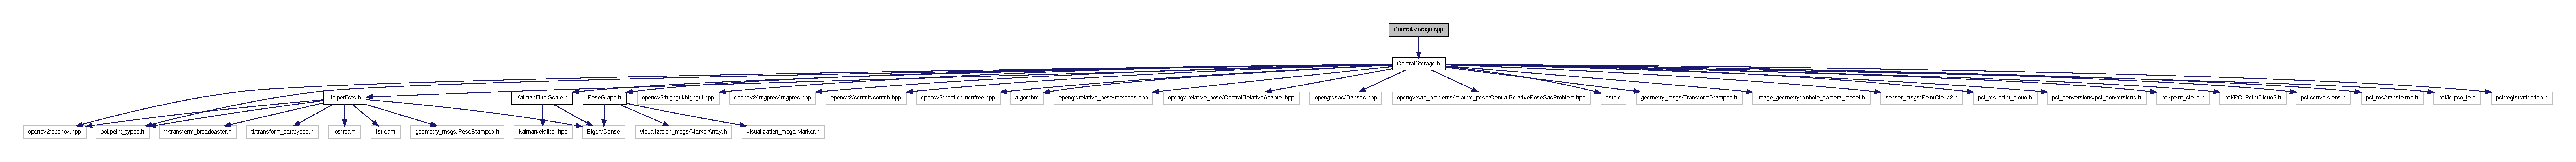
\includegraphics[width=350pt]{CentralStorage_8cpp__incl}
\end{center}
\end{figure}

\hypertarget{CentralStorage_8h}{\section{\-Central\-Storage.\-h \-File \-Reference}
\label{CentralStorage_8h}\index{\-Central\-Storage.\-h@{\-Central\-Storage.\-h}}
}
{\ttfamily \#include $<$opencv2/opencv.\-hpp$>$}\*
{\ttfamily \#include $<$opencv2/highgui/highgui.\-hpp$>$}\*
{\ttfamily \#include $<$opencv2/imgproc/imgproc.\-hpp$>$}\*
{\ttfamily \#include $<$opencv2/contrib/contrib.\-hpp$>$}\*
{\ttfamily \#include \char`\"{}opencv2/nonfree/nonfree.\-hpp\char`\"{}}\*
{\ttfamily \#include $<$algorithm$>$}\*
{\ttfamily \#include $<$opengv/relative\-\_\-pose/methods.\-hpp$>$}\*
{\ttfamily \#include $<$opengv/relative\-\_\-pose/\-Central\-Relative\-Adapter.\-hpp$>$}\*
{\ttfamily \#include $<$opengv/sac/\-Ransac.\-hpp$>$}\*
{\ttfamily \#include $<$opengv/sac\-\_\-problems/relative\-\_\-pose/\-Central\-Relative\-Pose\-Sac\-Problem.\-hpp$>$}\*
{\ttfamily \#include $<$cstdio$>$}\*
{\ttfamily \#include $<$geometry\-\_\-msgs/\-Transform\-Stamped.\-h$>$}\*
{\ttfamily \#include $<$image\-\_\-geometry/pinhole\-\_\-camera\-\_\-model.\-h$>$}\*
{\ttfamily \#include $<$sensor\-\_\-msgs/\-Point\-Cloud2.\-h$>$}\*
{\ttfamily \#include $<$pcl\-\_\-ros/point\-\_\-cloud.\-h$>$}\*
{\ttfamily \#include $<$pcl/point\-\_\-types.\-h$>$}\*
{\ttfamily \#include $<$pcl\-\_\-conversions/pcl\-\_\-conversions.\-h$>$}\*
{\ttfamily \#include $<$pcl/point\-\_\-cloud.\-h$>$}\*
{\ttfamily \#include $<$pcl/\-P\-C\-L\-Point\-Cloud2.\-h$>$}\*
{\ttfamily \#include $<$pcl/conversions.\-h$>$}\*
{\ttfamily \#include $<$pcl\-\_\-ros/transforms.\-h$>$}\*
{\ttfamily \#include $<$pcl/io/pcd\-\_\-io.\-h$>$}\*
{\ttfamily \#include $<$pcl/registration/icp.\-h$>$}\*
{\ttfamily \#include \char`\"{}\-Helper\-Fcts.\-h\char`\"{}}\*
{\ttfamily \#include \char`\"{}\-Kalman\-Filter\-Scale.\-h\char`\"{}}\*
{\ttfamily \#include \char`\"{}\-Pose\-Graph.\-h\char`\"{}}\*
\-Include dependency graph for \-Central\-Storage.\-h\-:\nopagebreak
\begin{figure}[H]
\begin{center}
\leavevmode
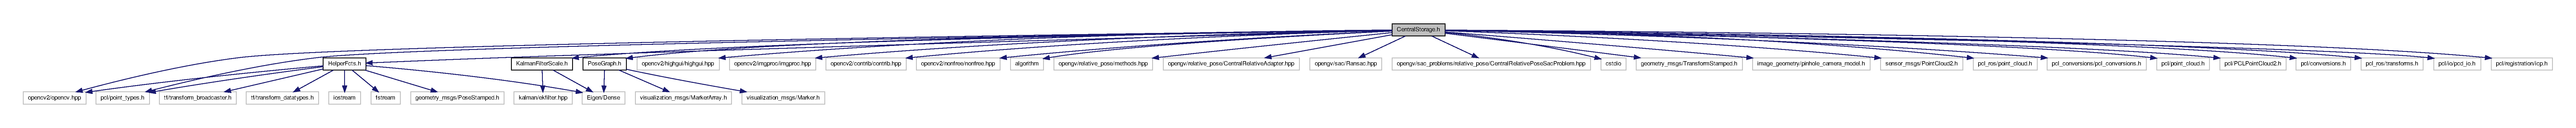
\includegraphics[width=350pt]{CentralStorage_8h__incl}
\end{center}
\end{figure}
\-This graph shows which files directly or indirectly include this file\-:\nopagebreak
\begin{figure}[H]
\begin{center}
\leavevmode
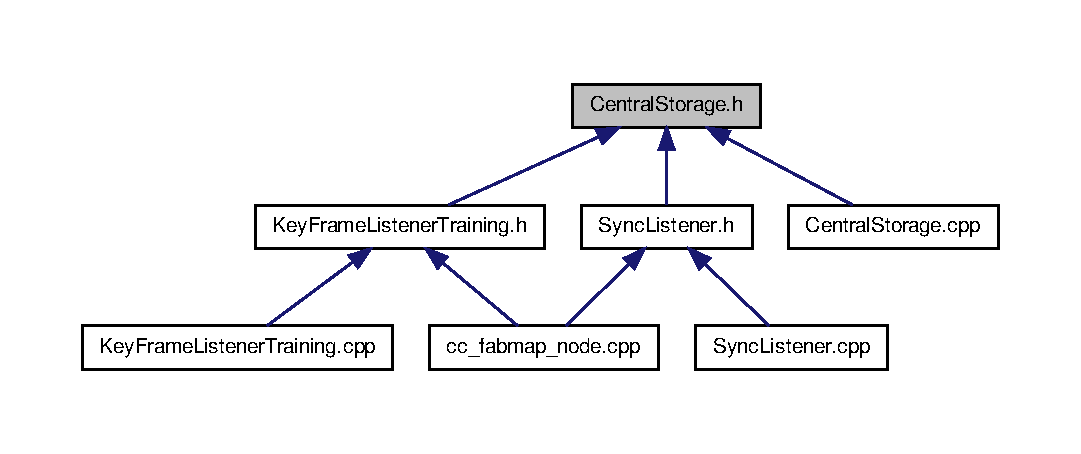
\includegraphics[width=350pt]{CentralStorage_8h__dep__incl}
\end{center}
\end{figure}
\subsection*{\-Classes}
\begin{DoxyCompactItemize}
\item 
struct \hyperlink{structkeyFrame}{key\-Frame}
\item 
class \hyperlink{classCentralStorage}{\-Central\-Storage}
\begin{DoxyCompactList}\small\item\em \-Class storing all images of all robots, global maps (pose graph and point cloud) \end{DoxyCompactList}\end{DoxyCompactItemize}

\hypertarget{HelperFcts_8cpp}{\section{\-Helper\-Fcts.\-cpp \-File \-Reference}
\label{HelperFcts_8cpp}\index{\-Helper\-Fcts.\-cpp@{\-Helper\-Fcts.\-cpp}}
}
{\ttfamily \#include \char`\"{}\-Helper\-Fcts.\-h\char`\"{}}\*
\-Include dependency graph for \-Helper\-Fcts.\-cpp\-:\nopagebreak
\begin{figure}[H]
\begin{center}
\leavevmode
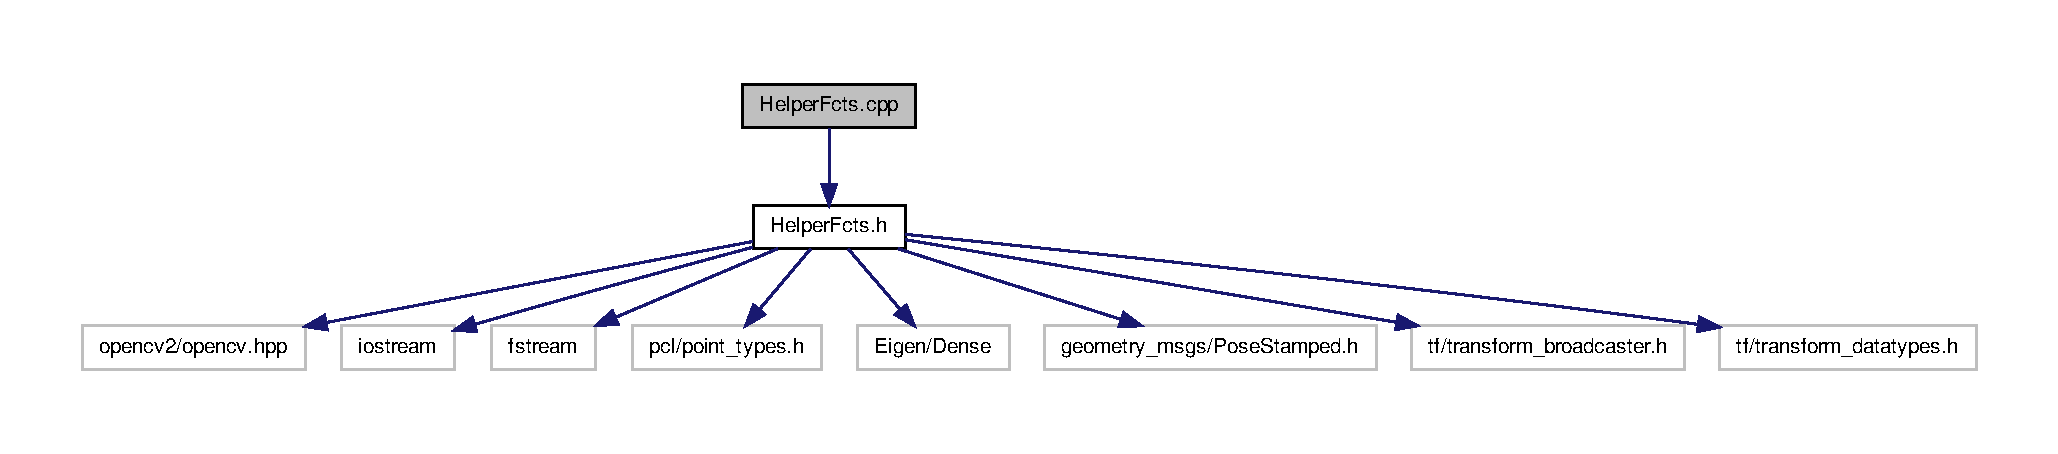
\includegraphics[width=350pt]{HelperFcts_8cpp__incl}
\end{center}
\end{figure}

\hypertarget{HelperFcts_8h}{\section{\-Helper\-Fcts.\-h \-File \-Reference}
\label{HelperFcts_8h}\index{\-Helper\-Fcts.\-h@{\-Helper\-Fcts.\-h}}
}
{\ttfamily \#include $<$opencv2/opencv.\-hpp$>$}\*
{\ttfamily \#include $<$iostream$>$}\*
{\ttfamily \#include $<$fstream$>$}\*
{\ttfamily \#include $<$pcl/point\-\_\-types.\-h$>$}\*
{\ttfamily \#include $<$\-Eigen/\-Dense$>$}\*
{\ttfamily \#include $<$geometry\-\_\-msgs/\-Pose\-Stamped.\-h$>$}\*
{\ttfamily \#include $<$tf/transform\-\_\-broadcaster.\-h$>$}\*
{\ttfamily \#include $<$tf/transform\-\_\-datatypes.\-h$>$}\*
\-Include dependency graph for \-Helper\-Fcts.\-h\-:\nopagebreak
\begin{figure}[H]
\begin{center}
\leavevmode
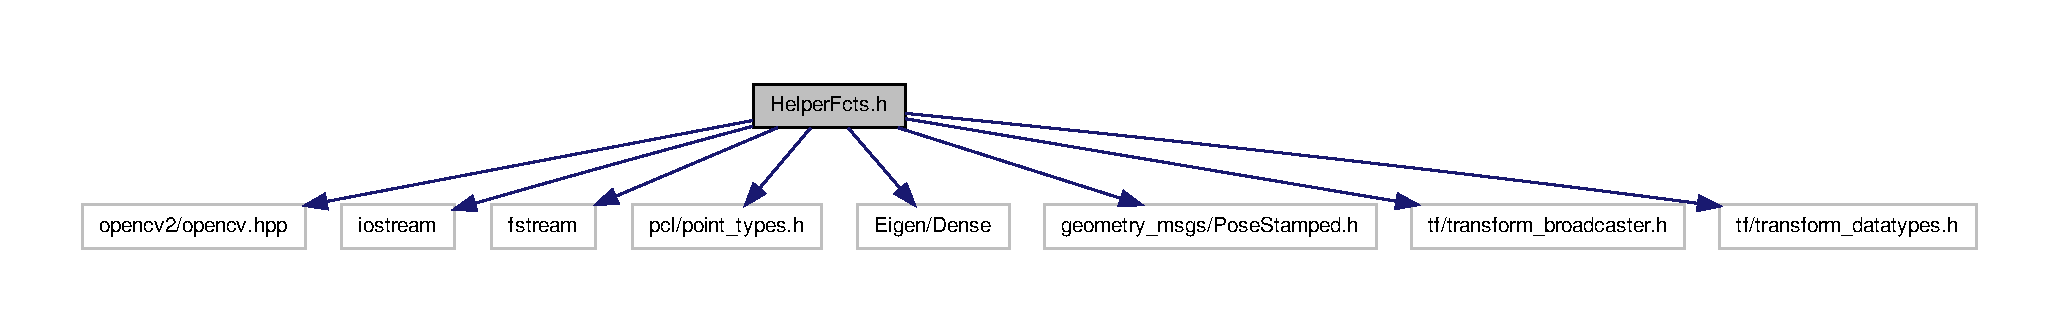
\includegraphics[width=350pt]{HelperFcts_8h__incl}
\end{center}
\end{figure}
\-This graph shows which files directly or indirectly include this file\-:\nopagebreak
\begin{figure}[H]
\begin{center}
\leavevmode
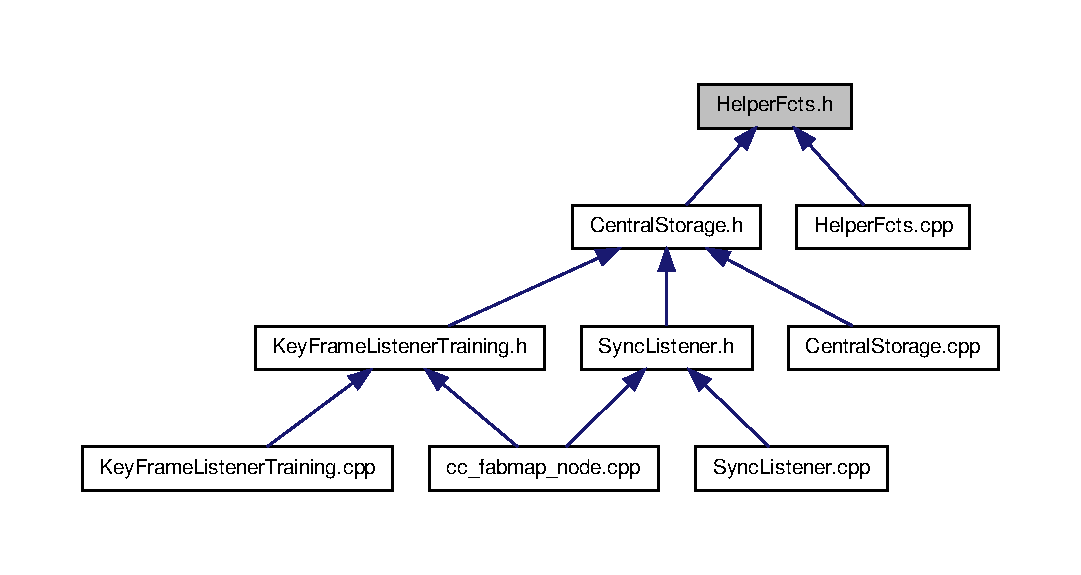
\includegraphics[width=350pt]{HelperFcts_8h__dep__incl}
\end{center}
\end{figure}
\subsection*{\-Classes}
\begin{DoxyCompactItemize}
\item 
class \hyperlink{classHelperFcts}{\-Helper\-Fcts}
\end{DoxyCompactItemize}

\hypertarget{KalmanFilterScale_8cpp}{\section{\-Kalman\-Filter\-Scale.\-cpp \-File \-Reference}
\label{KalmanFilterScale_8cpp}\index{\-Kalman\-Filter\-Scale.\-cpp@{\-Kalman\-Filter\-Scale.\-cpp}}
}
{\ttfamily \#include \char`\"{}\-Kalman\-Filter\-Scale.\-h\char`\"{}}\*
\-Include dependency graph for \-Kalman\-Filter\-Scale.\-cpp\-:\nopagebreak
\begin{figure}[H]
\begin{center}
\leavevmode
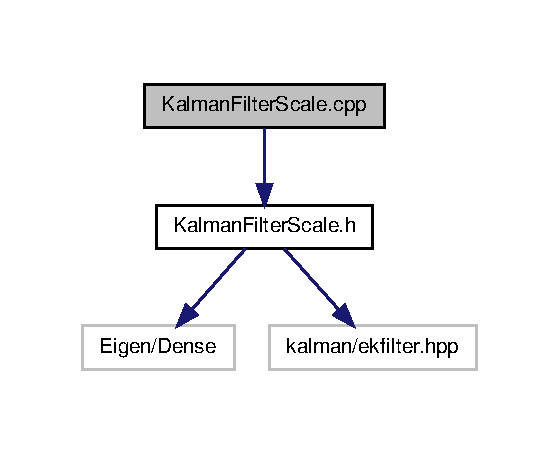
\includegraphics[width=268pt]{KalmanFilterScale_8cpp__incl}
\end{center}
\end{figure}

\hypertarget{KalmanFilterScale_8h}{\section{\-Kalman\-Filter\-Scale.\-h \-File \-Reference}
\label{KalmanFilterScale_8h}\index{\-Kalman\-Filter\-Scale.\-h@{\-Kalman\-Filter\-Scale.\-h}}
}
{\ttfamily \#include $<$\-Eigen/\-Dense$>$}\*
{\ttfamily \#include $<$kalman/ekfilter.\-hpp$>$}\*
\-Include dependency graph for \-Kalman\-Filter\-Scale.\-h\-:\nopagebreak
\begin{figure}[H]
\begin{center}
\leavevmode
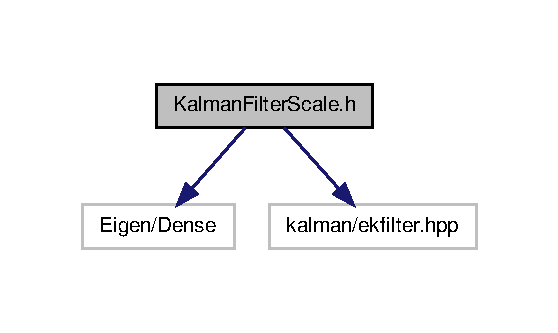
\includegraphics[width=268pt]{KalmanFilterScale_8h__incl}
\end{center}
\end{figure}
\-This graph shows which files directly or indirectly include this file\-:\nopagebreak
\begin{figure}[H]
\begin{center}
\leavevmode
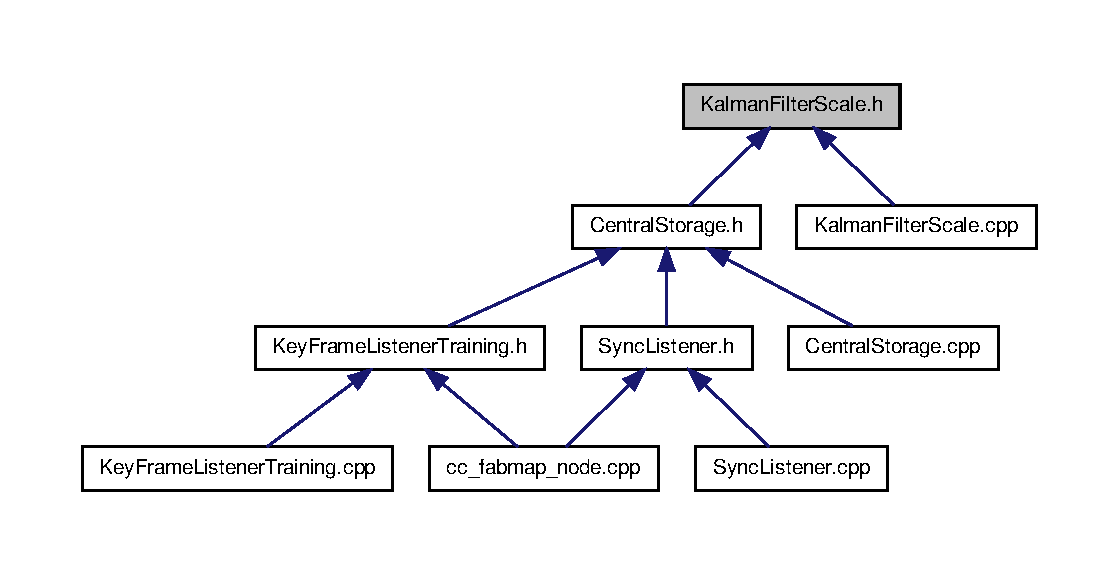
\includegraphics[width=350pt]{KalmanFilterScale_8h__dep__incl}
\end{center}
\end{figure}
\subsection*{\-Classes}
\begin{DoxyCompactItemize}
\item 
class \hyperlink{classKalmanFilterScale}{\-Kalman\-Filter\-Scale}
\end{DoxyCompactItemize}

\hypertarget{KeyFrameListenerTraining_8cpp}{\section{\-Key\-Frame\-Listener\-Training.\-cpp \-File \-Reference}
\label{KeyFrameListenerTraining_8cpp}\index{\-Key\-Frame\-Listener\-Training.\-cpp@{\-Key\-Frame\-Listener\-Training.\-cpp}}
}
{\ttfamily \#include \char`\"{}\-Key\-Frame\-Listener\-Training.\-h\char`\"{}}\*
\-Include dependency graph for \-Key\-Frame\-Listener\-Training.\-cpp\-:\nopagebreak
\begin{figure}[H]
\begin{center}
\leavevmode
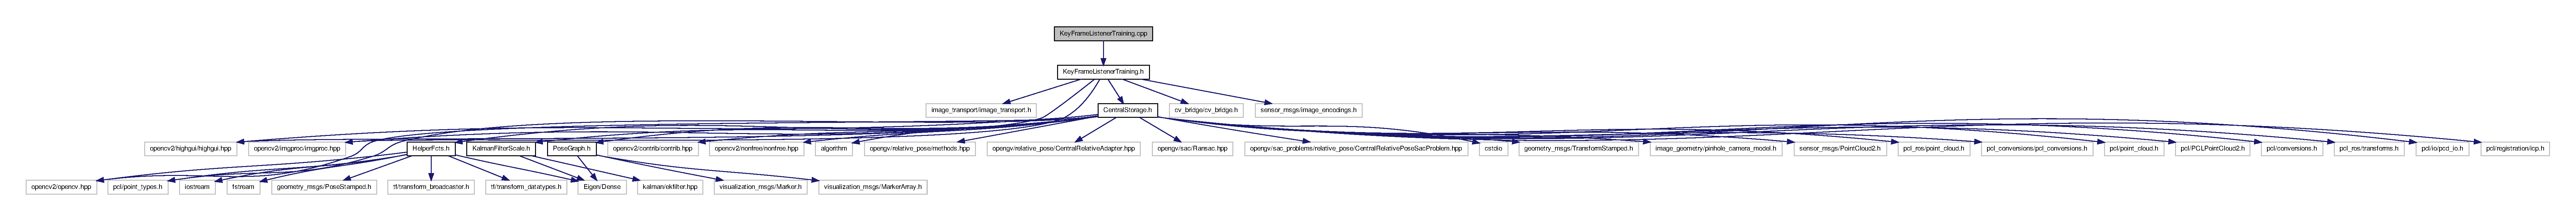
\includegraphics[width=350pt]{KeyFrameListenerTraining_8cpp__incl}
\end{center}
\end{figure}

\hypertarget{KeyFrameListenerTraining_8h}{\section{\-Key\-Frame\-Listener\-Training.\-h \-File \-Reference}
\label{KeyFrameListenerTraining_8h}\index{\-Key\-Frame\-Listener\-Training.\-h@{\-Key\-Frame\-Listener\-Training.\-h}}
}
{\ttfamily \#include $<$image\-\_\-transport/image\-\_\-transport.\-h$>$}\*
{\ttfamily \#include $<$opencv2/highgui/highgui.\-hpp$>$}\*
{\ttfamily \#include $<$cv\-\_\-bridge/cv\-\_\-bridge.\-h$>$}\*
{\ttfamily \#include $<$sensor\-\_\-msgs/image\-\_\-encodings.\-h$>$}\*
{\ttfamily \#include $<$opencv2/imgproc/imgproc.\-hpp$>$}\*
{\ttfamily \#include \char`\"{}\-Central\-Storage.\-h\char`\"{}}\*
\-Include dependency graph for \-Key\-Frame\-Listener\-Training.\-h\-:\nopagebreak
\begin{figure}[H]
\begin{center}
\leavevmode
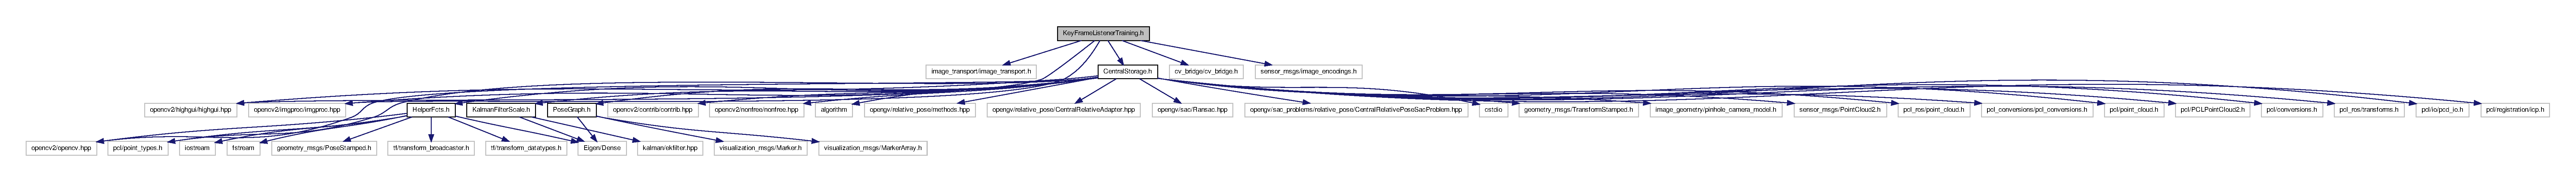
\includegraphics[width=350pt]{KeyFrameListenerTraining_8h__incl}
\end{center}
\end{figure}
\-This graph shows which files directly or indirectly include this file\-:\nopagebreak
\begin{figure}[H]
\begin{center}
\leavevmode
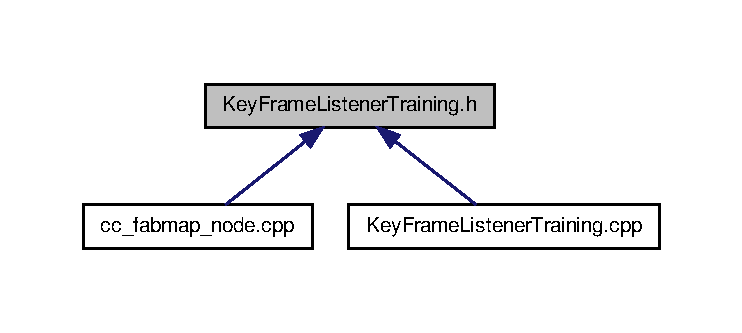
\includegraphics[width=350pt]{KeyFrameListenerTraining_8h__dep__incl}
\end{center}
\end{figure}
\subsection*{\-Classes}
\begin{DoxyCompactItemize}
\item 
class \hyperlink{classKeyFrameListenerTraining}{\-Key\-Frame\-Listener\-Training}
\begin{DoxyCompactList}\small\item\em \-Class listening to incoming images, each instance of the class listens to one robot -\/$>$ do training. \end{DoxyCompactList}\end{DoxyCompactItemize}

\hypertarget{PoseGraph_8cpp}{\section{\-Pose\-Graph.\-cpp \-File \-Reference}
\label{PoseGraph_8cpp}\index{\-Pose\-Graph.\-cpp@{\-Pose\-Graph.\-cpp}}
}
{\ttfamily \#include \char`\"{}\-Pose\-Graph.\-h\char`\"{}}\*
\-Include dependency graph for \-Pose\-Graph.\-cpp\-:\nopagebreak
\begin{figure}[H]
\begin{center}
\leavevmode
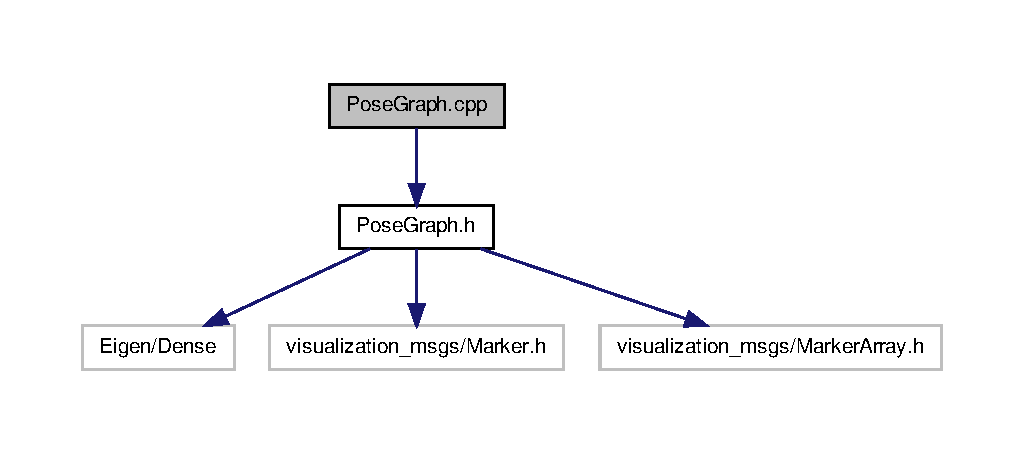
\includegraphics[width=350pt]{PoseGraph_8cpp__incl}
\end{center}
\end{figure}

\hypertarget{PoseGraph_8h}{\section{\-Pose\-Graph.\-h \-File \-Reference}
\label{PoseGraph_8h}\index{\-Pose\-Graph.\-h@{\-Pose\-Graph.\-h}}
}
{\ttfamily \#include $<$\-Eigen/\-Dense$>$}\*
{\ttfamily \#include $<$visualization\-\_\-msgs/\-Marker.\-h$>$}\*
{\ttfamily \#include $<$visualization\-\_\-msgs/\-Marker\-Array.\-h$>$}\*
\-Include dependency graph for \-Pose\-Graph.\-h\-:\nopagebreak
\begin{figure}[H]
\begin{center}
\leavevmode
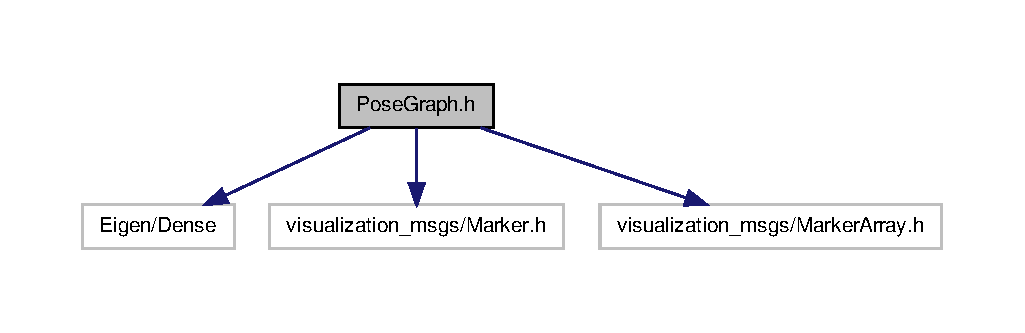
\includegraphics[width=350pt]{PoseGraph_8h__incl}
\end{center}
\end{figure}
\-This graph shows which files directly or indirectly include this file\-:\nopagebreak
\begin{figure}[H]
\begin{center}
\leavevmode
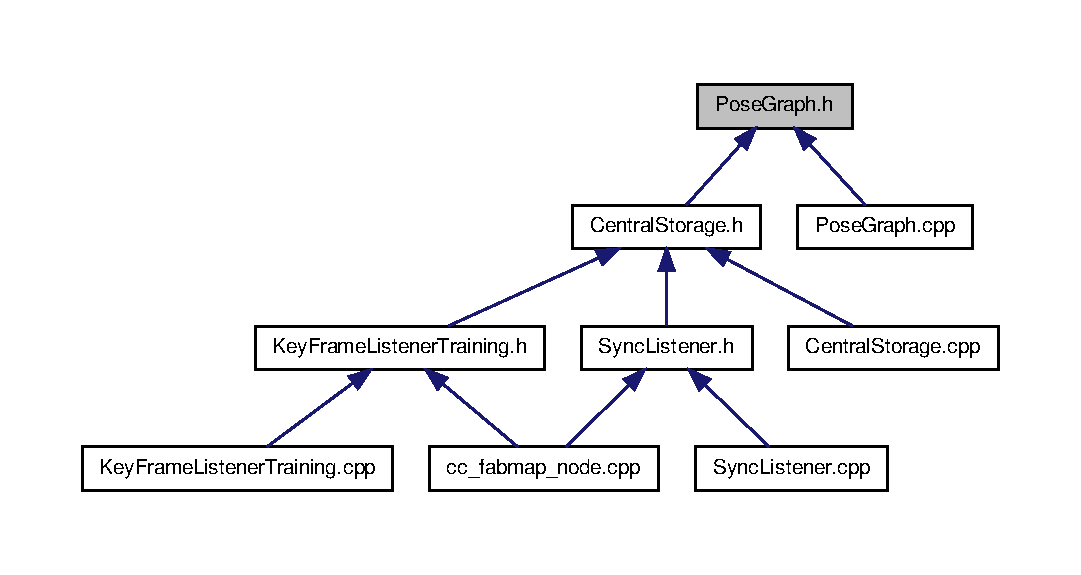
\includegraphics[width=350pt]{PoseGraph_8h__dep__incl}
\end{center}
\end{figure}
\subsection*{\-Classes}
\begin{DoxyCompactItemize}
\item 
class \hyperlink{classNode}{\-Node}
\item 
class \hyperlink{classEdge}{\-Edge}
\item 
class \hyperlink{classPoseGraph}{\-Pose\-Graph}
\end{DoxyCompactItemize}

\hypertarget{SyncListener_8cpp}{\section{\-Sync\-Listener.\-cpp \-File \-Reference}
\label{SyncListener_8cpp}\index{\-Sync\-Listener.\-cpp@{\-Sync\-Listener.\-cpp}}
}
{\ttfamily \#include \char`\"{}\-Sync\-Listener.\-h\char`\"{}}\*
\-Include dependency graph for \-Sync\-Listener.\-cpp\-:\nopagebreak
\begin{figure}[H]
\begin{center}
\leavevmode

\includegraphics[width=350pt]{SyncListener_8cpp__incl}
\end{center}
\end{figure}
\subsection*{\-Functions}
\begin{DoxyCompactItemize}
\item 
void \hyperlink{SyncListener_8cpp_a45d750f090ea9402b709498a49ecfa25}{lsd\-S\-L\-A\-M\-I\-D\-To\-F\-I\-D} (\hyperlink{classCentralStorage}{\-Central\-Storage} $\ast$storage, int lsd\-S\-L\-A\-M\-I\-D, int \&f\-I\-D)
\end{DoxyCompactItemize}


\subsection{\-Function \-Documentation}
\hypertarget{SyncListener_8cpp_a45d750f090ea9402b709498a49ecfa25}{\index{\-Sync\-Listener.\-cpp@{\-Sync\-Listener.\-cpp}!lsd\-S\-L\-A\-M\-I\-D\-To\-F\-I\-D@{lsd\-S\-L\-A\-M\-I\-D\-To\-F\-I\-D}}
\index{lsd\-S\-L\-A\-M\-I\-D\-To\-F\-I\-D@{lsd\-S\-L\-A\-M\-I\-D\-To\-F\-I\-D}!SyncListener.cpp@{\-Sync\-Listener.\-cpp}}
\subsubsection[{lsd\-S\-L\-A\-M\-I\-D\-To\-F\-I\-D}]{\setlength{\rightskip}{0pt plus 5cm}void {\bf lsd\-S\-L\-A\-M\-I\-D\-To\-F\-I\-D} (
\begin{DoxyParamCaption}
\item[{{\bf \-Central\-Storage} $\ast$}]{storage, }
\item[{int}]{lsd\-S\-L\-A\-M\-I\-D, }
\item[{int \&}]{f\-I\-D}
\end{DoxyParamCaption}
)}}\label{SyncListener_8cpp_a45d750f090ea9402b709498a49ecfa25}


\-Definition at line 9 of file \-Sync\-Listener.\-cpp.


\begin{DoxyCode}
                                                                       {
        bool found = false;
        typedef std::map<int,keyFrame> kFMap;
        for (kFMap::iterator it=storage->kFrames.begin(); it!=storage->kFrames.
      end(); ++it) {
                if(found == true) {
                        continue;
                }
                if(it->second.lsdSLAMID == lsdSLAMID) {
                        fID = it->second.fID;
                        found = true;
                }
        }
}
\end{DoxyCode}

\hypertarget{SyncListener_8h}{\section{\-Sync\-Listener.\-h \-File \-Reference}
\label{SyncListener_8h}\index{\-Sync\-Listener.\-h@{\-Sync\-Listener.\-h}}
}
{\ttfamily \#include $<$ros/ros.\-h$>$}\*
{\ttfamily \#include $<$message\-\_\-filters/subscriber.\-h$>$}\*
{\ttfamily \#include $<$message\-\_\-filters/synchronizer.\-h$>$}\*
{\ttfamily \#include $<$message\-\_\-filters/sync\-\_\-policies/approximate\-\_\-time.\-h$>$}\*
{\ttfamily \#include $<$std\-\_\-msgs/\-Float32.\-h$>$}\*
{\ttfamily \#include $<$sensor\-\_\-msgs/\-Image.\-h$>$}\*
{\ttfamily \#include $<$sensor\-\_\-msgs/\-Camera\-Info.\-h$>$}\*
{\ttfamily \#include $<$sensor\-\_\-msgs/\-Point\-Cloud2.\-h$>$}\*
{\ttfamily \#include $<$sensor\-\_\-msgs/image\-\_\-encodings.\-h$>$}\*
{\ttfamily \#include $<$geometry\-\_\-msgs/\-Pose\-Stamped.\-h$>$}\*
{\ttfamily \#include \char`\"{}cc\-\_\-fabmap/keyframe\-Msg\-Stamped.\-h\char`\"{}}\*
{\ttfamily \#include \char`\"{}cc\-\_\-fabmap/keyframe\-Graph\-Msg\-Stamped.\-h\char`\"{}}\*
{\ttfamily \#include \char`\"{}cc\-\_\-fabmap/keyframe\-Msg.\-h\char`\"{}}\*
{\ttfamily \#include \char`\"{}cc\-\_\-fabmap/keyframe\-Graph\-Msg.\-h\char`\"{}}\*
{\ttfamily \#include $<$cv\-\_\-bridge/cv\-\_\-bridge.\-h$>$}\*
{\ttfamily \#include $<$iostream$>$}\*
{\ttfamily \#include $<$pcl/io/pcd\-\_\-io.\-h$>$}\*
{\ttfamily \#include $<$pcl/point\-\_\-types.\-h$>$}\*
{\ttfamily \#include $<$pcl/filters/voxel\-\_\-grid.\-h$>$}\*
{\ttfamily \#include \char`\"{}\-Central\-Storage.\-h\char`\"{}}\*
\-Include dependency graph for \-Sync\-Listener.\-h\-:\nopagebreak
\begin{figure}[H]
\begin{center}
\leavevmode

\includegraphics[width=350pt]{SyncListener_8h__incl}
\end{center}
\end{figure}
\-This graph shows which files directly or indirectly include this file\-:\nopagebreak
\begin{figure}[H]
\begin{center}
\leavevmode
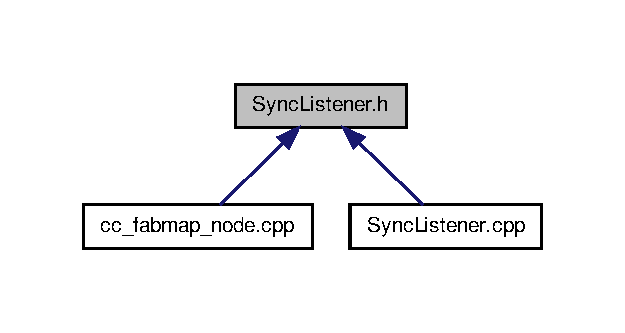
\includegraphics[width=300pt]{SyncListener_8h__dep__incl}
\end{center}
\end{figure}
\subsection*{\-Classes}
\begin{DoxyCompactItemize}
\item 
struct \hyperlink{structInputPointDense}{\-Input\-Point\-Dense}
\item 
struct \hyperlink{structGraphFramePose}{\-Graph\-Frame\-Pose}
\item 
struct \hyperlink{structGraphConstraint}{\-Graph\-Constraint}
\item 
class \hyperlink{classSyncListener}{\-Sync\-Listener}
\begin{DoxyCompactList}\small\item\em \-Class listening to incoming \-Msgs and synchronizes them, each instance of the class listens to one robot. \end{DoxyCompactList}\end{DoxyCompactItemize}

\printindex
\end{document}
